\documentclass{csnotes}

% ==============================================================================
% DOCUMENT SPECIFIC CUSTOMIZATIONS
% ==============================================================================

% --------------------------- START CUSTOMIZATIONS -----------------------------

% You can add any custom packages or commands specific to this document here
\newcommand{\SCal}{\mathcal{S}}
\NewDocumentCommand{\Prob}{o}{
  \IfNoValueTF{#1}
    {\mathbb{P}} % No condition
    {\mathbb{P}\left(#1\right)} % With condition
}
\NewDocumentCommand{\EV}{m o}{
  \IfNoValueTF{#2}
    {\mathbb{E}\left[#1\right]} % No condition
    {\mathbb{E}_{#2}\left[#1\right]} % With condition
}
\setabstracttitle{Scopo del documento}

\newcommand{\whitepage}{
  \newpage
  \thispagestyle{empty}
  \mbox{}
  \newpage
}

% ---------------------------- END CUSTOMIZATIONS ------------------------------



% ==============================================================================
% DOCUMENT INFORMATION
% ==============================================================================
\title{Encoding \& Encryption}
\author{Riccardo Elena, Fabrizio Apuzzo, Riccardo Regina}
\date{\today}

% Additional information for the title page
\university{Università degli Studi Federico II di Napoli}
\department{Dipartimento d'Ingegneria Elettrica e Tecnologie dell'Informazione}
\course{Corso di Laurea Magistrale in Computer Science}
\subject{Encoding \& Encryption}
\academicyear{Anno Accademico 2024/2025}

% ==============================================================================
% BIBLIOGRAPHY
% ==============================================================================
% Specify the .bib file with your bibliographic references
% Uncomment the following line when you have created the bibliography.bib file
% \addbibresource{bibliography.bib}

% ==============================================================================
% INIZIO DOCUMENTO
% ==============================================================================

\begin{document}

\pagenumbering{gobble}

\maketitlepage{}
\whitepage{}

\begin{abstract}
  Questo file contiene appunti e materiali di studio relativi al corso di Encoding \& Encryption tenuto dal Prof.~A.~De Luca alla Università degli Studi Federico II di Napoli nell'A.A.~25/26.
  
  Questo corso tratterà i fondamenti della codifica di sorgente e canale nell'ottica della teoria dell'informazione di Shannon, nonché i principi e le tecniche di crittografia moderna.

  \textbf{Questi appunti sono destinati a supportare gli studenti nel loro percorso di apprendimento e a fornire una risorsa di riferimento per gli argomenti discussi durante il corso, ma non sostituiscono in alcun modo il materiale ufficiale e le lezioni del docente.}
  Questo documento è prodotto da studenti, per studenti, e potrebbe dunque contenere errori o imprecisioni. Feedback e correzioni sono ben accetti e incentivati, e possono essere inviati tramite pull request o issue nella \href{https://github.com/RiccardoElena/E-E_Notes}{repository GitHub del documento}.

  A tal proposito, nel documento saranno presenti alcuni contenuti non provenienti direttamente dalle lezioni, ma aggiunti o modificati dagli autori per migliorare la comprensibilità o l'approfondimento degli argomenti trattati.
  Ci impegniamo a verificare col docente ogni modifica sostanziale al materiale originale, ma in caso tale verifica non fosse ancora avvenuta, verranno inseriti degli indicatori per segnalare le eventuali divergenze dal materiale ufficiale.
  In particolare:
  \begin{itemize}
    \item I contenuti aggiunti o modificati in maniera sostanziale dagli autori saranno segnalati con il simbolo \warningsymbol{}
    \item I contenuti che invece hanno subito esclusivamente riorganizzazione strutturale o di formattazione verranno segnalati col simbolo \infosymbol{}
    \item Eventuali contenuti aggiuntivi, non presentati a lezione ma verificati col docente, saranno segnalati con il simbolo \extrasymbol{}
  \end{itemize}
  
  % Firma autori / link repo (posizionata come firma in basso a destra)
  \begin{flushright}
    \vspace{2cm}
    \textbf{Gli Autori:}\\
    \href{https://github.com/RiccardoElena}{Riccardo Elena}, \href{https://github.com/TheFabbest}{Fabrizio Apuzzo}, \href{https://github.com/riccardoregina}{Riccardo Regina} \\
  \end{flushright}
\end{abstract}
\whitepage{}

\newgeometry{top=2cm}
\tableofcontents
\restoregeometry{}

\whitepage{}

\pagenumbering{arabic}
\setcounter{page}{1}

\chapter{Prerequisiti di Algebra}

Prima di iniziare a trattare gli argomenti principali del corso,
è necessario ripassare alcuni concetti di algebra alla base della teoria dei codici introducendone alcuni nuovi.

In particolare questo capitolo si concentra sulle strutture algebriche di semigruppi e monoidi e di loro proprietà utili per la teoria dei codici.

Inizialmente però, per addentrarci nelle definizioni delle suddette strutture algebriche, è necessario introdurre alcune notazioni preliminari, che verranno conservate per tutto il corso di questi appunti.

\section{Nozioni Preliminari}

Le lettere maiuscole \(A, B, X, Y \ldots\) indicheranno generalmente insiemi, che siano finiti o infiniti.
Per quanto riguarda gli insiemi numerici tradizionali, useremo:
\begin{itemize}
  \item \(\N = \set{0,1,2,\ldots}\) per i numeri naturali (incluso lo zero);
  \item \(\N_+ = \set{1,2,3,\ldots}\) per i numeri naturali positivi (escluso lo zero);
  \item \(\Z\) per i numeri interi;
  \item \(\Q\) per i numeri razionali;
  \item \(\R\) per i numeri reali.
\end{itemize}
Con eventuali notazioni aggiuntive a pedice per indicare sottoinsiemi particolari (ad esempio \(\R_{\geq 0}\) per i numeri reali non negativi).

Per ogni insieme \(X\), \(\mathcal{P}(X)\) denota l'insieme delle parti di \(X\), ovvero l'insieme di tutti i sottoinsiemi di \(X\) e \(\#X\) la sua cardinalità.
Gli elementi di tali insiemi saranno indicati con le lettere minuscole corrispondenti \(a,b,x,y \ldots\), in particolare con la lettera \(n\) a indicare un generico elemento naturale se non specificato diversamente.

\section{Semigruppi e Monoidi}
\begin{definition}{Semigruppo}
  Un \keyword{semigruppo} è una coppia \((S, \cdot)\) dove \(S\) è un insieme non vuoto e \(\cdot : S \times S \to S\) è un'operazione binaria associativa, ovvero:
  \[\forall a,b,c \in S, (a \cdot b) \cdot c = a \cdot (b \cdot c).\]
\end{definition}

Questa struttura algebrica è molto generica, imponendo solo l'associatività dell'operazione binaria.
Un esempio di semigruppo è dato da \((\N',+)\) dove l'operazione binaria è la somma tra numeri naturali positivi ordinaria.

\begin{definition}{Monoide}
  Un \keyword{monoide} \((M,\cdot,1_M)\) è un semigruppo \((M, \cdot)\) dotato di elemento neutro \(1_M\) per l'operazione binaria\footnote{Denotato semplicemente \(1\) in caso di non ambiguità del monoide di riferimento}, ovvero:
  \[\forall a \in M, a \cdot 1_M = 1_M \cdot a = a\]
\end{definition}

\begin{example}{}
  \begin{itemize}
    \item \((\N, +)\) è un monoide con elemento neutro \(0\).
    \item \((\N, \cdot)\) è un monoide con elemento neutro \(1\).
    \item Dato \(T\) insieme, sia \((\mathcal{P}(T), \cup, \emptyset)\) che \((\mathcal{P}(T), \cap, T)\) sono monoidi.
  \end{itemize}
  Gli esempi precedenti sono tutti monoidi commutativi (o abeliani), ovvero tali che:
  \[\forall a,b \in M, a \cdot b = b \cdot a.\]
  Un esempio di monoide non abeliano è, dato un insieme \(T\), il monoide delle funzioni totali da \(T\) in sé stesso \((T^{T}, \circ, id_T)\) dove l'operazione binaria è la composizione di funzioni e l'elemento neutro è la funzione identità su \(T\).
\end{example}

\subsection{Proprietà di monoidi e semigruppi}

Analizziamo ora alcune notazioni e proprietà di monoidi e semigruppi.

\begin{definition}[label=obs:power_notation]{}
  Dato \((M,\cdot,1_M)\) monoide, si ha che, \(\forall m \in M\), \(m^0 = 1_M\) e \(m^{n+1} = m \cdot m^n, \quad \forall n \geq 0\).
\end{definition}

\begin{definition}{Morfismi di semigruppi e monoidi}
  Siano \((S,\cdot)\) e \((T,*)\) semigruppi.
  Una funzione \(f: S \to T\) è un \keyword{morfismo di semigruppi} se:
  \[\forall a,b \in S, f(a \cdot b) = f(a) * f(b).\]
  Se \(S\) e \(T\) sono monoidi, \(f\) è un \keyword{morfismo di monoidi} se è un morfismo di semigruppi e:
  \[f(1_S) = 1_T.\]
  Se \(f\) è iniettiva, si dice che è un \keyword{monomorfismo}, se è suriettiva si dice che è un \keyword{epimorfismo}, se è biunivoca si dice che è un \keyword{isomorfismo}.
  In quest'ultimo caso, i due semigruppi (o monoidi) si dicono isomorfi.
\end{definition}

\begin{example}{}
  Consideriamo i monoidi \((\N, +, 0)\) e \((\N, \cdot, 1)\).
  La funzione 
  \[f: \N \to \N\]
  \[f:n \mapsto f(n) = 2^n\]
  è un monomorfismo tra i due monoidi.
  Infatti,
  \[f(n+m) = 2^{n+m} = 2^n \cdot 2^m = f(n) \cdot f(m)\]
  \[ f(0) = 2^0 = 1\]
  Tuttavia, \(f\) non è un epimorfismo, poiché non è suriettiva (ad esempio, non esiste \(n \in \N\) tale che \(f(n) = 3\)).
\end{example}

\begin{definition}{Sottosemigruppo e Sottomonoide}
  Sia \((S,\cdot_S)\) un semigruppo.
  \(T \subseteq S\) è un \keyword{sottosemigruppo} di \(S\) (\(T \leq S\)), se \(T\) è chiusa rispetto all'operazione binaria di \(S\), ovvero:
  \[\forall a,b \in T, a \cdot_S b \in T\]
  Dato \((M,\cdot_M,1_M)\) è un monoide, \(N \subseteq M\) è un \keyword{sottomonoide} di \(M\) (\(N \leq M\)) se:
  \begin{itemize}
    \item \(N\) è un sottosemigruppo di \(M\);
    \item \(1_M \in N\).
  \end{itemize}
\end{definition}

Dato un qualsiasi semigruppo \((S,\cdot)\), è possibile costruire un semigruppo sul suo insieme delle parti \(\mathcal{P}(S)\) indotto dall'operazione binaria di \(S\).
\begin{definition}{Semigruppo delle parti}
  Sia \((S,\cdot)\) un semigruppo.
  Definiamo l'operazione binaria \(\circ\) su \(\mathcal{P}(S)\) come:
  \[\forall X,Y \in \mathcal{P}(S), X \circ Y = \set{x \cdot y}[ x \in X, y \in Y].\]
\end{definition}
Tale costruzione è estendibile anche a un qualsiasi monoide \((M,\cdot,1_M)\), usando come elemento neutro l'insieme \(\set{1_M}\).

Questo semigruppo (o monoide) delle parti è particolarmente rilevante, poiché, grazie alle notazioni introdotte nella \Cref{obs:power_notation}, è possibile definire le potenze di un qualsiasi sottoinsieme \(Y \subseteq S\).

Tale notazione permette di formulare in modo più compatto la chiusura di un sottoinsieme \(Y\) di un semigruppo.
  \[(\forall a,b \in T, a \cdot_S b \in T)\iff (Y^2 \subseteq Y).\]

\begin{definition}{Sottostruttura generata}
  Sia \((S,\cdot)\) un semigruppo e \(Y \subseteq S\).
  Definiamo il \keyword{sottosemigruppo} di \(S\) generato da \(Y\) come:
  \[Y^+ = Y \cup Y^2 \cup Y^3 \cup \cdots = \bigcup_{n=1}^{\infty} Y^n\]
  l'insieme di tutte le possibili combinazioni finite di elementi di \(Y\) tramite l'operazione binaria di \(S\).

  Dato \((M,\cdot_M,1_M)\) monoide, è possibile aggiungere la potenza zero, definendo il \keyword{sottomonoide} di \(M\) generato da \(Y\) come:
  \[Y^* = \set{1_S} \cup Y^+ = \bigcup_{n=0}^{\infty} Y^n.\]
\end{definition}

\begin{definition}{Base di un semigruppo (monoide)}
  Sia \(S\) un semigruppo (monoide).
  Una \keyword{base} di \(S\) è un sottoinsieme \(X \subseteq S\) che gode di \emph{univoca fattorizzazione}, ovvero che dati \(\forall x_1,x_2,\ldots,x_n,x_1',x_2',\ldots,x_m' \in X\) si ha che:
  \[x_1 x_2 \ldots x_n = x_1' x_2' \ldots x_m' \implies n=m \land x_1 = x_1' \land x_2 = x_2' \land \ldots \land x_n = x_n'\]
\end{definition}
In altre parole, ogni elemento di \(X^{+}\) si fattorizza in un unico modo come prodotto di elementi di \(X\).

\begin{observation}[label=obs:no_neutral_in_base]{}
  Per definizione di base, nessuna base di un monoide può contenere l'elemento neutro.
  Infatti, se \(1_M \in X\), \(\forall x \in X\) si ha che \(1_M \cdot x = x\), quindi ogni elemento di \(X^{+}\) si fattorizza in un modo non univoco.
\end{observation}

\begin{definition}{Semigruppi e monoidi liberi}
  Data \(X \subseteq S\) base di un semigruppo \(S\), si dice che \(S\) è \keyword{libero} se \(S = X^{+}\).
  Analogamente, dato \(X \subseteq M\) base di un monoide \(M\), si dice che \(M\) è \keyword{libero} se \(M = X^{*}\).
\end{definition}
Un modo meno formale ma più intuitivo di definire un semigruppo (monoide) libero è quella di considerarlo il semigruppo (monoide) con la minor quantità di vincoli possibile, ovvero solo quelli imposti dalla definizione di semigruppo (monoide).
La struttura è \emph{libera} poiché non ha vincoli aggiuntivi che la limitano, essendo dunque la più generale possibile dato l'insieme sottostante.
Tale proprietà di generalità verrà formalizzata più avanti tramite una proprietà universale.
\begin{proposition}{Unicità della base in un semigruppo (monoide) libero}
  Sia \(S\) un semigruppo libero, allora l'unica base di \(S\) è \(S \setminus S^2\), ovvero l'insieme degli elementi di \(S\) che non sono esprimibili come prodotto di altri elementi di \(S\).
  Analogamente, sia \(M\) un monoide libero, allora l'unica base di \(M\) è \((M\setminus \{1_M\}) \setminus {(M\setminus \{1_M\})}^2\).
\end{proposition}

\begin{theorem}{Proprietà universale dei monoidi (semigruppi) liberi}
  Sia \(M\) un monoide con \(X \subseteq M\). Allora \(M\) è libero di base \(X\) se e solo se, per ogni monoide \(M'\) e ogni applicazione \(f: X \to M'\), esiste un unico morfismo di monoidi \(\bar{f}: M \to M'\) tale che \(\hat{f}_{|_X} = f\), ovvero tale che il seguente diagramma commuta:
  \begin{center}
      \begin{tikzcd}[column sep=huge, row sep=huge, cells={nodes={scale=1.2, transform shape}}]
        X \arrow[r, "f"] \arrow[d, hook,"i"] & M' \\ %chktex 18 
        M \arrow[ru, dashed, "\exists!\bar{f}"'] & %chktex 18
      \end{tikzcd}
  \end{center}
  Vale a dire che \(\bar{f} \circ i = f\), dove \(i: X \hookrightarrow M\) è l'inclusione di \(X\) in \(M\).\footnote{È possibile vedere \(i\) anche come la riduzione dell'identità di \(M\) a \(X\), ovvero \(i = id_{M|_X}\).}
  Tale formulazione ha carattere algebrico-universale e quindi può essere estesa anche ai semigruppi, oltre che a qualsiasi famiglia di algebre dello stesso tipo, quali per esempio i gruppi.
\end{theorem}

In altre parole, esiste un unico morfismo \(\bar{f}\) da \(M\) a \(M'\) che estende \(f\) morfismo da \(X\) a \(M'\); se così non è, allora \(M\) non è libero di base \(X\).
È importante notare che la proprietà universale, dato un monoide \(M\) e una sua base \(X\) vale \emph{per ogni monoide \(M'\)}, e quindi in particolare anche per \(M' = M\).
Da questa particolare circostanza è facile ricavare che \(id_M: M \to M\) è l'unico morfismo da \(M\) a \(M\) che estende \(id_X\).

\begin{corollary}{}
  Sia \(M\) monoide libero di base \(X\) e \(M'\) monoide libero di base \(X'\).
  Se \(\#X = \#X'\), allora \(M\) e \(M'\) sono isomorfi.
\end{corollary}

\begin{proof}
  Per dimostrare tale corollario sarà sufficiente mostrare che è possibile costruire un morfismo biettivo (isomorfismo) tra \(M\) e \(M'\)
  Essendo le basi equipotenti, esiste una biiezione \(g: X \leftrightarrow X'\).
  Consideriamo l'applicazione \(f = i' \circ g : X \to M'\), dove \(i': X' \hookrightarrow M'\), ovvero l'inclusione di \(X'\) in \(M'\).
  Per la proprietà universale, esiste un unico morfismo di monoidi \(\bar{f}: M \to M'\) tale che \(\bar{f}_{|_X} = f\).
  Analogamente, sia \(f'= i \circ g^{-1} : X' \to M\) e sia \(\bar{f'}: M' \to M\) l'unico morfismo di monoidi tale che \(\bar{f'}_{|_{X'}} = f'\).
  Si ha che \(\bar{f'} \circ \bar{f}: M \to M\) è un morfismo di monoidi che estende \(id_X\), ovvero:
  \[\forall x \in X, \bar{f'} (\bar{f}(x)) = \bar{f'}(g(x))= g^{-1}(g(x))= x\]
  Come detto precedentemente però \(id_M\) è l'unico morfismo di monoidi da \(M\) in sé stesso che estende \(id_X\), dunque necessariamente si ha che \(\bar{f'} \circ \bar{f} = id_M\)
  Dalla definizione di biettività abbiamo che \(\bar{f} = \bar{f'}^{-1} \), ovvero che \(\bar{f}\) è un isomorfismo tra \(M\) e \(M'\). 
\end{proof}
Questo corollario mostra che, a meno di isomorfismi, il monoide libero \(A^*\) è l'unico monoide libero con base di cardinalità \(\#A\).

Dato un monoide libero \(M\) è possibile definire un morfismo di lunghezza delle parole.
\begin{definition}{Morfismo di lunghezza}
  Sia \(M\) un monoide libero di base \(X\).
  Il \keyword{morfismo di lunghezza} è \(|\;|: M \to(\N,+,0)\) tale che \[\forall x \in X, |x| = 1\]
\end{definition}

\begin{observation}{}
  È importate notare che il morfismo di lunghezza è ben definito per ogni valore di \(M\), poiché ogni elemento di \(M\) si fattorizza in modo univoco come prodotto di elementi di \(X\).
  Non fosse stato così, non sarebbe possibile definire in modo univoco la lunghezza di un elemento di \(M\) a partire dagli elementi della sua base.
\end{observation}

\begin{lemma}[label=lem:levi]{Levi}
  Sia \(M\) un monoide libero, \(m_1,m_2,m_3,m_4 \in M\) tali che \(m_1m_2=m_3m_4 \text{ e } |m_1| \geq |m_3|\).
  Allora \(\exists v \in M: m_1 = m_3v \land vm_2 = m_4\)
\end{lemma}

\begin{proof}
  Chiamiamo \(w\) la parola comune \(m_1m_2 = m_3m_4\).
  Possiamo rappresentare la sua fattorizzazione in \(m_1m_2\) come:
  \begin{figure}[H]
    \centering
    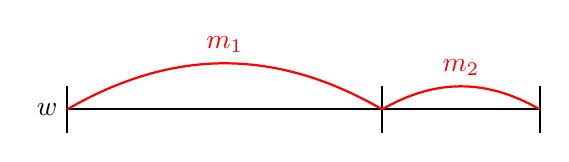
\begin{tikzpicture}
      \coordinate (A) at (0,0);
      \coordinate (B) at (6,0);
      \draw[thick] (A) -- (B);
      \foreach \x in {0,4,6}{
        \coordinate (P\x) at (\x,0);
        \draw[thick] (P\x) -- ++(0,-0.3);
        \draw[thick] (P\x) -- ++(0,0.3);
      }
      \node[left] at (A) {\(w\)};
      \draw[thick, red, bend left] (A) to node[midway, above, red] {\(m_1\)} (P4);
      \draw[thick, red,bend left] (P4) to node[midway, above, red] {\(m_2\)} (P6);
    \end{tikzpicture}
  \end{figure}
  e la fattorizzazione in \(m_3m_4\) come:
  \begin{figure}[H]
    \centering
    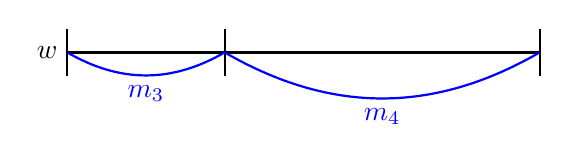
\begin{tikzpicture}
      \coordinate (A) at (0,0);
      \coordinate (B) at (6,0);
      \draw[thick] (A) -- (B);
      \foreach \x in {0,2,6}{
        \coordinate (P\x) at (\x,0);
        \draw[thick] (P\x) -- ++(0,-0.3);
        \draw[thick] (P\x) -- ++(0,0.3);
      }
      \node[left] at (A) {\(w\)};
      \draw[thick, blue,bend right] (A) to node[midway, below, blue] {\(m_3\)} (P2);
      \draw[thick, blue,bend right] (P2) to node[midway, below, blue] {\(m_4\)} (P6);
    \end{tikzpicture}
  \end{figure}
  Se \(\abs{m_1} = \abs{m_3}\), dall'ipotesi che \(M\) è libero segue che \(m_1 = m_3\) e \(m_2 = m_4\).
  Questo perché, non fossero uguali, si avrebbe una doppia fattorizzazione di \(w\), in contraddizione con la definizione di base.
  Il teorema in questo caso è verificato ponendo \(v = \varepsilon\).

  Nel caso \(\abs{m_1} > \abs{m_3}\) invece, il punto di divisione tra \(m_1\) e \(m_2\) si trova a destra del punto di divisione tra \(m_3\) e \(m_4\).
  Di conseguenza, è possibile sovrapporre le rappresentazioni precedenti come segue:
  \begin{figure}[H]
    \centering
    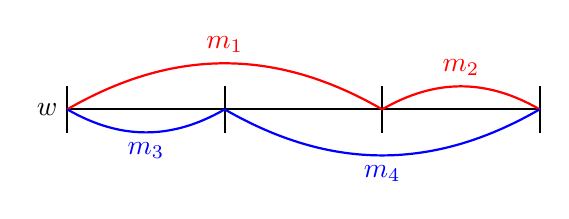
\begin{tikzpicture}
      \coordinate (A) at (0,0);
      \coordinate (B) at (6,0);
      \draw[thick] (A) -- (B);
      \foreach \x in {0,2,4,6}{
        \coordinate (P\x) at (\x,0);
        \draw[thick] (P\x) -- ++(0,-0.3);
        \draw[thick] (P\x) -- ++(0,0.3);
      }
      \node[left] at (A) {\(w\)};
      \draw[thick, red, bend left] (A) to node[midway, above, red] {\(m_1\)} (P4);
      \draw[thick, red,bend left] (P4) to node[midway, above, red] {\(m_2\)} (P6);
      \draw[thick, blue,bend right] (A) to node[midway, below, blue] {\(m_3\)} (P2);
      \draw[thick, blue,bend right] (P2) to node[midway, below, blue] {\(m_4\)} (P6);
    \end{tikzpicture}
  \end{figure}
  Chiamando \(v\) la parola compresa tra i due punti di divisione si ha che \(m_1 = m_3v\) e \(vm_2 = m_4\).
  Anche in questo caso, se una delle due uguaglianze non fosse verificata, si avrebbe una doppia fattorizzazione di \(w\), in contraddizione con la definizione di base.
  \begin{figure}
    \centering
    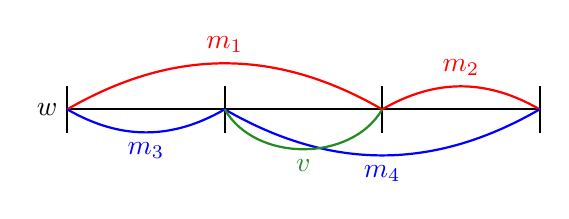
\begin{tikzpicture}
      \coordinate (A) at (0,0);
      \coordinate (B) at (6,0);
      \draw[thick] (A) -- (B);
      \foreach \x in {0,2,4,6}{
        \coordinate (P\x) at (\x,0);
        \draw[thick] (P\x) -- ++(0,-0.3);
        \draw[thick] (P\x) -- ++(0,0.3);
      }
      \node[left] at (A) {\(w\)};
      \draw[thick, red, bend left] (A) to node[midway, above, red] {\(m_1\)} (P4);
      \draw[thick, red,bend left] (P4) to node[midway, above, red] {\(m_2\)} (P6);
      \draw[thick, blue,bend right] (A) to node[midway, below, blue] {\(m_3\)} (P2);
      \draw[thick, blue,bend right] (P2) to node[midway, below, blue] {\(m_4\)} (P6);
      \draw[thick, ForestGreen, bend right=60] (P2) to node[midway, below, ForestGreen] {\(v\)} (P4);
    \end{tikzpicture}
  \end{figure}
\end{proof}

\begin{definition}[label=def:quotient_sets]{Insiemi quoziente}
  Siano \(Y,Z \subseteq M\) monoide. Definiamo gli insiemi quoziente destro e sinistro come:
  \begin{equation}
    \begin{aligned}
      Y^{-1}Z &= \set{m \in M}[ \exists y \in Y, ym \in Z]\\
      ZY^{-1} &= \set{m \in M}[ \exists y \in Y, my \in Z]
    \end{aligned}
  \end{equation}
\end{definition}

In altre parole, possiamo vedere $Y^{-1}Z$ come l'insieme di quegli $m\in M$ che, messi a destra di un $y\in Y$, stanno in $Z$.

\begin{theorem}[label=thm:schützenberger_monoids]{Schützenberger sui sottomonoidi liberi}
  Sia \(M\) libero e \(N \leq M\). Allora \(N \text{ è libero } \iff N^{-1}N \cap NN^{-1} \subseteq N\)
\end{theorem}
In altre parole questo teorema ci dice che \(N\) sottomonoide di \(M\) libero è a sua volta libero se e solo se ogni parola di \(M\) che completa sia a destra che a sinistra parole di \(N\) sia a sua volta inclusa in \(N\).
Tale formulazione può essere espressa formalmente come:
\[N \text{ libero } \iff \left(\forall m \in M (\exists n_1,n_2,n_3,n_4( n_1m=n_2 \land mn_3=n_4) \implies m \in N)\right)\]

\begin{observation}{}
  Se \(N\leq M\) necessariamente \(N \subseteq N^{-1}N \cap NN^{-1}\) poiché tutte le parole di \(N\) completano sia a destra che a sinistra la parola vuota per formare se stesse.
  Di conseguenza il teorema può essere riformulato equivalentemente come:
  \begin{theorem}{Schützenberger alt.}
    Sia \(M\) libero e \(N \leq M\). Allora \(N \text{ è libero } \iff N^{-1}N \cap NN^{-1} = N\)
  \end{theorem}
  In altre parole un sottomonoide di un monoide libero è esso stesso libero se non contiene più del necessario.
\end{observation}

\begin{proof}[\extrasymbol{} Dimostrazione di~\ref{thm:schützenberger_monoids}]
  In caso uno qualsiasi tra \(n_1,n_2,n_3,n_4 \in N\) e \(m \in M\) sia l'elemento neutro \(1_M\) la doppia implicazione è verificata in maniera banale.
  Assumendo dunque che tutti gli elementi coinvolti siano diversi da \(1_M\) andiamo a dimostrare i due versi della doppia implicazione:
  \begin{description}
    \item[\q{\(\implies\)}]
      Supponiamo che \(N\) sia libero, e siano \(m \in M, n_1,n_2,n_3,n_4 \in N\) tali che\footnote{Possiamo assumere che esistano, poiché altrimenti il predicato che vogliamo verificare sarebbe banalmente vero per implicazione vacua} \(n_1m = n_2\) e \(mn_3 = n_4\).
      Si ha dunque che
      \[n_1 m n_3 = n_2 n_3 \implies n_1 n_4 = n_2 n_3\]
      Sia dunque \(X\) base di \(N\). Siano \(a_1, \ldots, a_h, b_1, \ldots, b_k, c_1, \ldots, c_i, d_1, \ldots, d_j \in X\) tali che
      \[n_1 = a_1 \ldots a_h, n_2 = b_1 \ldots b_k, n_3 = c_1 \ldots c_i, n_4 = d_1 \ldots d_j\]
      Dall'uguaglianza precedente segue che
      \[a_1 \ldots a_h d_1 \ldots d_j = b_1 \ldots b_k c_1 \ldots c_i\]
      Essendo \(N\) libero, tale fattorizzazione è unica, dunque necessariamente \(h+j = k+i\) e che \(a_1 = b_1\).
      
      Possiamo dunque rappresentare tale parola come segue:
      \begin{figure}[H]
        \centering
        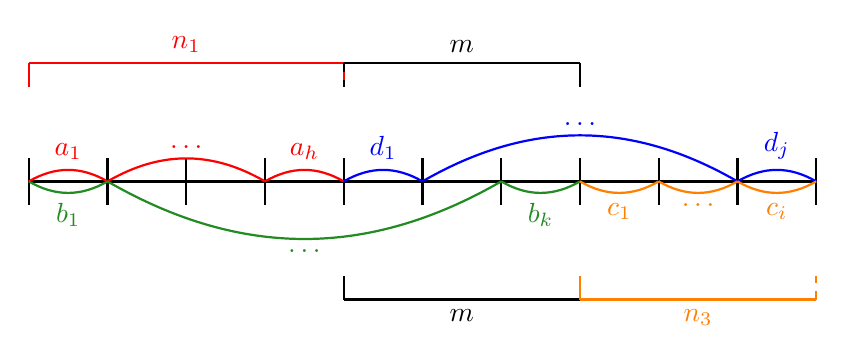
\begin{tikzpicture}
          \foreach \x in {0,1,2,3,4,5,6,7,8,9,10}{
            \coordinate (P\x) at (\x,0);
            \draw[thick] (P\x) -- ++(0,-0.3);
            \draw[thick] (P\x) -- ++(0,0.3);
            }
          \draw[thick] (P0) -- (P10);
            % \node[left] at (A) {\(n_1 m n_3 = n_2 n_3\)};
          \draw[thick, red, bend left] (P0) to node[midway, above, red] {\(a_1\)} (P1);
          \draw[thick, red, bend left] (P1) to node[midway, above, red] {\(\ldots\)} (P3);
          \draw[thick, red,bend left] (P3) to node[midway, above, red] {\(a_h\)} (P4);
          \draw[thick, blue,bend left] (P4) to node[midway, above, blue] {\(d_1\)} (P5);
          \draw[thick, blue,bend left] (P5) to node[midway, above, blue] {\(\ldots\)} (P9);
          \draw[thick, blue,bend left] (P9) to node[midway, above, blue] {\(d_j\)} (P10);

          \draw[thick, ForestGreen, bend right] (P0) to node[midway, below, ForestGreen] {\(b_1\)} (P1);
          \draw[thick, ForestGreen, bend right] (P1) to node[midway, below, ForestGreen] {\(\ldots\)} (P6);
          \draw[thick, ForestGreen,bend right] (P6) to node[midway, below, ForestGreen] {\(b_k\)} (P7);
          \draw[thick, orange,bend right] (P7) to node[midway, below, orange] {\(c_1\)} (P8);
          \draw[thick, orange,bend right] (P8) to node[midway, below, orange] {\(\ldots\)} (P9);
          \draw[thick, orange,bend right] (P9) to node[midway, below, orange] {\(c_i\)} (P10);

          \draw[thick, red] (0,1.5) to node[midway, above, red] {\(n_1\)} (4,1.5);
          \draw[thick,red] (0,1.5) -- ++(0,-0.3);
          \draw[thick, red] (4,1.5) -- ++(0,-0.3);
          \draw[thick] (4,1.5) to node[midway, above] {\(m\)} (7,1.5);
          \draw[thick,dashed] (4,1.5) -- ++(0,-0.3);
          \draw[thick] (7,1.5) -- ++(0,-0.3);

          \draw[thick] (4,-1.5) to node[midway, below] {\(m\)} (7,-1.5);
          \draw[thick] (4,-1.5) -- ++(0,+0.3);
          \draw[thick] (7,-1.5) -- ++(0,+0.3);
          \draw[thick, orange] (7,-1.5) to node[midway, below, orange] {\(n_3\)} (10,-1.5);
          \draw[thick, orange,dashed] (10,-1.5) -- ++(0,+0.3);
          \draw[thick, orange] (7,-1.5) -- ++(0,+0.3);
          
        \end{tikzpicture}
      \end{figure}
    
      Si ha dunque che \(m = b_{h+1}\ldots b_k = d_1 \ldots d_{j-i}\), e dunque \(m \in N\).
    \item[\q{\(\impliedby\)}]
      Supponiamo che \(N^{-1}N \cap NN^{-1} \subseteq N\).
      Sia inoltre \(X = (N\setminus \set{1})\setminus{(N\setminus \set{1})}^2\) e supponiamo per assurdo che \(X\) non sia una base di \(N\).
      Esistono dunque \(x_1, \ldots, x_i, x_1', \ldots, x_j' \in X\) tali che \(x_1\ldots x_i = x_1'\ldots x_j'\) con \(x_1 \neq x_1'\).
      Senza perdita di generalità, supponiamo che \(\abs{x_1} < \abs{x_1'}\).
      Per il lemma di Levi (\ref{lem:levi}) esiste \(v \in M\) tale che \(x_1' = x_1 v\) e \(x_2 \ldots x_i = v x_2' \ldots x_j'\).
      Ponendo \(m = v, n_1 = x_1, n_2 = x_1', n_3 = x_2'\ldots x_j', n_4 =  x_2 \ldots x_i\), dall'ipotesi segue che \(v \in N\).
      Ma \(x_1 \in X \implies x_1 \in N\), e dunque \(x_1' = x_1 v \in {(N\setminus\set{1})}^2\), in contraddizione con la definizione di \(X\).
      Dunuque \(X\) è una base di \(N\), e \(N\) è libero.
  \end{description}
\end{proof}

% Esempio di sottomonoide non libero è ad esempio qualsiasi monoide generato da un qualsiasi \(X \subseteq \N\setminus {1}\) ristpetto all'addizione.

\begin{definition}{Sottomoide unitario}
  Dato \(M\) monoide, \(N \leq M\) è detto \keyword{unitario a sinistra} (rispettivamente a destra) se:
  \[N^{-1}N \subseteq N \text{ sx}\]
  \[NN^{-1} \subseteq N \text{ dx}\]
  \(N\) si dice \keyword{unitario} se è unitario a sinistra o a destra.
\end{definition}

% se è unitario è libero non viceversa
Da tale definizione e dal teorema~\ref{thm:schützenberger_monoids} segue che, dato \(M\) monoide libero, se  \(N \leq M\) è unitario, allora è libero.


Finita la parte introduttiva su gli strumenti matematici necessari,
possiamo finalmente addentrarci nel primo capitolo: i codici.
\chapter{Codici}
In questo capitolo, affronteremo le nozioni di base della Teoria dei Codici.

\section{Monoide delle parole, linguaggi, codici}
\begin{definition}{Monoide delle parole}
  Definiamo $(A, \cdot, \varepsilon)$ il monoide delle parole con alfabeto $A$. Dunque, $A^{+}$ è l'insieme di tutte le parole non vuote, mentre $A^{*}\cup \{\varepsilon\}$ è l'insieme di tutte le parole, inclusa quella vuota.
\end{definition}

\begin{definition}{Linguaggio}
  Dato \(A\) alfabeto finito, diremo che \(\emptyset \neq X \subseteq A^*\) è un \keyword{linguaggio}.
\end{definition}

\begin{definition}{Codice}
  Dato \(A\) alfabeto finito, diremo che \(\emptyset \neq X \subseteq A^*\) è un \keyword{codice} se \(X\) è base.
\end{definition}

\begin{observation}{}
  Come già osservato nella \Cref{obs:no_neutral_in_base}, per definizione di base, nessun codice può contenere la parola vuota \(\varepsilon\).
  Di conseguenza, la notazione \(X \subseteq A^*\) può essere sostituita con \(X \subseteq A^+\) se \(X\) è codice.
\end{observation}

\begin{definition}[label=def:prefix_suffix]{Prefisso e Suffisso}
  Dato \(A\) alfabeto finito, diremo che \(\emptyset \neq X \subseteq A^*\) è
  \begin{description}
    \item[\keyword{Prefisso}] se \(X\cap XA^+ = \emptyset\)
    \item[\keyword{Suffisso}] se \(A^+X \cap X = \emptyset\)
  \end{description}
\end{definition}

In altre parole \(X\) è prefisso se nessuna parola di \(X\) è prefisso di un'altra parola di \(X\), e analogamente per il suffisso.

Il concetto di codice e di prefisso (suffisso) sono strettamente collegati.
È possibile infatti dimostrare due forti risultati a riguardo.
\begin{theorem}[label=thm:prefix_suffix_code]{}
  Sia \(A\) alfabeto finito e \(\emptyset \neq X \subseteq A^*\).
  Allora:
  \begin{enumerate}
    \item \(X\) prefisso (suffisso) è codice \(\iff X \neq \set{\varepsilon}\)
    \item \(X\) codice è prefisso (suffisso) \(\iff X^*\) unitario a sinistra (destra)
  \end{enumerate}
\end{theorem}

\section{Insiemi Resto e Decisione dei Codici}
Vedremo adesso dei criteri per determinare se un linguaggio $X$ è codice o meno. Un primo criterio derivante dal capitolo precedente è illustrato di seguito.

\begin{corollary}{}
  \(\emptyset \neq X \subseteq A^+\) è codice se e solo se valgono entrambe le seguenti condizioni:
  \begin{itemize}
    \item \({(X^*)}^{-1}X^* \cap X^*{(X^*)}^{-1} \subseteq X^* \), ovvero $X^{*}$ rispetta \ref{thm:schützenberger_monoids} e quindi è libero;
    \item \(X \cap XX^+ = \emptyset\), ovvero $X$ è la base di $X^{*}$.
  \end{itemize}
\end{corollary}
Tuttavia, verificare che $X^{*}$ sia libero mediante \ref{thm:schützenberger_monoids} risulta molto complicato. Pertanto, introdurremo dei metodi di più facile applicazione. Prima però, dobbiamo introdurre dei concetti.

Dagli insiemi quozienti, definiti nella \Cref{def:quotient_sets}, è possibile definire gli insiemi \emph{resto} da essi derivati.
\begin{definition}[label=def:remainder]{Insiemi resto}
  Per \(X \subseteq A^+\) definiamo la successione di insiemi resto destri come:
  \begin{equation}
    R_n=\begin{cases}
      X^{-1}X\setminus \set{\varepsilon} & n = 1\\
      X^{-1} R_{n-1}(X) \cup {R_{n-1}(X)}^{-1}X, & n > 1\\
    \end{cases}
  \end{equation}
  I resti sinistri possono essere definiti in modo analogo usando il quoziente destro.
\end{definition}

In altre parole, dato \(X \subseteq A^+\), il primo insieme dei resti destri \(R_1(X)\) si ottiene come segue: si confrontano tra loro tutte le parole di $X$: se una parola $x_1 \in X$ è prefisso di un'altra parola $x_{2} \in X$, ovvero si ha $x_2=x_1 v$, con $v \in A^{*}$, allora si inserisce $v$ in $R_1(X)$.
Insiemi di resto successivi si ottengono con lo stesso procedimento ma confrontando prima parole di $X$ con parole del resto precedente e poi parole del resto precedente con parole di $X$.

Tali insiemi sono collegati a importanti proprietà dei codici, come vedremo a breve.
\begin{note}{}
  Se \(X\) è chiaro dal contesto, indicheremo semplicemente con \(R_n\) i suoi insiemi resto.
\end{note}

\begin{example}{}
  Sia \(A = \set{a,b}, X = \set{a,a^3b,abb,b^3}\). Avremo dunque che gli insiemi resto di \(X\) sono: 
  \begin{itemize}
    \item \(R_1 = \set{a^2b, bb}\) con \(a^2b\) che completa \(a\) per formare \(a^3b\) e \(bb\) che completa sempre \(a\) per formare \(abb\).
    \item \(R_2 = \set{ab,b}\) con \(ab\) che completa sempre \(a\) per formare \(a^2b\) e \(b\) che completa \(bb\) per formare \(b^3\).
    \item \(R_3 = \set{b,bb}\) con \(b\) che completa \(a\) per formare \(ab\) e \(bb\) che completa \(b\) per formare \(bbb\). Da questo punto la successione si stabilizza, e dunque \(\forall n \geq 3, R_n = \set{b,bb}\)
  \end{itemize}
\end{example}

È interessante notare che l'\(X\) scelto nell'esempio precedente è un codice, e che i suoi insiemi resto non contengono mai elementi di \(X\).
Questa osservazione non è casuale, ma è in realtà il risultato del teorema di Sardinas-Patterson, che ci dà un metodo iterativo di facile applicazione per determinare se un linguaggio $X$ è codice.
\begin{theorem}[label=thm:sardinas-patterson]{Sardinas-Patterson}
  Sia \(\emptyset \neq X \subseteq A^+\). Allora \(X\) è codice \(\iff \forall n\geq 1\st R_n(X) \cap X = \emptyset\)
\end{theorem}

Per dimostrare questo teorema, è utile utilizzare un risultato intermedio per semplificare la trattazione.

\begin{lemma}[label=lem:sardinas-patterson-intermediate]{}
  Sia \(X \subseteq A^+\) e \(n\geq 1\). Allora, data \(w \in A^+\), \(w \in R_n \iff \exists i,j\geq 1, x_1,\ldots,x_i,x_1',\ldots,x_j' \in X\) tali che:
  \begin{itemize}
    \item \(i+j=n+1\)
    \item \(x_1\ldots x_{i}w = x_1'\ldots x_j'\), ovvero $w$ è la parte che manca alla sequenza $x_{i}, \dots, x_{j}$ per essere uguale a $x_{i}^{'}, \dots, x_{j}^{'}$;
    \item \(x_1 \neq x_1'\), per minimalità: se le due sequenze fossero uguali all'inizio, allora potremmo tagliarle e partire dai primi $x$,$x^{'}$ ad essere diversi. Questa condizione ci permette di prendere le due sequenze in modo minimale. Inoltre, se aggiungessimo una stessa sequenza a sinistra di ogni membro di (2), invalideremmo (1).
    \item \(\abs{w} \leq \abs{x_j'}\), ovvero $w$ è contenuta nell'ultima parola $x_{j}^{'}$ della sequenza $x_{1}^{'}, \dots, x_{j}^{'}$. Se ciò non fosse vero, $w$ si potrebbe scrivere come $w=x_{i+1}w^{'}$, eludendo la condizione (1).
  \end{itemize}
\end{lemma}

\begin{observation}{}
  Il lemma afferma che una parola $w$ appartiene al resto ennesimo $R_{n}$ se e solo se è possibile trovare $i$ parole di $X$ a cui, aggiungendo $w$, si ottengono $j$ parole di $X$, con $i+j=n+1$.

  Riprendiamo l'esempio precedente:
  \begin{itemize}
    \item $ab \in R_{2}$ poiché trovo $i=2$, $j=1$ (e quindi $i+j=3=2+1=n+1$) tali per cui $x_{1}x_{2}w=(a)(a)(ab)=a^{3}b=x^{'}_{1}$ con $|ab|\leq|ab|$;
    \item $b \in R_{2}$ poiché trovo $i=1$, $j=2$ tali per cui $x_{1}w=(ab^{2})(b)=(a)(b^{3})=x^{'}_{1}x^{'}_{2}$ con $|b|\leq|b^{3}|$.
  \end{itemize}
\end{observation}

\begin{proof}
  La dimostrazione procede per induzione su \(n\). Il passo base è banale: sia $n = 1$: $w \in R_{1} \iff \exists x,x^{'} \in X: xw=x^{'}$. Trovo $i=j=1$ per cui valgono tutte e quattro le condizioni.
  \begin{description}
    \item[\q{\(\implies\)}] 
      Avendo un resto, dobbiamo trovare $i$ e $j$ che soddisfano le quattro proprietà.

      \textbf{Passo induttivo}, $n > 1$:  $R_n = X^{-1}R_{n-1} \cup R_{n-1}^{-1}X$, quindi esistono $w \in X$ e $r_{n-1} \in R_{n-1}$ t.c. $xw=r_{n-1}$ (caso 1) oppure $r_{n-1}w=x$ (caso 2). Per $r_{n-1}$ vale la tesi: $\exists i, j \geq 1: x_{1}, \dots, x_{i}, x^{'}_{1}, \dots, x^{'}_{j} \in X$ con $i+j=n$ (1) e $x_{1}, \dots,x_{i}r_{n-1} = x^{'}_{1}, \dots, x^{'}_{j}$ (2) con $x_{1} \neq x^{'}_{1}$ (3) e $|r_{n-1}| \leq |x^{'}_{j}|$ (4).
      
      (Caso 1, $xw=r_{n-1}$) Sostituisco $r_{n-1}$ con $xw$ in $x_{1}, \dots,x_{i}r_{n-1} = x^{'}_{1}, \dots, x^{'}_{j}$ e ottengo $x_{1}, \dots,x_{i}xw = x^{'}_{1}, \dots, x^{'}_{j}$ per cui $i+1$ e $j$ verificano le quattro proprietà. 
      
      (Caso 2, $r_{n-1}w=x$) Moltiplico $w$ ad ambo i membri di $x_{1}, \dots,x_{i}r_{n-1} = x^{'}_{1}, \dots, x^{'}_{j}$, ottenendo $x_{1}, \dots,x_{i}r_{n-1}w = x^{'}_{1}, \dots, x^{'}_{j}w$ ma $r_{n-1}w = x$ per cui si ottiene $x_{1}, \dots,x_{i}x = x^{'}_{1}, \dots, x^{'}_{j}w$, ovvero ci siamo ritrovati nel caso 1 con l'unica differenza, non importante logicamente, che $w$ si trova all'altro membro. Quindi le quattro proprietà sono soddisfatte per $i+1$ e $j$.

    \item[\q{\(\impliedby\)}] 
      Abbiamo le due sequenze di parole con $i$ e $j$ t.c. valgono le quattro proprietà e dobbiamo far vedere che $w$ appartiene a $R_{n}$.
      \textbf{Passo induttivo}, $n > 1$: supponiamo che esistano 
      $i$ e $j$ t.c. le quattro proprietà siano soddisfatte.
      
      (Caso 1, $|x_{i}w| \leq |x_{j}^{'}|$) Si ha $i > 1$, poiché: 
      \begin{itemize}
        \item se $i=j=1$, allora $n=1$. $\bot$.
        \item se $i=1, j>1$, allora si ha $x_{1}w=x_{1}^{'}\dots x_{j}^{'}$. Affinché sia ancora vera l'ipotesi $x_{1}w=x^{'}_{1}\dots x^{'}_{j}$, poiché ciascuno degli $x_{1}^{'},\dots x_{j}^{'}$ ha lunghezza almeno $1$, deve verificarsi $|x_{1}w|>|x_{j}^{'}|$. $\bot$.  
      \end{itemize}
      
      Sia $r_{n-1}=x_{i}w$. Abbiamo, per ipotesi, $x_{1}\dots x_{i-1}x_{i}w=x_{1}^{'}\dots x_{j}^{'}$, ovvero, sostituendo $x_{i}w$ con $r_{n-1}$, $x_{1}\dots x_{i-1}r_{n-1}=x_{1}^{'}\dots x_{j}^{'}$ con $i-1+j=n$ e, per ipotesi, si ha $x_{1}\neq x_{1}^{'}$, $|r_{n-1}|<|x_{j}^{'}|$. Quindi, $i-1$ e $j$ soddisfano la tesi e allora $r_{n-1} \in R_{n-1}$. Poiché $r_{n-1}=x_{i}w$, ovvero $w$ è il completamento di $x_{i}$ affinché $x_{i}w=r_{n-1}$, e $r_{n-1} \in R_{n-1}$, allora $w \in R_{n}$.
    
      (Caso 2, $|x_{i}w| > |x_{j}^{'}|$) Si ha $j>1$, poiché: per la condizione 4, si ha $|w|<|x_{j}^{'}|$. Abbiamo quindi, $|w|<|x_{j}^{'}| \wedge |x_{i}w|>|x_{j}^{'}|$, da cui si capisce che $w$ è suffisso di $x_{j}^{'}$ e che quindi esiste un $v \in A^{*}$ t.c. $x_{j}^{'}=vw$. 

      Per ipotesi si ha $x_{1}\dots x_{i}w=x_{1}^{'}\dots x_{j}^{'}$ da cui, sostituendo $x_{j}^{'}=vw$, si ottiene $x_{1}\dots x_{i}\bcancel{w}=x_{1}^{'}\dots x_{j-1}^{'}v\bcancel{w}$. A questo punto, se $j=1$, si ha $x_{1}\dots x_{i}=v$ e, poiché ciascuno degli $x_{1},\dots x_{i-1}$ ha lunghezza almeno $1$, si ha $|x_{i}|<|v|$, che implica $|x_{i}w|<|vw|=|x_{j}^{'}|$. $\bot$

      Consideriamo nuovamente $x_{1}\dots x_{i}=x_{1}^{'}\dots x_{j-1}^{'}v$. Per $i$ e $j-1$ vale la tesi, quindi $v \in R_{n-1}$. Poichè $vw=x_{j}^{'}$, ovvero $w$ è il completamento di $v$ affinchè $vw=x_{j}^{'}$, e $v \in R_{n-1}$, allora $w \in R_{n}$.
  \end{description}
\end{proof}

Conclusa la dimostrazione del lemma, possiamo procedere con la dimostrazione del Teorema di Sardinas-Patterson.
\begin{proof}[Dimostrazione (\ref{thm:sardinas-patterson})]
  Vogliamo dimostrare l'asserto negato, ovvero: $X$ non è codice $\iff \exists n \geq 1:  R_{n} \cap X \neq \emptyset$.
  \begin{description}
    \item[\q{\(\implies\)}] 
      Se $X$ non è codice, allora non rispetta la proprietà di univoca fattorizzazione, quindi esistono due sequenze $x_{1},\dots x_{h},x_{1}^{'},\dots x_{k}^{'} \in X$ t.c. $x_{1}\dots x_{h}=x_{1}^{'}\dots x_{k}^{'}$, con $x_{1}\neq x_{1}^{'}$ per minimalità e quindi $h>1 \vee k>1$ necessariamente. Allora, si verifica la tesi del lemma scegliendo $i=h-1$ e $j=k$ t.c. $n=h-1+k-1$. Poichè uno tra $h$ e $k$ è maggiore di $1$, si ha $n\geq1$. Quindi il lemma garantisce $x_{k} \in R_{n}$.
    \item[\q{\(\impliedby\)}] 
      Se $\exists n:R_{n} \cap X \neq \emptyset$, allora esiste un $x \in R_{n}\cap X$ ed in particolare $x \in X$. Allora, per $x$ vale il lemma con $w=x$, ovvero il lemma garantisce l'esistenza di due sue fattorizzazioni. Quindi $X$ vìola la proprietà di univoca fattorizzazione, quindi non è codice.
  \end{description}
\end{proof}

\begin{observation}{}
  \begin{itemize}
    \item \(X \text{codice prefisso} \iff R_1 = \emptyset\).
      Questo poiché dalla definizione di prefisso si ha che \(X \cap XA^+ = \emptyset \iff X^{-1}X \setminus \set{\varepsilon} = \emptyset\)
    \item \(X \text{codice} \iff \forall n \geq 1, L_n \cap X = \emptyset\),
      dove \(L_n\) sono gli insiemi resto sinistri di \(X\).
      La dimostrazione è analoga a quella del \Cref{thm:sardinas-patterson}, utilizzando il corrispondente lemma per gli insiemi resto sinistri.
  \end{itemize}
\end{observation}

\begin{example}{}
  Sia \(X_2 = \set{a,ab,bb}\). Calcoliamo gli insiemi resto di \(X_2\):

  \(R_1 = X_2^{-1}X_2 \setminus \set{\varepsilon} = \set{b}\) poiché \(b\) completa \(a\) per formare \(ab\).

  \(R_2 = X_2^{-1}R_1 \cup R_1^{-1}X_2 = \set{b}\) poiché \(b\) completa \(a\) per formare \(ab\) e \(b\) completa \(bb\) per formare \(bb\).

  Da questo punto in poi, la successione si stabilizza, dunque \(\forall n \geq 1, R_n = \set{b}\). Poiché \(b \not\in X_2\), per il \Cref{thm:sardinas-patterson}, \(X_2\) è codice.

  Sia \(X_4 = \set{a,aba,bb}\). Calcoliamo gli insiemi resto di \(X_4\):
  
  \(R_1 = X_4^{-1}X_4 \setminus \set{\varepsilon} = \set{ba}\) poiché \(ba\) completa \(a\) per formare \(aba\).

  \(R_2 = X_4^{-1}R_1 \cup R_1^{-1}X_4 = \emptyset\) poiché nessuna parola di \(X_4\) può essere usata per completare \(ba\) e viceversa.
  
  Da questo punto in poi, la successione si stabilizza, dunque \(\forall n \geq 2, R_n = \emptyset\). Anche in questo caso, \(X_4\) è codice per il \Cref{thm:sardinas-patterson}.

  Sia infine \(X' = \set{a,ab,ba}\). Calcoliamo gli insiemi resto di \(X'\):

  \(R_1 = {(X')}^{-1}X' \setminus \set{\varepsilon} = \set{b}\) poiché \(b\) completa \(a\) per formare \(ab\).
  
  \(R_2 = {(X')}^{-1}R_1 \cup R_1^{-1}X' = \set{a}\) poiché \(a\) completa \(b\) per formare \(ba\).
  Dunque, essendo che \(a \in X'\), per il \Cref{thm:sardinas-patterson}, \(X'\) non è codice.
\end{example}

Come detto, \ref{thm:sardinas-patterson} fornisce un metodo iterativo per verificare se un linguaggio è un codice. Adesso, vogliamo assicurarci questo metodo abbia terminazione.

Definiamo prima cosa si intende per insieme dei suffissi.
\begin{definition}[label=def:suffix-set]{Insieme Suffisso}
  $Suff(X)$ è l'insieme di tutti i suffissi delle parole di $X$, incluse le parole stesse di $X$.
\end{definition}

\begin{proposition}[label=prop:rest_sets_subset_suffix]{}
  Sia \(X \subseteq A^*\). Allora \(\forall n \geq 1, R_n(X) \subseteq Suff(X)\), ovvero ogni insieme resto è contenuto nell'insieme dei suffissi di \(X\).
\end{proposition}
\begin{proof}
  Procediamo per induzione su \(n\).
  Il caso base \(n=1\) è banale, per definizione di \(R_1\).

  Per \(n>1, R_n(X)=X^{-1}R_{n-1}(X) \cup {R_{n-1}(X)}^{-1}X\); quindi, \(r_n \in R_n \implies \exists x \in X, r_{n-1}\in R_{n-1}(X) \st r_{n-1}r_n = x \lor xr_n = r_{n-1}\).
  Nel primo caso, \(r_n\) è suffisso di \(x \in X\) per definizione di suffisso.
  Nel secondo caso, \(r_{n}\) è suffisso di \(r_{n-1}\), che per ipotesi induttiva è suffisso di una parola di \(X\), dunque anche \(r_n\) è suffisso di una parola di \(X\), poiché un suffisso di un suffisso è un suffisso.
\end{proof}

Questo ci dice che \ref{thm:sardinas-patterson} termina per $X$ finito, poichè:
\begin{enumerate}
  \item $Suff(X)$ è un insieme finito per $X$ finito.
  \item Gli $R_{n}$ sono sottoinsiemi di $Suff(X)$ e il numero di sottoinsiemi di un insieme finito è finito.
  \item Denotando \(K = \# X\) e \(L = \max_{x \in X} \abs{x}\), si ha che \(\# Suff(X) \leq KL+1\). Infatti, ogni \( x \in X \setminus \set{\varepsilon}\) ha esattamente \(\abs{x}\) suffissi non vuoti distinti e quindi \(X\), che ha \(K\) parole di lunghezza al più \(L\), avrà al più \(KL\) suffissi non vuoti distinti, a cui si deve aggiungere la parola vuota \(\varepsilon\) come suffisso banale. Di conseguenza, \(Suff(X)\) ha al più \(k=2^{KL+1}\) sottoinsiemi\footnote{\(\#(\mathcal{P}(S)) = 2^{\#S}\) è un risultato noto in combinatoria}. 
  Detto $k$ il numero di sottoinsiemi di $Suff(X)$, superato $k$ durante l'esecuzione dell'algoritmo, si troverà necessariamente un sottoinsieme $R_{n>k}$ uguale ad uno trovato in precedenza. 
  Pertanto, se dopo aver calcolato $k$ resti, non si è trovata un'intersezione tra i resti e $X$, ci si può fermare.
  Questo ci dice che il metodo è esponenziale in \(K\) e \(L\).
\end{enumerate}

Il seguente teorema mostra che, in realtà, \ref{thm:sardinas-patterson} è lineare in \(K\) e \(L\).

\begin{theorem}{Levenshtein}
  Sia \(\emptyset \neq X \subseteq A^+\) finito e siano \(K = \# X\) e \(L = \max_{x \in X} \abs{x}\).
  Allora, \(X \text{ è codice } \iff \forall n \leq KL +1, R_n \cap X = \emptyset\)
\end{theorem}

Questo teorema afferma che, nel caso di insiemi finiti, se le condizioni di \ref{thm:sardinas-patterson} sono verificate per i primi \(KL+1\) insiemi resto, allora lo saranno per tutti gli insiemi resto successivi.

\begin{proof}
  Per questa dimostrazione, sarà sufficiente dimostrare esclusivamente la direzione \(\impliedby\) della doppia implicazione, poiché l'altra direzione è ovvia per il \Cref{thm:sardinas-patterson}.
  Procediamo dunque per assurdo, supponendo che \(X\) non sia codice. Allora per~\ref{thm:sardinas-patterson} \(\exists m > KL + 1 \st R_m \cap X \neq \emptyset\).
  Scegliamo, senza perdita di generalità, tale \(m\) come il minimo intero che soddisfa questa proprietà.
  Sia dunque \(r_m \in R_m \cap X\). Per definizione di insieme resto, esistono \(x,x',x_1,\ldots,x_m \in X, r_1\in R_1,\ldots,r_{m-1} \in R_{m-1}\) tali che:
  \begin{itemize}
    \item \(xr_1=x'\) 
    \item \(\forall i \in \set{2,\ldots,m} r_{i-1}r_i=x_i \lor xr_i = r_{i-1}\)
  \end{itemize}
  Ma dalla \Cref{prop:rest_sets_subset_suffix}, sappiamo che \(r_1,\ldots,r_m \in Suff(X)\), e dall'osservazione precedente sappiamo che \(\# Suff(X) \leq KL + 1 < m\).
  Dunque, per il principio della piccionaia, \(\exists i,j \st r_i=r_j\). Supponiamo senza perdita di generalità che \(i<j\).
  Si ha dunque che \(r_j \in R_i\), da cui segue che \(r_{j+1} \in R_{i+1}\) e così via fino a \(r_m \in R_{m-(j-i)}\).
  Ma questo implica che \(R_{m-(j-i)} \cap X \neq \emptyset\), in contraddizione con la scelta di \(m\) come minimo intero tale che \(R_m \cap X \neq \emptyset\).
\end{proof}

\begin{example}{}
  Poniamo \(X = \set{a,a^3b,ab^2,b^3}\). Calcoliamo gli insiemi resto di \(X\):
  \[R_1 = \set{a^2b,b^2}\]
  \[R_2 = \set{ab,b}\]
  \[R_3 = \set{b,bb} = R_n \forall n \geq 3\]
  In questo caso è stato sufficiente calcolare i primi \(3\) insiemi resto per stabilire che \(X\) è codice, ma in ogni caso ci sarebbe bastato calcolare i primi \(KL+1 = 4\cdot 4 + 1 = 17\).
  Prendendo invece \(X' = \set{a,ab,ba}\) come nell'esempio precedente, avevamo che \(a \in R_2\), ma in ogni caso sarebbe stato sufficiente calcolare i primi \(KL+1 = 3\cdot 2 + 1 = 7\) insiemi resto.
\end{example}

\section{Distribuzioni e Disuguaglianza di Kraft-McMillan}

Un modo ulteriore di discriminare tra codici e non, anche se rappresentando una condizione solo necessaria e non sufficiente, è dato dalla Disuguaglianza di Kraft-McMillan.
\begin{corollary}[label=cor:kraft-mcmillan_inequality]{Disuguaglianza di Kraft-McMillan}
  Dato \(X \subseteq A^+\), con \(\# A = d\), si ha:
    \[X \text{ codice } \implies \sum_{x \in X} d^{-\abs{x}} \leq 1\]
\end{corollary}

Tale disuguaglianza è riportata come corollario poiché, come vedremo, la sua dimostrazione segue direttamente da un teorema più generale.

\begin{example}[label=ex:kraft-mcmillan]{}
  Come già anticipato, questa disuguaglianza fornisce una condizione solo necessaria per essere codice. Infatti, esistono insiemi \(X\) che soddisfano la disuguaglianza ma non sono codici.
  Consideriamo l'insieme \(X'\) dell'esempio precedente, ovvero \(X' = \set{a,ab,ba}\) su alfabeto \(A = \set{a,b}\).
  Si ha che:
  \[\sum_{x \in X'} 2^{-\abs{x}}= 2^{-1} + 2^{-2} + 2^{-2} = \frac{1}{2} + \frac{1}{4} + \frac{1}{4} = 1\]
  Nonostante ciò, come già visto, \(X'\) non è codice.
  
  Ovviamente, come tutte le condizioni necessarie, la Disuguaglianza di Kraft-McMillan può essere utilizzata per dimostrare che un insieme non è codice.
  Ad esempio, consideriamo l'insieme \(X_5 = \set{a,ab,bb,bab}\) non può essere codice su \(A = \set{a,b}\), poiché:
  \[\sum_{x \in X_5} 2^{-\abs{x}}= 2^{-1} + 2^{-2} + 2^{-2} + 2^{-3} = \frac{1}{2} + \frac{1}{4} + \frac{1}{4} + \frac{1}{8} = \frac{9}{8} > 1\]
\end{example}

Un modo alternativo di esprimere la Disuguaglianza di Kraft-McMillan è dato dalla funzione di struttura di un insieme di parole.
\begin{definition}[label=def:structure_function]{Funzione di struttura di un insieme}
  Sia \(X \subseteq A^*\), la \keyword{funzione di struttura} di \(X\) è la funzione:
  \begin{equation*}
    \begin{aligned}
      f_X: \N &\to \N \\
      n &\mapsto \#(X \cap A^n)
    \end{aligned}
  \end{equation*}
  ovvero la funzione che, dato un $n$ restituisce il numero di parole di lunghezza $n$ all'interno di $X$.
\end{definition}

A questo punto, possiamo riscrivere la Disuguaglianza di Kraft-McMillan (\ref{cor:kraft-mcmillan_inequality}) come:
\begin{corollary}[label=cor:kraft-mcmillan_inequality_alt]{Disuguaglianza di Kraft-McMillan alt.}
  Dato \(X \subseteq A^+\), con \(\# A = d\), si ha:
    \[X \text{ codice } \implies \sum_{n=1}^{\infty} f_X(n) d^{-n} \leq 1\]
\end{corollary}

Introduciamo adesso le distribuzioni ed alcuni risultati annessi che ci consentiranno di dimostrare la disuguaglianza di Kraft-McMillan in forma generale e, di conseguenza, anche le due disuguaglianze appena menzionate. 
\subsection{Distribuzioni}

\begin{definition}{Distribuzione su simboli di un alfabeto}
  Una \keyword{distribuzione} su un alfabeto \(A\) è una funzione
    \[\mu: A \to \R_{\geq 0}\]
  tale che \(\sum_{a \in A} \mu(a) = 1\).
\end{definition}
La condizione di somma unitaria implica, ovviamente, che l'immagine di una distribuzione sia contenuta nell'intervallo \([0,1]\).

Una distribuzione su un alfabeto è detta \keyword{positiva} se \(\forall a \in A, \mu(a) > 0\).
Inoltre, una distribuzione su un alfabeto \(A\) è detta \keyword{uniforme} (\(\pi\)) se \(\forall a \in A, \mu(a) = \frac{1}{\# A}\).

Dalla proprietà universale dei monoidi liberi, possiamo estendere in maniera unica una distribuzione definita su un alfabeto \(A\) a un morfismo su \(A^*\).
\begin{definition}{Distribuzione su parole di un monoide libero}
  Sia \(\mu: A \to \R_{\geq 0}\) una distribuzione su un alfabeto \(A\).
  Allora, esiste un unico morfismo di monoidi
    \[\mu: (A^{*}, \circ, \varepsilon) \rightarrow (\mathbb{R}_{\geq 0}, \cdot,1)\]
\end{definition}

Poiché $\mu$ è un morfismo di monoidi, si avrà che \(\mu(\varepsilon) = 1\) e che \(\mu(a_1\ldots a_n) = \mu(a_1)\cdot\ldots\cdot \mu(a_n), \forall a_1\ldots a_n \in A\)

\begin{note}{}
  Queste distribuzioni sono interpretabili da un punto di vista probabilistico.
  Infatti una distribuzione su un alfabeto \(A\) può essere vista come una distribuzione di probabilità discreta su \(A\), mentre il morfismo esteso a \(A^*\) può essere visto come la distribuzione di probabilità su parole ottenute da esperimenti indipendenti e identicamente distribuiti (i.i.d.) con distribuzione di probabilità data dalla distribuzione su \(A\).
  
  Per il momento però, l'interpretazione probabilistica non ci interessa, e ci concentreremo sugli aspetti puramente algebrici delle distribuzioni.
  Analizzeremo l'interpretazione probabilistica in seguito.
\end{note}

A questo punto, possiamo estendere $\mu$ sui linguaggi.
\begin{definition}{Distribuzione su linguaggi}
  Data una distribuzione \(\mu\) su un alfabeto \(A\), definiamo la \keyword{distribuzione su linguaggi} con il morfismo $\mu: (\cal{P}(A^{*}), \cup, \emptyset) \rightarrow (\R_{\geq 0} \cup \set{\infty})$ tale per cui:
  $$X \subseteq A^* \mapsto
  \begin{cases}
    0 ,X = \emptyset \\
    \sum_{w \in X} \mu(w) ,X \neq \emptyset
  \end{cases}$$
  Dove \(\mu\) usata nella somma è il morfismo di monoidi esteso dalla distribuzione su \(A\).
\end{definition}

\begin{note}{}
  In questa estensione l'aspetto probabilistico è perso, poiché la somma su insiemi di parole può essere infinita.
  Tuttavia, questa estensione è fondamentale per numerosi risultati successivi.

  A maggior ragione, si ribadisce come, seppur sia possibile trarre delle interpretazioni probabilistiche delle distribuzioni su insiemi di parole, è importante trattare le due cose con distinzione.
\end{note}

Analizziamo ora alcune proprietà delle distribuzioni su insiemi di parole.
\begin{proposition}[label=prop:distribution_monotonicity]{}
  Sia \(\mu\) una distribuzione su un alfabeto \(A\).
  Allora, dati \(X,Y \subseteq A^*\) tali che \(X \subseteq Y\), si ha che \(\mu(X) \leq \mu(Y)\).
\end{proposition}
\begin{proof}
  La dimostrazione è ovvia, dal fatto che nella somma degli elementi di \(\mu(Y)\) sono presenti tutti gli addendi di \(\mu(X)\), più eventualmente altri addendi non negativi.
\end{proof}

\begin{proposition}[label=prop:sub-additivity]{}
  Sia \(Y_j \subseteq A^*\) una famiglia di linguaggi indicizzati da \(j \in J\). Allora
  \[\mu(\bigcup_{j \in J}Y_j) \leq \sum_{j\in J} \mu(Y_j)\]

  Inoltre, vale l'uguaglianza se gli insiemi \(Y_j\) sono a due a due disgiunti.

  Viceversa, se \(\mu(\bigcup_{j \in J}Y_j) = \sum_{j\in J} \mu(Y_j) < \infty\), e \(\mu\) è una distribuzione positiva, allora gli insiemi \(Y_j\) sono a due a due disgiunti.
\end{proposition}

\begin{note}{}
Questa proposizione sarà la prima di una serie di risultati di quasi equivalenze, in cui una delle due direzioni richiederà delle ipotesi aggiuntive.
\end{note}

\begin{proof}
  Che valga la disuguaglianza è ovvio, poiché ogni elemento di \(\bigcup_{j \in J}Y_j\) compare almeno una volta nella somma a destra.
  Se gli insiemi sono a due a due disgiunti, ogni elemento compare esattamente una volta, dunque la somma a destra è esattamente uguale alla misura dell'unione a sinistra.
  Il viceversa è analogo, ma le ipotesi aggiuntive sono necessarie:
  \begin{itemize}
    \item ($\mu$ positiva) Se esiste un $x \in X,Y$ t.c. $\mu(x)=0$, allora si avrebbe l'uguaglianza sarebbe vera, ma con $X$ e $Y$ non disgiunti.
    \item (Somma finita) Se la somma fosse infinita, allora si potrebbe aggiungere un $x$ con misura nulla a due insiemi $X$ e $Y$ senza alterare la somma. Tuttavia, $X$ e $Y$ non sarebbero disgiunti.
  \end{itemize}
\end{proof}

\begin{definition}{Prodotto cartesiano non ambiguo}
  Dati \(Y,Z \subseteq A^*\), diremo che il loro prodotto cartesiano \(Y\times Z\) è \keyword{non ambiguo} se
    \[\forall w \in YZ, \exists! (y,z) \in Y \times Z : w = yz\]
\end{definition}

\begin{example}[label=ex:non_ambiguos_prod]{}
  Consideriamo gli insiemi \(Y = \set{a,ab}\) e \(Z = \set{a,ba}\).
  Il loro prodotto cartesiano \(\set{a,ab}\times\set{a,ba}\) è ambiguo, poiché \(ab\cdot a = a\cdot ba\).
\end{example}

\begin{observation}[label=obs:AhAk-non-ambiguity]{}
  Siano $\forall h,k \in \mathbb{N}: A^{h},A^{k} \subseteq A^{*}$. 
  Allora, sicuramente il prodotto $A^{h}\times A^{k}$ è non ambiguo. 
  Questo è chiaro poiché:
  \begin{itemize}
    \item una parola in $A^{h}A^{k}$ può essere scritta solamente come concatenazione di una parola di lunghezza $h$ e di una di lunghezza $k$. 
    \item sia $A^{h}$ che $A^{k}$, in quanto insiemi, non contengono elementi duplicati.
  \end{itemize}
\end{observation}

\begin{proposition}[label=prop:distribution_distributivity_over_product]{}
  \(\forall Y,Z \subseteq A^*, \mu(YZ) \leq \mu(Y)\mu(Z)\), e vale l'uguaglianza se \(Y\times Z\) è non ambiguo.
  Viceversa, se \(\mu(YZ) = \mu(Y)\mu(Z) < \infty\) e \(\mu\) è una distribuzione positiva, allora \(Y\times Z\) è non ambiguo.
\end{proposition}
\begin{proof}
  È sufficiente osservare che \(YZ = \bigcup_{y\in Y, z \in Z}\set{yz}\) e tale unione è a due a due disgiunta se e solo se \(Y\times Z\) è non ambiguo per definizione del prodotto cartesiano non ambiguo.
  Quindi
  \[\mu(YZ) = \mu(\bigcup_{\substack{y\in Y,\\ z \in Z}}\set{yz}) \leq \sum_{\substack{y\in Y,\\ z \in Z}}\mu(yz) = \sum_{\substack{y\in Y,\\ z \in Z}}\mu(y)\mu(z) =\sum_{y \in Y}\mu(y) \sum_{z \in Z}\mu(z) = \mu(Y)\mu(Z)\]
  e vale l'uguaglianza se \(Y\times Z\) è non ambiguo.
  Il viceversa è analogo a quello della proposizione precedente.
\end{proof}

\begin{proposition}[label=prop:A_power_mesure_1]{}
  Per \(\mu\) distribuzione su un alfabeto \(A\), si ha che \(\forall n \geq 0, \mu(A^n) = 1\).
  Inoltre, \(\mu(A^*) = \infty\)
\end{proposition}
\begin{proof}
  Procediamo per induzione su \(n\).
  Per \(n=0\), si ha che \(A^0 = \set{\varepsilon}\) e quindi \(\mu(A^0) = \mu(\set{\varepsilon}) = \mu(\varepsilon) = 1\).

  Inoltre, come ulteriore caso base, per \(n=1\), si ha che \(\mu(A^1) = \mu(A) = 1\) per definizione di distribuzione.
  Ora, procedendo per induzione, abbiamo che \(\mu(A^{n+1}) = \mu(AA^n)\).
  Come visto in \ref{obs:AhAk-non-ambiguity}, \(A \times A^n\) è non ambiguo, dunque:
  \[\mu(A^{n+1}) = \mu(AA^n) = \mu(A)\mu(A^n) = 1 \cdot 1 = 1 \]

  Dalla definizione di \(A^*\) inoltre, segue che:
  \[\mu(A^*) = \mu(\bigcup_{n\geq0} A^n) = \sum_{n=0}^{\infty} \mu(A^n) = \sum_{n=0}^{\infty} 1 = \infty\]
\end{proof}

\begin{proposition}[label=prop:code_iff_not_ambiguos]{}
  Sia \(X \subseteq A^*\). Allora:
  \[X \text{ codice } \iff X\times X^n \text{ è non ambiguo},\forall n \geq 1\]
\end{proposition}
\begin{proof}
  \begin{description}
    \item[\q{\(\implies\)}]
      Se \(X\) è codice, la proposizione è ovvia, poiché se \(X\) è codice, ogni parola di \(X^*\) ha un'unica fattorizzazione in parole di \(X\), dunque anche ogni parola ottenuta concatenando una parola di \(X\) con \(n\) parole di \(X\) avrà un'unica fattorizzazione di questo tipo.
    \item[\q{\(\impliedby\)}] Consideriamo l'asserto negato.
      Se \(X\) non è codice, \(\exists x_1,\ldots,x_h,x_1',\ldots,x_k' \in X \st x_1\ldots x_h = x_1'\ldots x_k' \land x_1 \neq x_1'\).
      I due membri dell'uguaglianza appartengono rispettivamente a \(X^h\) e \(X^k\).
      Concatenando a destra dell'elemento di \(X^h\) la parola di \(X^k\) e viceversa otteniamo:
      \[x_1\ldots x_h x_1'\ldots x_k' = x_1'\ldots x_k' x_1\ldots x_h\]
      Dove entrambi i membri appartengono a \(X^{h+k} = X \times X^{h+k-1}\), ma ammettono due fattorizzazioni distinte, dunque \(X \times X^{h+k-1}\) è ambiguo. Abbiamo trovato $n=h+k-1$ t.c. $X\times X^{n}$ è ambiguo.
  \end{description}
\end{proof}

\begin{proposition}[label=prop:code_implies_equal_mesures_of_powers]{}
  Sia \(X \subseteq A^+\) e \(\mu\) una distribuzione su \(A\). Allora \(X \text{ codice } \implies \mu(X^n) = {\mu(X)}^n, \forall n \geq 1\)\label{item:code_implies_measure_product}.
  Viceversa, se $\mu$ è positiva e $\mu(X)<\infty$, allora \((\forall n \geq 1, \mu(X^n) = {\mu(X)}^n )\implies X \text{ codice}\)\label{item:measure_product_implies_code}
\end{proposition}

Questa proposizione fornisce una caratterizzazione dei codici in termini di distribuzioni, se queste sono positive e finite.
Infatti, ci dice che un insieme \(X\) è codice se e solo se, data una qualsiasi distribuzione positiva e finita su \(A\), la misura di \(X^n\) è il prodotto della misura di \(X\) per sé stessa \(n\) volte.

\begin{proof}
  Procediamo a dimostrare i due punti separatamente.
  \begin{description}
    \item[\ref{item:code_implies_measure_product}] Possiamo procedere per induzione su \(n\).
      Per \(n=1\), la tesi è banale.
      Sia dunque \(n>1\), con \(\mu(X^i) = {\mu(X)}^i, \forall i < n\).
      Abbiamo dunque che 
      \[\mu(X^n)=\mu(XX^{n-1})\]
      Dalla \Cref{prop:code_iff_not_ambiguos}, sappiamo che essendo \(X\) codice, \(X \times X^{n-1}\) è non ambiguo.
      Dunque, dalla \Cref{prop:distribution_distributivity_over_product}, segue che:
      \[\mu(X^n)=\mu(XX^{n-1}) = \mu(X)\mu(X^{n-1}) = \mu(X) {\mu(X)}^{n-1} = {\mu(X)}^n\]

    \item[\ref{item:measure_product_implies_code}]
      Per ipotesi, $\forall n \geq 1, \mu(X^{n})=\mu(X)^{n}$.
      Quindi, è anche vero, $\forall n \geq 1, \mu(XX^{n-1})=\mu(X)^{n}$. Quindi, $X\times X^{n}$ non è ambiguo.
      Quindi $X$ è codice. 
  \end{description}
\end{proof}

Adesso, possiamo finalmente enunciare e dimostrare il Teorema generale di Kraft-McMillan.

\begin{theorem}[label=thm:kraft-mcmillan]{Kraft-McMillan}
  Sia \(X \subseteq A^+\) un codice e sia \(\mu\) una distribuzione su \(A\). Allora \(\mu(X) \leq 1\).
\end{theorem}

\begin{proof}
  Iniziamo a dimostrare il teorema nel caso di \(X\) finito.
  In tal caso, è possibile definire una lunghezza massima delle parole di \(X\), poniamo \(L = \max_{x \in X} 
  \abs{x}\).
  Allora, poiché ogni parola di \(X\) ha lunghezza al più \(L\), si ha che:
  \[\forall n \geq 1, X^n \subseteq \bigcup_{i=1}^{nL} A^i\]
  poiché concatenando \(n\) parole di lunghezza al più \(L\) si ottiene una parola di lunghezza al più \(nL\).
  Dunque, per la \Cref{prop:distribution_monotonicity}, segue che:
  \[\mu(X^n) \leq \mu(\bigcup_{i=1}^{nL} A^i) = \sum_{i=1}^{nL} \mu(A^i) = \sum_{i=1}^{nL} 1 = nL\]
  Poiché \(\mu(A^i) = 1\) per ogni \(i\) dalla \Cref{prop:A_power_mesure_1} e che vale l'uguaglianza nella \Cref{prop:sub-additivity} poiché gli insiemi \(A^i\) sono disgiunti.

  Essendo \(X\) codice, dalla Proposizione precedente sappiamo che \({\mu(X)}^n = \mu(X^n) \leq nL \implies \mu(X) \leq \sqrt[n]{nL}\).

  Tale disuguaglianza vale per ogni \(n \geq 1\), dunque in particolare vale il minimo della successione.
  Essendo \({(nL)}^{\frac{1}{n}}\) una successione decrescente il minimo sia con\footnote{Il limite usato è un limite notevole.}:
  \[\mu(X) \leq \lim_{n \to \infty} {(nL)}^{\frac{1}{n}} = 1\]

  Passiamo ora al caso di \(X\) infinito.
  Poniamo \(X_k = X \cap \bigcup_{i=1}^{k} A^i, \forall k \geq 1\), ovvero l'insieme delle parole di \(X\) di lunghezza al più \(k\).
  Ovviamente, ogni \(X_k\) è finito, e inoltre si ha che
  \[\forall k \geq 1, X_{k+1}\setminus X_k \land X = X \cap A^{k+1} \land X_k = X_1 \cup (X_2 \setminus X_1) \cup \ldots \cup (X_k \setminus X_{k-1}) = X_1 \cup \bigcup_{i=2}^{k} (X_i \setminus X_{i-1})\]
  Ovvero, che per ogni \(k\), ciò che viene aggiunto a \(X_k\) per ottenere \(X_{k+1}\) sono esattamente le parole di \(X\) di lunghezza \(k+1\), e che dunque ogni \(X_k\) è l'unione disgiunta di queste aggiunte incrementali all'insieme di parole di lunghezza \(1\).
  Infine, si ha che \(X = X_1 \bigcup_{i=2}^{\infty} (X_i \setminus X_{i-1})\), unioni disgiunte.
  Dunque, dalla \Cref{prop:sub-additivity}, segue che:
  \[\mu(X_k) = \mu(X_1) + \sum_{i=2}^{k} \mu(X_i \setminus X_{i-1}) \text{ e }\]
  \[\mu(X) = \mu(X_1) + \sum_{i=2}^{\infty} \mu(X_i \setminus X_{i-1})\]

  In altre parole si ha che \(\mu(X) = \lim_{k \to \infty} \mu(X_k)\). Essendo che ogni \(X_k\) è codice (essendo sottoinsieme di \(X\)) e finito, dal caso precedente sappiamo che \(\mu(X_k) \leq 1, \forall k \geq 1\).
  Dunque, abbiamo che ogni \(\mu(X_k)\) è limitata superiormente da \(1\) e che la successione è non decrescente (essendo che ogni \(\mu(X_k)\) è ottenuto dal precedente aggiungendo una quantità non negativa \(\mu(X_{k}\setminus\mu(X_{k-1}))\)). 
  Di conseguenza, il limite esiste e vale e corrisponde all'estremo superiore della successione, che è al più \(1\):
  \[\mu(X) = \lim_{k \to \infty} \mu(X_k) \leq 1\]
\end{proof}

Finalmente, possiamo dimostrare la Disuguaglianza di Kraft-McMillan (\ref{cor:kraft-mcmillan_inequality}) come semplice corollario del Teorema di Kraft-McMillan appena dimostrato scegliendo come \(\mu\) la distribuzione uniforme \(\pi\) su \(A\).

\begin{proof}[Dimostrazione di~\ref{cor:kraft-mcmillan_inequality}]
  Per definizione di distribuzione uniforme, si ha che \(\forall a \in A, \pi(a) = \frac{1}{d}\), dove \(d = \# A\).
  Dunque, per il morfismo esteso a \(A^*\), si ha che:
  \begin{equation*}
    \forall w \in A^*, \pi(w) = \overbrace{\frac{1}{d}\cdot\ldots\cdot\frac{1}{d}}^{\abs{w}} = d^{-\lvert w\rvert}
  \end{equation*}
  Applicando ora il \Cref{thm:kraft-mcmillan}, si ha che:
  \[1 \geq\mu(X) = \sum_{x \in X} \mu(x) = \sum_{x \in X} d^{-\abs{x}}\]
\end{proof}

Come già mostrato nell'esempio~\ref{ex:kraft-mcmillan}, tale disuguaglianza fornisce una condizione necessaria per essere codice, ma non sufficiente. Ebbene, anche il teorema generale \ref{thm:kraft-mcmillan} rappresenta una condizione necessaria, ma non sufficiente, per i codici. Ovvero, se $X$ è codice allora sicuramente rispetta il Teorema. Se $X$ non rispetta il Teorema, allora sicuramente non è codice.

\begin{example}{}
  
  In particolare riprendendo l'insieme \(X' = \set{a,ab,ba}\) dell'esempio~\ref{ex:kraft-mcmillan}, che sappiamo non essere codice ma che soddisfa la Disuguaglianza di Kraft-McMillan.
  Consideriamo una qualsiasi distribuzione su \(A = \set{a,b}\), poniamo \(\mu_p(a) = p\) e \(\mu_p(b) = 1-p\), con \(p \in [0,1]\).
  
  Calcolando dunque la misura di \(X'\) si ha che:
  \[\mu_p(X') = \mu_p(a) + \mu_p(ab) + \mu_p(ba) = p + p(1-p) + (1-p)p = p + 2p(1-p) = 3p - 2p^2\]
  Tale funzione è concava, e quindi raggiunge il suo massimo nel punto di annullamento della sua derivata prima.
  Calcolando la derivata prima si ha che:
  \[\frac{d}{dp}(3p - 2p^2) = 3 - 4p\]
  Ponendo la derivata uguale a zero si ha che \(p = \frac{3}{4}\) è il punto di massimo.
  Calcolando dunque il valore della funzione in tale punto si ha che:
  \[\mu_{\frac{3}{4}}(X') = 3\cdot \frac{3}{4} - 2 \cdot {\left(\frac{3}{4}\right)}^2 = \frac{9}{4} - 2 \cdot \frac{9}{16} = \frac{9}{4} - \frac{9}{8} = \frac{18}{8} - \frac{9}{8} = \frac{9}{8} > 1\]
  Dunque, in questo caso, esiste una distribuzione su \(A\) tale che la misura di \(X'\) supera \(1\), confermando che \(X'\) non è codice.
  
  Tuttavia, esistono esempi di insiemi non codice per cui la misura non supera \(1\) per nessuna distribuzione su \(A\).
  Consideriamo ad esempio l'insieme \(X'' = \set{a^4,a^2b,aba,ba,ba^2,b^2,b^3a}\) su \(A = \set{a,b}\).
  Tale insieme non è codice, poiché \(b^2 \cdot ba = b^3a\).
  Consideriamo ora una qualsiasi distribuzione su \(A\), poniamo \(\mu_p(a) = p\) e \(\mu_p(b) = 1-p\), con \(p \in [0,1]\).
  Calcolando dunque la misura di \(X''\) si ha che:
  \begin{align*}
    \mu_p(X'') &= \mu_p(a^4) + \mu_p(a^2b) + \mu_p(aba) + \mu_p(ba) + \mu_p(ba^2) + \mu_p(b^2) + \mu_p(b^3a) \\
    &= p^4 + p^2(1-p) + p(1-p)p + (1-p)p + (1-p)p^2 + {(1-p)}^2 + {(1-p)}^3p \\
    &= p^4 + 3p^2(1-p) + (1-p)p + {(1-p)}^2 + {(1-p)}^3p \\
    &= p^4 + 3p^2 - 3p^3 + p - p^2 + 1 - 2p + p^2 + p - 3p^2 + 3p^3 - p^4 \\
    &= 1
  \end{align*}
  Essendo questa funzione costante, ogni possibile assegnazione di \(p\), ovvero ogni possibile distribuzione su \(A\) fa si che \(X''\) abbia misura pari a \(1\), nonostante non sia un codice
\end{example}

\section{Codici Massimali e Insiemi Densi e Completi}

Continuando a esplorare nozioni di teoria dei codici, andiamo ad analizzare altre importanti proprietà dei codici stessi che ci torneranno utili in futuro.

\begin{definition}{Codici Massimali}
  Sia \(X \subseteq A^+\) codice, \(X\) è \keyword{massimale} se dato \(Y: X\subseteq Y \subseteq A^+\), \(Y\) codice su \(A \implies X = Y\).

  In altre parole un codice è massimale in un alfabeto se non esistono altri codici sullo stesso alfabeto che lo contengono propriamente.
\end{definition}

\begin{example}{}
  Vediamo esempi di codici massimali.
  Iniziamo con l'insieme \(X = \set{bb,ba}\). Tale insieme è codice su \(A = \set{a,b}\), ma \textbf{non} è massimale, poiché l'insieme \(X_1 = \set{a,ba,bb}\) è ancora codice e lo contiene propriamente.
  D'altra parte \(X_1\) stesso è massimale. Questo si può vedere come semplice conseguenza del fatto che la misura di \(X_1\) rispetto alla distribuzione uniforme è pari a \(1\).
  \[\pi(X) = \frac{1}{2} + \frac{1}{4} + \frac{1}{4} = 1\]
  Dunque qualsiasi altro insieme che contenga propriamente \(X_1\) andrebbe ad aggiungere a tale misura un addendo non negativo, e di conseguenza si otterrebbe che una misura per tale insieme che supera \(1\).
  Di conseguenza, tale insieme non può essere codice sia per~\ref{thm:kraft-mcmillan} che per~\ref{cor:kraft-mcmillan_inequality}

  Vedremo successivamente come conseguenza di un importante teorema che, per codici finiti, l'avere misura pari a \(1\) e l'essere massimali siano proprietà equivalenti.
\end{example}

Vedremo come la massimalità di un codice sarà collegata a proprietà di ottimalità di codifica di una sorgente nei capitoli successivi.
Prima di allora però ci soffermeremo sull'analizzare altre nozioni a essa collegate, ovvero la \keyword{completezza} e la \keyword{densità}.

\begin{definition}{Linguaggi densi}
  Sia \(X \subseteq A^*\) è \keyword{denso} se, 
  \[\forall w \in A^*,A^*\set{w}A^* \cap X \neq \emptyset \text{ o equivalentemente}\]
  \[\forall w \in A^*, \exists \lambda,\rho\in A^* \st \lambda w \rho \in X\]

  In altre parole \(X\) è denso se ogni parola di \(A^*\) si \qi{completa} in \(X\), ovvero può essere estesa a destra o sinistra per formare parole di \(X\).
\end{definition}

Una prima osservazione che è possibile fare a riguardo degli insiemi densi è che tali insiemi non possono essere finiti.
Formalmente:
\[X \text{ denso } \implies X \text{ infinito}\]
\begin{proof}
  Dimostriamo l'asserto negato.
  Sia \(X\) finito e \(L = \max_{x \in X} \abs{x}\) la lunghezza massima di una parola in $x$.
  Dunque, ogni parola di lunghezza maggiore di \(L\) non può essere completata in \(X\), poiché qualsiasi estensione a destra o sinistra la renderebbe più lunga di \(L\), e quindi non appartenente a \(X\). Quindi $X$ non è denso.
\end{proof}

D'altra parte non tutti gli insiemi infiniti sono densi. Ad esempio, su alfabeto \(A = \set{a,b}\), l'insieme \(\set{a}^*\) è infinito ma non denso, poiché parole come \(b\) o \(ab\) non possono essere completate in \(\set{a}^*\).
È però possibile mostrare un altro risultato che mettere in relazione la densità con la sua misura.

\begin{proposition}{}
  Sia \(X \subseteq A^*\) non denso e sia \(\mu\) una distribuzione positiva su \(A\), allora \(\mu(X) < \infty\).
\end{proposition}

Il viceversa di tale proposizione non vale, poiché esistono insiemi a misura finita che sono densi. Addirittura esistono codici densi, che quindi hanno misura minore o uguale a \(1\).

\begin{example}[label=ex:dense_code]{}
  Il linguaggio \(Z = \set{a^{\abs{u}+1}bu}[u \in \set{a,b}^*]\) è un codice prefisso, poiché nessuna parola della forma \(a^{\abs{u}+1}bu\) è prefisso proprio di un'altra,
  poiché se \(u \in \set{a}^*\) la singola \(b\) evita che ciò accada, mentre se \(u\) contiene almeno una \(b\), per avere un prefisso proprio è necessario che il numero di \(a\) sia lo stesso, il che implica che le due parole \(u, u'\) siano della stessa lunghezza, e che dunque non possano essere prefissi propri l'una dell'altra.
  Tale insieme è però banalmente anche denso, poiché ogni parola \(u \in A^*\) si completa in \(Z\) come \(a^{\abs{u}+1}bu\). In altre parole, \(\forall u \in A^*, \lambda u \rho \in Z\), con \(\lambda = a^{\abs{u}+1}b\) e \(\rho = \varepsilon\).
\end{example}

Inoltre, nel caso in cui \(X\) sia un codice, è possibile rilassare l'ipotesi di cardinalità finita per avere garanzia che non sia denso.
\begin{proposition}{}
  Sia \(X \subseteq A^+\) codice.
  \[ X \text{ regolare } \implies X \text{ non denso}\]
\end{proposition}

L'ultima nozione che andiamo a definire è quella di completezza, che è strettamente collegata a quella di densità.
\begin{definition}{Insiemi di parole completi}
  Sia \(X \subseteq A^*\). Diremo che \(X\) è \keyword{completo} se \(X^*\) è denso.

  Ovvero, \(X\) è completo se ogni parola di \(A^*\) può essere completata in \(X^*\).
\end{definition}

Date queste definizioni, ci approcciamo a un altro importante teorema dovuto a Schützenberger, la cui dimostrazione ci sarà possibile solo a seguito di ulteriori utili risultati che andremo a dimostrare successivamente.

\begin{theorem}[label=thm:schutz_maximality_completeness]{Schützenberger su massimalità e completezza dei codici}
  Sia \(X \subseteq A^+\) un codice.
  Allora:
  \begin{enumerate}
    \item \(X\) massimale \(\implies X\) completo
    \item \(X\) completo e non denso \(\implies X\) massimale
  \end{enumerate}
\end{theorem}

Dunque, per i codici non densi, che include come caso particolare i codici finiti, la completezza e la massimalità sono proprietà equivalenti.

Prima di dimostrare questo teorema, dobbiamo introdurre il concetto di bordo e dimostrare due lemmi.
\begin{definition}{Bordo di una parola}
  Siano \(\alpha,x \in A^+\). Diremo che \(\alpha\) è un \keyword{bordo} di \(x\) se \(\alpha\) è sia prefisso che suffisso proprio di \(x\), ovvero:
  \[\alpha \text{ è bordo di } x \iff \exists u,v \in A^+ \st x = \alpha u = v \alpha\]
\end{definition}

Un importante risultato riguardo ai bordi è che se una parola ammette bordi, allora sicuramente esiste un bordo di lunghezza inferiore alla metà della parola.

\begin{proposition}[label=prop:if_border_exists_border_half_length]{}
  Sia \(w \in A^+\). Se \(w\) ha bordi, allora \(\exists \beta\) bordo di \(w \st \abs{\beta}\leq\frac{\abs{w}}{2}\)
\end{proposition}

\begin{proof}
  Sia \(\alpha\) un bordo di \(w \st \abs{\alpha} > \frac{\abs{w}}{2}\).
  Avremo che necessariamente \(w\) è rappresentabile come segue:
  \begin{figure}[H]
    \centering
    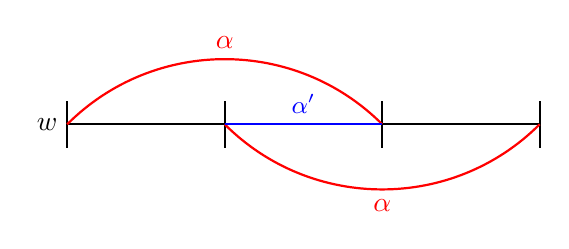
\begin{tikzpicture}
      \foreach \x in {0,2,4,6}{
        \coordinate (P\x) at (\x,0);
        \draw[thick] (P\x) -- ++(0,-0.3);
        \draw[thick] (P\x) -- ++(0,0.3);
      }
      
      \draw[thick] (P0) -- (P6);

      \node[left] at (P0) {\(w\)};
      \draw[thick, red, bend left=45] (P0) to node[midway, above, red] {\(\alpha\)} (P4);
      \draw[thick, red,bend right=45] (P2) to node[midway, below, red] {\(\alpha\)} (P6);

      \draw[thick, blue] (P2) to node[midway, above, blue,font=\small]{\(\alpha'\)} (P4);
    \end{tikzpicture}
  \end{figure}
  Infatti, poiché \(\abs{\alpha} > \frac{\abs{w}}{2}\) e \(\alpha\) è sia prefisso che suffisso di \(w\), necessariamente deve esistere una sovrapposizione \(\alpha'\) non vuota.
  Inoltre \(\alpha'\neq\alpha\), poiché essendo \(\alpha\) bordo dev'essere prefisso e suffisso proprio di \(w\) e l'unico caso in cui \(\alpha' = \alpha\) è quello in cui le due occorrenze di \(\alpha\) coincidono, portando a \(\alpha = w\).
  In più, com'è evidente dalla figura, \(\alpha'\) è sia prefisso che suffisso di \(\alpha\), dunque è un bordo di \(\alpha\).

  Ovviamente, un bordo di \(\alpha\) è anche un bordo di \(w\), poiché è sia prefisso di un prefisso di \(w\) che suffisso di un suffisso di \(w\).
  Inoltre, si ha che \(\abs{\alpha'} < \abs{\alpha}\), dunque, ripetendo questo ragionamento, si arriva necessariamente a un bordo \(\beta\) di \(w \st \abs{\beta} \leq \frac{\abs{w}}{2}\).
\end{proof}

Questo risultato ci suggerisce che per verificare che una parola ammetta bordi, è sufficiente verificare l'esistenza di bordi lunghi al più la metà della parola.

\begin{lemma}[label=lem:marcus-schutzenberger]{Marcus-Schützenberger}
  Sia \(X \subseteq A^+\) completo e non denso e \(\mu\) una distribuzione positiva su \(A\).
  Allora \(\mu(X) \geq 1\).
\end{lemma}
\begin{proof}
  Dato che \(X\) è non denso, esiste una parola \(w \in A^*\) che non si completa in \(X\).
  Sia \(y \in A^*\) qualsiasi.
  Poiché \(X\) è completo, la parola \(wyw\) si completa in \(X^*\), ovvero:
  \[\exists \lambda,\rho \in A^*\st \lambda w y w \rho  = x_1x_2\ldots x_n\in X^*\]
  \begin{figure}[H]
    \centering
    \begin{tikzpicture}
      \foreach \x in {0,2,4,6,8,10}{
        \coordinate (P\x) at (\x,0);
        \draw[thick] (P\x) -- ++(0,-0.3);
        \draw[thick] (P\x) -- ++(0,0.3);
      }
     
      \draw[thick] (P0) -- (P10);

      \node at ($(P0)!0.5!(P2)$) [below] {\(\lambda\)};
      \node at ($(P2)!0.5!(P4)$) [below] {\(w\)};
      \node at ($(P4)!0.5!(P6)$) [below] {\(y\)};
      \node at ($(P6)!0.5!(P8)$) [below] {\(w\)};
      \node at ($(P8)!0.5!(P10)$) [below] {\(\rho\)};

      \draw[thick, red, bend left=45] (P0) to node[midway, above, red] {\(x_1\)} (1,0);
      \draw[thick, red, bend left=45] (1,0) to node[midway, above, red] {\(x_2\)} (3,0);
      \draw[thick, red, bend left=45] (3,0) to node[midway, above, red] {\(x_i\)} (4.5,0);
      \draw[thick, red, bend left=45] (4.5,0) to (5.5,0);
      \draw[thick, red, bend left=45] (5.5,0) to  node[midway, above, red] {\(x_j\)} (6.5,0);
      \draw[thick, red, bend left=45] (6.5,0) to (7,0);
      \draw[thick, red, bend left=45] (7,0) to (9,0);
      \draw[thick, red, bend left=45] (9,0) to node[midway, above, red] {\(x_n\)} (P10);
    \end{tikzpicture}
  \end{figure}

  Poiché \(w\) non si completa in una parola di \(X\), allora nessuna delle occorrenze di \(w\) può essere contenuta interamente in una parola di \(X\).
  Dunque entrambe le occorrenze di \(w\) contengono almeno una \qi{linea di parsing} tra due parole di \(X\), ovvero un punto in cui termina una parola della fattorizzazione e inizia la seguente.
  Formalmente, esistono \(i,j \st 1 \leq i \leq j \leq n\) tali che \(x_i\) inizia all'interno della prima occorrenza di \(w\) e \(x_j\) termina all'interno della seconda occorrenza di \(w\).

  A questo punto notiamo che \(wyw \in Pref(w)\cdot X^* \cdot Suff(w)\), poiché $wyw$ corrisponde alla parte di $x_{2}$ (vedi figura) che sta nella prima occorrenza di $w$, una sequenza di parole di $X$ (in figura, $x_i\ldots x_{j+1}$), la parte di $x_{j+2}$ che sta nella seconda occorrenza di $w$. 
  Poiché \(y\) è arbitrario, si ha che \(\set{w}A^*\set{w} \subseteq Pref(w)\cdot X^* \cdot Suff(w)\)
  Dalle Proposizioni~\ref{prop:distribution_monotonicity} e~\ref{prop:distribution_distributivity_over_product}, segue che:
  \[\mu(\set{w}A^*\set{w}) \leq \mu(Pref(w)\cdot X^* \cdot Suff(w)) \leq \mu(Pref(w))\cdot \mu(X^*)\cdot \mu(Suff(w))\]
  Inoltre il prodotto \(\set{w}\times A^* \times \set{w}\) è chiaramente non ambiguo: dovrebbero esistere due triple distinte appartenenti a \(\set{w}\times A^* \times \set{w}\) corrispondenti alla stessa parola. L'unica parola che può variare in queste triple è il termine appartenente a $A^{*}$. Pertanto, due triple corrispondenti alla stessa parola devono essere uguali.
  Dunque dal viceversa della \Cref{prop:distribution_distributivity_over_product}, segue che:
  \[{\mu(\set{w})}^2\mu(A^*)=\mu(\set{w}A^*\set{w}) \leq \mu(Pref(w)\cdot X^* \cdot Suff(w)) \leq \mu(Pref(w))\cdot \mu(X^*)\cdot \mu(Suff(w))\]

  Poiché \(\mu\) è positiva, si ha che \({\mu(\set{w})}^2 > 0\), e dalla \Cref{prop:A_power_mesure_1} sappiamo che \(\mu(A^*) = \infty\).
  Dunque, per la disuguaglianza precedente, abbiamo che:
  \[\infty = {\mu(\set{w})}^2\mu(A^*) \leq \mu(Pref(w))\cdot \mu(X^*)\cdot \mu(Suff(w))\]
  E di conseguenza \(\mu(Pref(w))\cdot \mu(X^*)\cdot \mu(Suff(w)) = \infty\).
  Me essendo \(Pref(w)\) e \(Suff(w)\) finiti la loro misura è finita, dunque deve essere \(\mu(X^*) = \infty\).
  Abbiamo dunque dalla \Cref{prop:sub-additivity} che:
  \[\infty = \mu(X^*) = \mu(\bigcup_{k \geq 0}^{\infty} X^k) \leq \sum_{k \geq 0}^{\infty} \mu(X^k)\]
  Inoltre dalla \Cref{prop:distribution_distributivity_over_product}, segue che:
  \[\infty = \mu(X^*) = \mu(\bigcup_{k \geq 0}^{\infty} X^k) \leq \sum_{k \geq 0}^{\infty} \mu(X^k)\leq \sum_{k \geq 0}^{\infty} {\mu(X)}^k\]
  Dunque, $\mu(X^{*})$ è maggiorata da una serie geometrica divergente. Affinché una serie geometrica sia divergente, la sua ragione dev'essere maggiore o uguale a $1$. Quindi, \(\mu(X) \geq 1\).
\end{proof}

\begin{lemma}[label=lem:code_not_complete_boredless_word]{\infosymbol{} Estrapolato dalla dimostrazione del \Crefalt[yellow]{thm:schutz_maximality_completeness}}
  Sia \(X \subseteq A^+\) codice non completo, con \(\# A \geq 2\).
  Allora esiste una parola \(y \in A^*\) senza bordi che non si completa in \(X^*\).
\end{lemma}
\begin{proof}
  Poiché \(X\) non è completo, esiste una parola \(z \in A^*\) che non si completa in \(X^*\).
  Se tale parola non ha bordi, allora abbiamo trovato la parola cercata.
  Altrimenti, supponiamo che \(z\) abbia bordi e inizi per \(a \in A\).
  Poiché \(\# A \geq 2\), sia \(b \in A\setminus\set{a}\). Consideriamo la parola \(y = zb^{\abs{z}}\).
  Tale parola non può completarsi in \(X^*\): se $y$ si completasse in $X^{*}$, allora anche $z \in Pref(y)$ si completerebbe in $X^{*}$, ma ciò è impossibile per come abbiamo scelto $z$.
  Notiamo che la prima metà di $y$ è costituita da $z$, che inizia per $a\in A$, mentre la seconda metà è costituita da una sequenza di $b$. Quindi per $y$ non possono esistere bordi di lunghezza \(\leq\frac{\abs{y}}{2} = \abs{z}\). La Proposizione~\ref{prop:if_border_exists_border_half_length} ci assicura che, allora, per $y$ non esistono bordi.
\end{proof}

A questo punto siamo in grado di dimostrare il Teorema di Schützenberger~\ref{thm:schutz_maximality_completeness}.
\begin{proof}[Dimostrazione di~\ref{thm:schutz_maximality_completeness}]
  \begin{enumerate}
    \item Per dimostrare che se \(X\) è massimale allora è completo, procediamo per contrapposizione, ovvero assumendo che \(X\) non sia completo e mostrando che in tal caso non può essere massimale.
      Iniziamo escludendo il caso banale in cui \(\# A = 1\). In questo casi infatti, tutti i codici possibili sono singleton, poiché ogni altro insieme di parole porta a parole con plurime fattorizzazioni\footnote{Si prenda ad esempio \(Z = \set{a^k,a^h}\). In tal caso \(a^{h+k} = a^h a^k = a^k a^h\)}.
      Di conseguenza tutti i codici sono massimali, e sono inoltre anche completi, poiché ogni parola \(a^m\) si completa in \(X = \set{a^h}\) aggiungendo a \(a^m\) tante \(a\) fino a raggiungere un multiplo di \(h\).

      Sia dunque \(\# A \geq 2\) e sia \(y \in A^*\) che non si completa in \(X^*\) (esistenza garantita dal fatto che \(X\) è assunto non completo).
      Possiamo scegliere senza perdita di generalità \(y\) senza bordi dal \Cref{lem:code_not_complete_boredless_word}.

      Consideriamo il linguaggio \(Y=X\cup\set{y}\). Vogliamo dimostrare che $Y$ è codice, ovvero che è $X$ non è massimale.
      Supponiamo dunque per assurdo che $Y$ \textbf{non} sia codice.
      Allora esiste una parola di \(Y^*\) con multipla fattorizzazione, ovvero esistono \(y_1,y_2,\ldots y_m,y_1',y_2',\ldots,y_n' \in Y\) tali che \(y_1y_2\ldots y_m = y_1y_2\ldots y_n'\), con \(y_1\neq y_1'\).
      Tra queste parole deve necessariamente esserci almeno una occorrenza di \(y\), poiché altrimenti tale parola apparterrebbe a \(X^*\), contraddicendo l'ipotesi che \(X\) è codice.
      Inoltre, poiché \(y\) non si completa in \(X^*\), dev'esserci almeno un occorrenza di \(y\) in entrambe le fattorizzazioni. Infatti:
      \begin{itemize}
        \item se non comparisse in nessuna delle due fattorizzazioni, allora avremmo trovato una doppia fattorizzazione con soli elementi di $X$, ovvero $X$ non dovrebbe essere codice;
        \item se comparisse in una sola fattorizzazione, allora, affinché le due fattorizzazioni siano uguali, $y$ dovrebbe completarsi in una parola di $x$, ma $y$ non si completa in $X$.
      \end{itemize}
      Dunque \(\exists i,j \st y_i=y_j'=y\). Scegliamo senza perdita di generalità \(i\) e \(j\) minimi con tale proprietà.

      Analizziamo dunque per casi i possibili posizionamenti delle due occorrenze di \(y\) nelle due fattorizzazione sovrapposte:
      \begin{description}
        \item[Le due occorrenze di \(y\) non hanno sovrapposizione]
          In questo caso, è possibile rappresentare le due fattorizzazioni come segue:
          \begin{figure}[H]
            \centering
            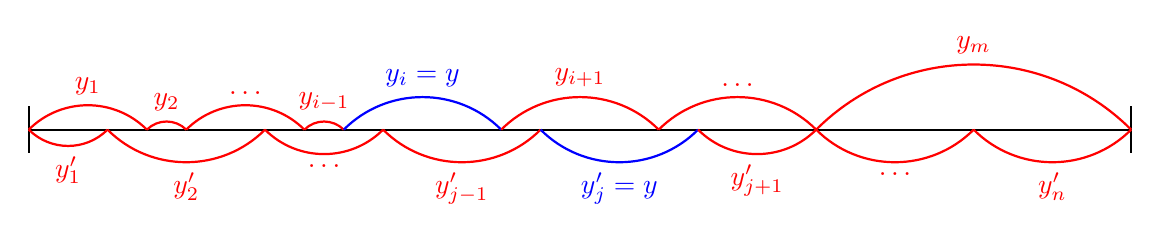
\begin{tikzpicture}
              \foreach \x in {0,2,4,6,8,10,12,14}{
                \coordinate (P\x) at (\x,0);
              }
             
              \draw[thick] (P0) -- ++(0,-0.3);
              \draw[thick] (P0) -- ++(0,0.3);
              \draw[thick] (P14) -- ++(0,-0.3);
              \draw[thick] (P14) -- ++(0,0.3);
              \draw[thick] (P0) -- (P14);

              \draw[thick, red, bend left=45] (P0) to node[midway, above, red] {\(y_1\)} (1.5,0);
              \draw[thick, red, bend left=45] (1.5,0) to node[midway, above, red] {\(y_2\)} (2,0);
              \draw[thick, red, bend left=45] (2,0) to node[midway, above, red] {\(\ldots\)} (3.5,0);
              \draw[thick, red, bend left=45] (3.5,0) to node[midway, above, red] {\(y_{i-1}\)} (4,0);
              \draw[thick, blue, bend left=45] (4,0) to node[midway, above, blue] {\(y_i = y\)} (6,0);
              \draw[thick, red, bend left=45] (6,0) to node[midway, above, red] {\(y_{i+1}\)} (P8);
              \draw[thick, red, bend left=45] (P8) to node[midway, above, red] {\(\ldots\)} (P10);
              \draw[thick, red, bend left=45] (P10) to node[midway, above, red] {\(y_m\)} (P14);

              \draw[thick, red, bend right=45] (P0) to node[midway, below, red] {\(y_1'\)} (1,0);
              \draw[thick, red, bend right=45] (1,0) to node[midway, below, red] {\(y_2'\)} (3,0);
              \draw[thick, red, bend right=45] (3,0) to node[midway, below, red] {\(\ldots\)} (4.5,0);
              \draw[thick, red, bend right=45] (4.5,0) to node[midway, below, red] {\(y_{j-1}'\)} (6.5,0);
              \draw[thick, blue, bend right=45] (6.5,0) to node[midway, below, blue] {\(y_j' = y\)} (8.5,0);
              \draw[thick, red, bend right=45] (8.5,0) to node[midway, below, red] {\(y_{j+1}'\)} (P10);
              \draw[thick, red, bend right=45] (P10) to node[midway, below, red] {\(\ldots\)} (P12);
              \draw[thick, red, bend right=45] (P12) to node[midway, below, red] {\(y_n'\)} (P14);
            \end{tikzpicture}
          \end{figure}
          In questo caso però, sarebbe possibile completare \(y\) in \(X^*\), poiché la parola \(y_1'y_2'\ldots y_{j-1}'\) appartiene a \(X^*\) per minimalità di \(j\), e contiene \(y\) come sottoparola. Assurdo!
          \item[Le due occorrenze di \(y\) hanno sovrapposizione parziale]
          In questo caso, è possibile rappresentare le due fattorizzazioni come segue:
          \begin{figure}[H]
            \centering
            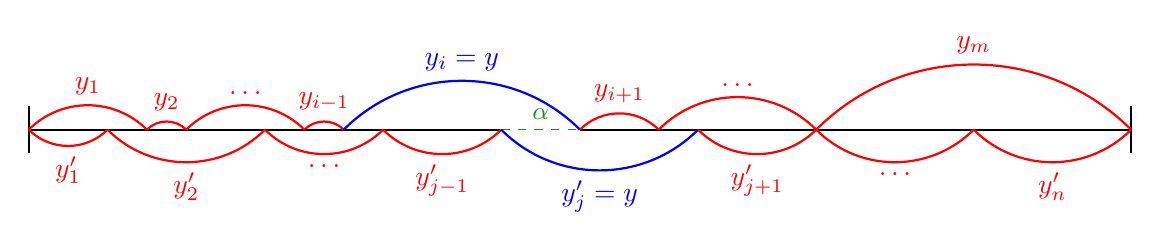
\begin{tikzpicture}
              \foreach \x in {0,2,4,6,8,10,12,14}{
                \coordinate (P\x) at (\x,0);
              }
             
              \draw[thick] (P0) -- ++(0,-0.3);
              \draw[thick] (P0) -- ++(0,0.3);
              \draw[thick] (P14) -- ++(0,-0.3);
              \draw[thick] (P14) -- ++(0,0.3);
              \draw[thick] (P0) -- (P14);

              \draw[thick, white] (6,0) to (7,0);
              \draw[dashed, ForestGreen] (6,0) to node[midway, above=0.01pt, ForestGreen,font=\small]{\(\alpha\)} (7,0);

              \draw[thick, red, bend left=45] (P0) to node[midway, above, red] {\(y_1\)} (1.5,0);
              \draw[thick, red, bend left=45] (1.5,0) to node[midway, above, red] {\(y_2\)} (2,0);
              \draw[thick, red, bend left=45] (2,0) to node[midway, above, red] {\(\ldots\)} (3.5,0);
              \draw[thick, red, bend left=45] (3.5,0) to node[midway, above, red] {\(y_{i-1}\)} (4,0);
              \draw[thick, blue, bend left=45] (4,0) to node[midway, above, blue] {\(y_i = y\)} (7,0);
              \draw[thick, red, bend left=45] (7,0) to node[midway, above, red] {\(y_{i+1}\)} (P8);
              \draw[thick, red, bend left=45] (P8) to node[midway, above, red] {\(\ldots\)} (P10);
              \draw[thick, red, bend left=45] (P10) to node[midway, above, red] {\(y_m\)} (P14);

              \draw[thick, red, bend right=45] (P0) to node[midway, below, red] {\(y_1'\)} (1,0);
              \draw[thick, red, bend right=45] (1,0) to node[midway, below, red] {\(y_2'\)} (3,0);
              \draw[thick, red, bend right=45] (3,0) to node[midway, below, red] {\(\ldots\)} (4.5,0);
              \draw[thick, red, bend right=45] (4.5,0) to node[midway, below, red] {\(y_{j-1}'\)} (6,0);
              \draw[thick, blue, bend right=45] (6,0) to node[midway, below, blue] {\(y_j' = y\)} (8.5,0);
              \draw[thick, red, bend right=45] (8.5,0) to node[midway, below, red] {\(y_{j+1}'\)} (P10);
              \draw[thick, red, bend right=45] (P10) to node[midway, below, red] {\(\ldots\)} (P12);
              \draw[thick, red, bend right=45] (P12) to node[midway, below, red] {\(y_n'\)} (P14);

            \end{tikzpicture}
          \end{figure}
          Tale sovrapposizione è indicata in verde nella figura come \(\alpha\).
          Essendo però \(\alpha\) sia suffisso di \(y\) (essendo parte della occorrenza \(i\) di \(y\)) che prefisso di \(y\) (essendo parte della occorrenza \(j\) di \(y\)), e non essendo \(\alpha = y\) (poiché le due occorrenze di \(y\) non coincidono), si ha che \(\alpha\) è un bordo di \(y\), contraddicendo l'ipotesi che \(y\) non abbia bordi. Assurdo!
        \item[Le due occorrenze di \(y\) sono allineate]
          Infine, consideriamo il caso in cui le due occorrenze di \(y\) siano allineate, ovvero:
          \begin{figure}[H]
            \centering
            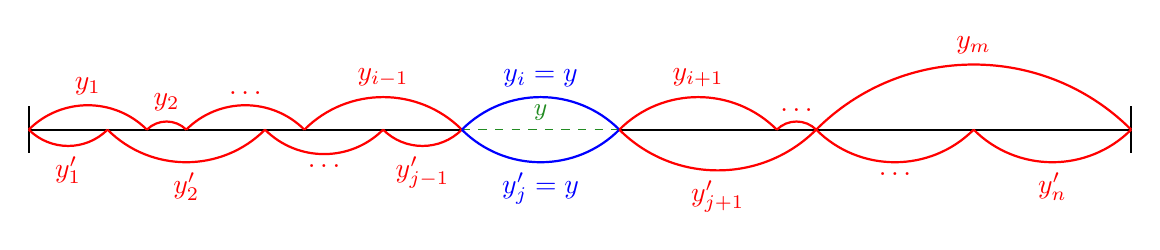
\begin{tikzpicture}
              \foreach \x in {0,2,4,6,8,10,12,14}{
                \coordinate (P\x) at (\x,0);
              }
             
              \draw[thick] (P0) -- ++(0,-0.3);
              \draw[thick] (P0) -- ++(0,0.3);
              \draw[thick] (P14) -- ++(0,-0.3);
              \draw[thick] (P14) -- ++(0,0.3);
              \draw[thick] (P0) -- (P14);

              \draw[thick, white] (5.5,0) to (7.5,0);
              \draw[dashed, ForestGreen] (5.5,0) to node[midway, above=0.01pt, ForestGreen,font=\small]{\(y\)} (7.5,0);

              \draw[thick, red, bend left=45] (P0) to node[midway, above, red] {\(y_1\)} (1.5,0);
              \draw[thick, red, bend left=45] (1.5,0) to node[midway, above, red] {\(y_2\)} (2,0);
              \draw[thick, red, bend left=45] (2,0) to node[midway, above, red] {\(\ldots\)} (3.5,0);
              \draw[thick, red, bend left=45] (3.5,0) to node[midway, above, red] {\(y_{i-1}\)} (5.5,0);
              \draw[thick, blue, bend left=45] (5.5,0) to node[midway, above, blue] {\(y_i = y\)} (7.5,0);
              \draw[thick, red, bend left=45] (7.5,0) to node[midway, above, red] {\(y_{i+1}\)} (9.5,0);
              \draw[thick, red, bend left=45] (9.5,0) to node[midway, above, red] {\(\ldots\)} (P10);
              \draw[thick, red, bend left=45] (P10) to node[midway, above, red] {\(y_m\)} (P14);

              \draw[thick, red, bend right=45] (P0) to node[midway, below, red] {\(y_1'\)} (1,0);
              \draw[thick, red, bend right=45] (1,0) to node[midway, below, red] {\(y_2'\)} (3,0);
              \draw[thick, red, bend right=45] (3,0) to node[midway, below, red] {\(\ldots\)} (4.5,0);
              \draw[thick, red, bend right=45] (4.5,0) to node[midway, below, red] {\(y_{j-1}'\)} (5.5,0);
              \draw[thick, blue, bend right=45] (5.5,0) to node[midway, below, blue] {\(y_j' = y\)} (7.5,0);
              \draw[thick, red, bend right=45] (7.5,0) to node[midway, below, red] {\(y_{j+1}'\)} (P10);
              \draw[thick, red, bend right=45] (P10) to node[midway, below, red] {\(\ldots\)} (P12);
              \draw[thick, red, bend right=45] (P12) to node[midway, below, red] {\(y_n'\)} (P14);

            \end{tikzpicture}
          \end{figure}
          In tale situazione però si avrebbe che \(y_1y_2\ldots y_{i+1} = y_1'y_2'\ldots y_{j-1}'\) è una doppia fattorizzazione di una parola ottenuta concatenando parole di \(X\), dalla minimalità di \(i\) e \(j\). Dunque questo contraddice l'ipotesi che \(X\) sia codice. Assurdo!
      \end{description}
      L'assunzione dunque che esista una doppia fattorizzazione in \(Y\), e che quindi non sia codice, porta a una contraddizione in ogni possibile caso.
      Di conseguenza, dato \(X\) non completo, è sempre possibile costruire un sovrainsieme \(Y\) che è ancora codice, mostrando che \(X\) non è massimale.
      Ergo, per contrapposizione, se \(X\) è massimale allora è completo.
    \item In questo caso, sappiamo per ipotesi che \(X\) è completo e non denso.
      Dunque presa \(\mu\) distribuzione positiva su \(A\), dal \Cref{lem:marcus-schutzenberger} sappiamo che \(\mu(X) \geq 1\).
      D'altra parte, dal \Cref{thm:kraft-mcmillan}, sappiamo che \(\mu(X) \leq 1\), poiché \(X\) è codice.
      Dunque, si ha che \(\mu(X) = 1\). Come visto in precedenza, ciò implica che \(X\) è massimale.
  \end{enumerate}
\end{proof}

\begin{observation}{}
  L'ipotesi \emph{non denso} nel secondo punto del \Cref{thm:schutz_maximality_completeness} è necessaria. Infatti il codice \(Z = \{a^{|u|+1}bu | u \in {\{a,b\}}^*\}\) è un codice denso (e quindi completo), ma non massimale.
  Infatti \(Z\cup\{b\}\) è ancora un codice (prefisso).
\end{observation}

Un diretto corollario del Teorema di Schützenberger è il seguente:
\begin{corollary}[label=cor:schutz_maximality_completeness]{}
  Sia \(X \subseteq A^+\) codice non denso. Allora le seguenti affermazioni sono equivalenti:
  \begin{enumerate}
    \item \(X\) è massimale
    \item \(X\) è completo
    \item \(\forall \mu\) distribuzione positiva su \(A\): \(\mu(X) = 1\)
    \item \(\exists \mu\) distribuzione positiva su \(A\): \(\mu(X) = 1\)
  \end{enumerate}
\end{corollary}
\begin{proof}
  Si ha che \(1 \iff 2\) per il punto \(1\) del \Cref{thm:schutz_maximality_completeness}, \(2 \implies 3\) viene dalla dimostrazione del punto \(2\) del \Cref{thm:schutz_maximality_completeness} per via della massimalità, \(3 \implies 4\) è banale e \(4 \implies 1\) è stato più volte dimostrato precedentemente.
\end{proof}

Vediamo dunque alcune proposizioni che seguono dai risultati appena dimostrati.

\begin{proposition}{}
  Sia \(X\subseteq A^*\) finito e completo, e \(\mu\) distribuzione positiva su \(A\) tale che \(\mu(X) = 1\). Allora \(X\) è un codice. Inoltre, $X$ è massimale.
\end{proposition}

\begin{proof}
  \(\forall n \geq 1, X^n\) è completo. Infatti se \(w\) si completa in \(X^*\) allora si completa anche in \({(X^n)}^*\).
  Essendo \(X\) finito, anche \(X^n\) è finito, e di conseguenza è anche non denso. Dunque per il \Cref{lem:marcus-schutzenberger} si ha che:
  \[1\leq \mu(X^n) \leq {\mu(X)}^n = 1^n = 1\]
  Quindi \(\forall n \geq 1: \mu(X^n) = 1 = {\mu(X)}^n\).
  Di conseguenza, per il viceversa della \Cref{prop:code_implies_equal_mesures_of_powers} si ha che \(X\) è un codice.
  Inoltre, poiché $\mu(X)=1$, allora $X$ è massimale.
\end{proof}

\begin{proposition}[label=prop:finite_complete_codes_contains_powers]{}
  Sia \(X \subseteq A^*\) finito e completo. Allora \(\forall a \in A \exists n \geq 1 : a^n \in X\). Inoltre, se $X$ è codice, tale \(n\) è unico.
\end{proposition}

\begin{proof}
  Essendo \(X\) finito esiste una lunghezza di parola massima.
  Sia dunque \(L = \max_{x \in X}\abs{x}\) e \(a \in A\).
  Essendo \(X\) completo, \(a^{2L}\) si completa in \(X^*\), quindi esistono \(\lambda, \rho \in A^*: \lambda a^{2L} \rho \in X^*\).
  \begin{figure}[H]
    \centering
    \begin{tikzpicture}
      \foreach \x in {0,2,4,6,8,10}{
        \coordinate (P\x) at (\x,0);
      }
      
      \draw[thick] (P0) -- ++(0,-0.3);
      \draw[thick] (P0) -- ++(0,0.3);
      \draw[thick] (P2) -- ++(0,-0.3);
      \draw[thick] (P2) -- ++(0,0.3);
      \draw[thick] (P8) -- ++(0,-0.3);
      \draw[thick] (P8) -- ++(0,0.3);
      \draw[thick] (P10) -- ++(0,-0.3);
      \draw[thick] (P10) -- ++(0,0.3);
      \draw[thick] (P0) -- (P10);

      \node at ($(P0)!0.5!(P2)$) [above] {\(\lambda\)};
      \node at ($(P2)!0.5!(P8)$) [above] {\(a^{2L}\)};
      \node at ($(P8)!0.5!(P10)$) [above] {\(\rho\)};

      \draw[thick, red, bend right=45] (P0) to node[midway, below, red] {\(x_1\)} (1,0);
      \draw[thick, red, bend right=45] (1,0) to node[midway, below, red] {\(x_2\)} (3,0);
      \draw[thick, red, bend right=45] (3,0) to node[midway, below, red] {\(\ldots\)} (4.5,0);
      \draw[thick, red, bend right=45] (4.5,0) to node[midway, below, red] {\(x_i\)} (5.5,0);
      \draw[thick, red, bend right=45] (5.5,0) to node[midway, below, red] {\(\ldots\)} (7.5,0);
      \draw[thick, red, bend right=45] (7.5,0) to node[midway, below, red] {\(x_m\)} (P10);

    \end{tikzpicture}
  \end{figure}
  Poiché ogni parola in \(X\) ha lunghezza al più \(L\), esiste un \(x_i\) della fattorizzazione di \(\lambda a^{2L} \rho\) che è sottoparola propria di \(a^{2L}\). Infatti, se così non fosse si avrebbero due parole \(x_i,x_{i+1}\in X\) adiacenti tali per cui $x_i x_{i+1}$ inizia in $\lambda$ e finisce in $\rho$, ottenendo la seguente rappresentazione:
    \begin{figure}[H]
    \centering
    \begin{tikzpicture}
      \foreach \x in {0,2,4,6,8,10}{
        \coordinate (P\x) at (\x,0);
      }
      
      \draw[thick] (P0) -- ++(0,-0.3);
      \draw[thick] (P0) -- ++(0,0.3);
      \draw[thick] (P2) -- ++(0,-0.3);
      \draw[thick] (P2) -- ++(0,0.3);
      \draw[thick] (P8) -- ++(0,-0.3);
      \draw[thick] (P8) -- ++(0,0.3);
      \draw[thick] (P10) -- ++(0,-0.3);
      \draw[thick] (P10) -- ++(0,0.3);
      \draw[thick] (P0) -- (P10);

      \node at ($(P0)!0.5!(P2)$) [above] {\(\lambda\)};
      \node at ($(P2)!0.5!(P8)$) [above] {\(a^{2L}\)};
      \node at ($(P8)!0.5!(P10)$) [above] {\(\rho\)};

      \draw[thick, red, bend right=45] (P0) to node[midway, below, red] {\(x_1\)} (0.5,0);
      \draw[thick, red, bend right=45] (0.5,0) to node[midway, below, red] {\(x_2\)} (1,0);
      \draw[thick, red, bend right=45] (1,0) to node[midway, below, red] {\(\ldots\)} (1.5,0);
      \draw[thick, red, bend right=45] (1.5,0) to node[midway, below, red] {\(x_i\)} (5,0);
      \draw[thick, red, bend right=45] (5,0) to node[midway, below, red] {\(x_{i+1}\)} (8.5,0);
      \draw[thick, red, bend right=45] (8.5,0) to node[midway, below, red] {\(\ldots\)} (9,0);
      \draw[thick, red, bend right=45] (9,0) to node[midway, below, red] {\(x_m\)} (P10);

    \end{tikzpicture}
  \end{figure}
  Ma allora si osserverebbe \(\abs{x_i x_{i+1}} = \abs{x_i} + \abs{x_{i+1}} > 2L\), implicando che almeno una delle due parole ha lunghezza maggiore di \(L\). Assurdo!
  
  Da ciò segue che tale \(x_i\) è della forma \(a^n\).
  Inoltre, se \(X\) è codice, \(n\) è unico: se esistesse \(m\neq n\) tale che \(a^m \in X\), allora la parola \(a^{n+m}\) avrebbe due fattorizzazioni distinte in \(X^*\), portando ad un assurdo.
\end{proof}

\begin{definition}{Completamento di un codice}
  Sia \(X \subseteq A^*\) un codice.
  Un \emph{completamento} di \(X\) è un codice \(Y \supseteq X\) sullo stesso alfabeto che sia massimale.

  In altre parole, un completamento di un codice \(X\) è un sovrainsieme di \(X\) massimale rispetto alla proprietà di essere codice.
\end{definition}
Da questa definizione sorgono alcune domande riguardo alla completabilità dei codici:
\begin{enumerate}
  \item Dato un codice \(X\) qualsiasi, esiste sempre un completamento?
    Tale quesito ha risposta affermativa, e ne vedremo la dimostrazione più avanti.
  \item Dato un codice \(X\) finito, esiste sempre un completamento finito?
    In questo caso la risposta è negativa.
    Un esempio noto fornito da Markov ha mostrato che dato \(A = \set{a,b}\), il codice \(X = \set{a^5,ab,ba^2,b}\) non ha completamenti finiti.
  \item A questo punto, \emph{quali} codici finiti ammettono completamento finito?
    In generale, la caratterizzazione completa è un problema aperto, ma:
    \begin{itemize}
      \item I codici finiti prefissi ammettono sempre completamenti finiti.
        Caso particolare di questo caso qualsiasi codice finito con cardinalità \(1\) ammette sempre completamento finito.
      \item Se \(\#X = 2\), allora \(X\) ammette un completamento finito, dimostrato da Restivo.
      \item Se \(\#X \geq 4\), in generale non ammette un completamento finito. Infatti l'esempio di Markov ha cardinalità \(4\).
      \item Se \(\#X = 3\), il problema è aperto.
    \end{itemize}
\end{enumerate}


Vediamo dunque la dimostrazione dell'esistenza di un completamento per ogni codice citato in precedenza.
\begin{proposition}{}
  Sia \(X \subseteq A^*\) codice. Allora esiste un completamento di \(X\).
\end{proposition}
La proposizione afferma che per ogni $X$ esiste un completamento, finito o infinito.
\begin{proof}
  Se \(X\) è massimale, allora \(X\), che denotiamo con \(X_{0}\) è un completamento di sé stesso.
  Altrimenti, esiste \(w_1 \in A^*\setminus X\) di lunghezza minima tale che \(X_1 = X_0 \cup \{w_1\}\) è ancora un codice.
  Se \(X_1\) è massimale, abbiamo finito.
  In generale, se iterando questo procedimento otteniamo \(X_k = X_{k-1} \cup \set{w_k}\) massimale, abbiamo finito.
  Altrimenti, otteniamo una successione infinita di parole \(s = \set{w_n}\). Vogliamo mostrare che \(Y = \bigcup_{k = 0}^{\infty} X_k\), ottenuto applicando il procedimento, è un codice massimale.
  $Y$ è codice, infatti: per assurdo $Y$ non è codice, quindi esiste una doppia fattorizzazione $x_{1}\ldots x_{i}=x_{1}'\ldots x_{j}'$ con $x_{1}\neq x_{1}'$. Vi sarà un $k$ t.c. $X_k$ contiene tutti gli elementi della doppia fattorizzazione. Quindi, $X_k$ non è codice. Assurdo!\\
  $Y$ è anche massimale: per assurdo, esiste un \(w \in A^* \setminus Y\) tale che \(Y \cup \{w\}\) è ancora un codice. Allora, esiste sicuramente un \(m\) tale che \(\abs{w_m} > \abs{w}\), poiché, aggiungendo parole all'infinito, dovranno essere state aggiunte, secondo il procedimento, tutte le parole di lunghezza minore o uguale a $\abs{w}$. Ma, allora, il procedimento, al passo $m$, avrebbe scelto un $w_m$ non minimo. Assurdo!
\end{proof}

Con quest'ultimo risultato, si conclude la trattazione delle proprietà algebriche dei codici, che ci serviranno come presupposti teorici per la trattazione della codifica di sorgente nel capitolo successivo, che si addentrerà maggiormente sugli aspetti legati alla teoria dell'informazione.
\chapter{Codifica di Sorgente}

Ci inoltriamo finalmente nel cuore della teoria dell'informazione, ovvero la codifica di sorgente.

\section{Sorgenti e Codifica}

\begin{definition}{Sorgente (discreta e a memoria zero)}
  Chiamiamo \keyword{Sorgente discreta e a memoria zero} una variabile aleatoria discreta, identificabile come una coppia \(S = (\SCal,p)\), con \(\SCal\) alfabeto finito, e \(p\) distribuzione su \(\SCal\).
\end{definition}
$\SCal$ viene spesso detto \textit{alfabeto sorgente}.

\begin{definition}{Codifica}
  Definiamo \keyword{codifica} un morfismo iniettivo \(\varphi: \SCal^* \to A^*\) con \(A\) alfabeto. Il morfismo $\varphi$ identifica il \keyword{codice} $X=\varphi(\SCal)$.
  Diremo inoltre che $X$ è \keyword{adattabile} alla sorgente \(S\) se \(\# X = \# \SCal\).
  In particolare, $X$ sarà \keyword{adattato} a una sorgente \(S\) mediante \(\varphi\), se \(\varphi\) induce una biezione tra \(\SCal\) e \(X\), \(\varphi_{|_X}: \SCal \leftrightarrow X\).
\end{definition}
Si noti che il fatto che un $X$ sia adattabile non implica che esso sia anche adattato: l'esistenza di una biezione tra $X$ e $\SCal$ non è garantita da $\#\SCal=\#X$. Ciò avviene perché $\varphi$ è definito come iniettivo: $\varphi$ potrebbe non mappare una parola di $X$. Invece, nel caso in cui $\varphi$ mappi tutte le parole di $X$, allora si può ottenere la biezione $\varphi_{|_X}$ semplicemente restringendo $\varphi$ a $\varphi^{-1}(X)$, ovvero forzando la suriettività.

\begin{definition}{Costo di una codifica}
  Data una sorgente \(S = (\SCal,p)\) e una codifica \(\varphi: \SCal^* \to A^*\) con codice \(X = \varphi(\SCal)\), definiamo il \keyword{costo} di \(\varphi\) la quantità:
  \[c(X,\varphi) = \sum_{s \in \SCal} p(s) \abs{\varphi(s)}\]
  ovvero la media pesata sulla distribuzione \(p\) delle lunghezze delle parole codificate.\\
  Il \keyword{costo assoluto} di un codice \(X\) sarà
  \[c(X) = \min_{\varphi: \varphi(\SCal) \leftrightarrow  X} c(X,\varphi)\] ovvero il costo associato alla codifica che per cui si ottiene il costo minimo.
\end{definition}

\begin{example}[label=ex:codifica]{}
  Sia \(\SCal = \set{s_1,s_2,s_3}\), \(A = \set{a,b}\), \(X = \set{a,ba,bb}\).
  Se \(p(s_1) = 1/2, p(s_2) = p(s_3) = 1/4\), e inoltre \(\varphi(s_1) = ba, \varphi(s_2) = a, \varphi(s_3) = bb\), si ha che
    \[c(X,\varphi) = \frac{7}{4} > c(X) = \frac{3}{2}\]
  dove $c(X)$ è il costo ottenuto scegliendo la codifica $\varphi'$ che associa probabilità maggiori a parole di $X$ più corte, ovvero associa la probabilità massima alla parola più corta, la seconda probabilità massima alla seconda parola più corta e così via. 
\end{example}

La scelta di $\varphi'$ nell'esempio non è casuale, ma è anzi il risultato della seguente proposizione.

\begin{proposition}{}
  Sia \(S\) sorgente, \(X\) codice su \(A\) \emph{adattato} a \(S\) mediante \(\varphi\).
  Allora \(c(X) = c(X,\varphi)\) se e solo se
    \[\forall s,s' \in \SCal, p(s) < p(s') \implies \abs{\varphi(s)} < \abs{\varphi(s')} \]
\end{proposition}

\begin{definition}{Codice ottimale}
  Diremo che \(X\) è un \keyword{codice ottimale} per la sorgente \(S\) se, per ogni codice \(Z\) sullo stesso alfabeto e con la stessa cardinalità, si ha che
  \[c(X) \leq c(Z)\]
\end{definition}

In altre parole, un codice è ottimale se il suo costo assoluto è minore o uguale di qualsiasi altro costo assoluto ottenuto a partire da un altro codice sullo stesso alfabeto e con stessa cardinalità.

\begin{example}{}
  Data la sorgente dell'esempio~\ref{ex:codifica}, il codice \(Z = \set{aa,ba,bb}\) \textbf{non} è ottimale, poiché \(c(Z) = 2\), mentre abbiamo trovato un codice di costo inferiore nell'esempio precedente.
\end{example}

\section{Entropia di una sorgente}

\begin{definition}{Entropia di una sorgente}
  Data una sorgente \(S = (\SCal,p)\), definiamo l'\keyword{entropia} di \(S\) la quantità
  \[H(S) = -\sum_{s \in \SCal} p(s) \log\left(p(s)\right) = \sum_{s \in \SCal} p(s) \log\left(\frac{1}{p(s)}\right)\]  
\end{definition}

Tale quantità rappresenta un valore medio dell'autoinformazione (ovvero dell'incertezza) della sorgente.
La base del logaritmo non è specificata in quanto cambierebbe il valore di $H(S)$ solo di una costante moltiplicativa dovuta al cambio di base. Tale costante moltiplicativa è del tutto analoga ad un cambio di unità di misura.

Infatti, l'entropia (e l'informazione in generale) si misura utilizzando comunemente tre unità di misura:
\begin{itemize}
  \item \emph{hartley} (base \(10\)), prima unità di misura dell'informazione;
  \item \emph{nat} (base \(e\)), utile per alcune formulazioni matematiche;
  \item \emph{bit} (base \(2\)), più utilizzata al giorno d'oggi.
\end{itemize}
L'entropia di \(1 bit\) è quella di una sorgente binaria uniforme:
\[H(S) = \frac{1}{2}\log_2(2) + \frac{1}{2}\log_2(2) = 1\]
Da questo momento in avanti si farà riferimento unicamente ai \(bit\) come unità di misura dell'informazione, omettendo dunque la base del logaritmo e assumendola pari a $2$.

\begin{note}[label=note:entropy-continuity-assumption]{}
  La definizione di entropia fornita non esclude la possibilità di avere \(p(s) = 0\) per qualche \(s \in \SCal\).
  In tal caso il termine della somma corrispondente a tale \(s\) non sarebbe definito, in quanto si otterrebbe una forma indeterminata $0\cdot -\infty$.
  Dunque, per fornire continuità a $H$, si assume \(p(s)\log\left(p(s)\right) = 0\), dato che è noto che \(\lim_{x \to 0^+} x \log\left(x\right) = 0\).

  In maniera formale, si può ridefinire l'entropia come
  \[H(S) = -\sum_{s \in \SCal} h(s)\]
  dove
  \[h(s) = \begin{cases}
              p(s) \log\left(p(s)\right) & , p(s) > 0 \\
              0 & , p(s) = 0
            \end{cases}
  \]
\end{note}

Andiamo adesso a dimostrare che l'entropia è sempre dotata di un limite inferiore e di un limite superiore.

\begin{proposition}[label=prop:lower_bound_entropy]{Limite inferiore dell'entropia}
  Sia $S=(\mathcal{S},p)$ una sorgente discreta a memoria zero. Allora si ha $H(S)\geq 0$.\\
  Inoltre, $H(S)=0 \iff \exists !\bar{s}\in \mathcal{S}:p(s)=1$.
\end{proposition}

\begin{proof}
  Poiché \(\forall s \in \SCal: 0\leq p(s) \leq 1\), abbiamo che\footnote{È denotato che \(-\infty \leq \log\left(p(s)\right)\) e non \(-\infty < \log\left(p(s)\right)\), poiché si assume \(\log\left(0\right)\) definito come \(-\infty\) per continuità.}
  \[-\infty \leq \log\left(p(s)\right) \leq 0 \iff  0 \leq -\log\left(p(s)\right) = \log\left(\frac{1}{p(s)}\right) \leq \infty\]

  Dunque \(H(S) = \sum_{s \in \SCal} p(s) \log\left(\frac{1}{p(s)}\right) = \mathbb{E}[\log\left(\frac{1}{p(S)}\right)] \geq 0\), essendo somma pesata di quantità non negative.

  Inoltre, se \(p(s) = 1\) e \(p(t) = 0, \forall t \in \SCal \setminus \set{s}\) si ha che
  \[H(S) = 1 \cdot \log\left(\frac{1}{1}\right) - \sum_{t \in \SCal \setminus \set{s}} 0 \cdot \log\left(0\right) = 0 - 0 = 0\]
  Viceversa, se \(H(S) = 0\), deve aversi \(p(s) \log\left(\frac{1}{p(s)}\right) = 0, \forall s \in \SCal\), che può avvenire solo in due casi, ovvero \(\forall s \in \SCal (p(s) = 0 \lor p(s) = 1)\).
  Poiché \(p\) è una distribuzione di probabilità, si ha \(\sum_{s \in \SCal} p(s) = 1\), e dunque
  \[\exists!\bar{s} \in \SCal: p(\bar{s}) = 1\]
\end{proof}

\begin{proposition}[label=prop:upper_bound_entropy]{Limite superiore dell'entropia}
  Sia $S=(\mathcal{S},p)$ una sorgente discreta a memoria zero e $k=\#\mathcal{S}$. Allora si ha $H(S)\leq \log k$.\\
  Inoltre, $H(S)=\log k \iff \forall s \in \mathcal{S}:p(s)=\frac{1}{k}$.
\end{proposition}

Per dimostrare questa proposizione, abbiamo bisogno di un risultato di Analisi matematica: la disuguaglianza di Gibbs.

Siano $p,q$ distribuzioni su $\mathcal{S}$. Allora:
\begin{equation}\label{eq:gibbs}
H(S)=\sum_{s \in \mathcal{S}}{p(s)\log\left( \frac{1}{p(s)} \right)} \leq \sum_{s \in \mathcal{S}}{p(s)\log\left( \frac{1}{q(s)} \right)}
\end{equation}
e vale con il segno uguale solo se $p=q$.

\begin{note}{}
  Si noti che la somma a destra può divergere, poiché non vale l'assunzione \ref{note:entropy-continuity-assumption} in quanto i due termini della somma appartengono a due distribuzioni distinte. Infatti, potrebbe esistere un $s \in \mathcal{S}: p(s) \neq 0 \wedge q(s)=0$ per cui si avrebbe $p(s)\log\left( \frac{1}{q(s)} \right)=\infty$.\\
  Affinché la somma a destra non diverga, è sufficiente imporre che $p$ e $q$ siano distribuzioni positive.
\end{note}

\begin{proof}[Dimostrazione di \ref{prop:upper_bound_entropy}]
  Sia $q$ la distribuzione uniforme su $\mathcal{S}$ t.c. $\forall s \in \mathcal{S}:q(s)=\frac{1}{k}$.
  Per Gibbs \ref{eq:gibbs}, si ha $$H(S)\leq \sum_{s \in \mathcal{S}}{p(s)\log k}$$ 
  Il $\log k$, non dipendendo da $s$, può essere portato fuori dalla sommatoria: $$\sum_{s \in \mathcal{S}}{p(s)\log k} = \log k \sum_{s \in \mathcal{S}}{p(s)}=\log k\cdot1=\log k$$ 
  Quindi, $H(S)\leq \log k$. 
  
  Inoltre, sempre per Gibbs \ref{eq:gibbs}, si verifica l'uguaglianza se e solo se $p=q$. 
\end{proof}

Possiamo dunque arrivare a un risultato fondamentale per la Teoria dell'Informazione che lega l'entropia di una sorgente al costo di codifica, ovvero il teorema di Shannon.

\begin{theorem}[label=thm:shannon]{Shannon}
  Sia \(S = (\SCal,p)\) sorgente, \(A\) alfabeto di codice con \(\#\SCal = d \geq 2\) e \(X \subseteq A^+\) codice adattato a \(S\) mediante \(\varphi\).
  Allora
  \[c(X,\varphi) \geq \frac{H(S)}{\log\left(d\right)}\]
  Inoltre, vale l'uguaglianza se e solo se:
  \begin{itemize}
    \item \(X\) è massimale;
    \item \(\forall s\in \SCal, p(s) = d^{-\abs{\varphi(s)}}\).
  \end{itemize}
\end{theorem}
\begin{proof}
  Definiamo la funzione \(q\) su \(\SCal\) come
  \[\forall s \in \SCal, q(s) = \frac{d^{-\abs{\varphi(s)}}}{\sum_{t \in \SCal} d^{-\abs{\varphi(t)}}}\]
  Essendo \(\varphi_{|_X}\) biettiva, possiamo riscrivere la distribuzione come
  \[\forall s \in \SCal: q(s) = \frac{d^{-\abs{\varphi(s)}}}{\sum_{x\in X} d^{-\abs{x}}} = \frac{d^{-\abs{\varphi(s)}}}{\pi(X)}\]
  Dove ricordiamo che \(\pi(X) = \sum_{x\in X} d^{-\abs{x}}\) è la distribuzione su \(X\) indotta dalla distribuzione uniforme su \(A\).
  Tale funzione è una distribuzione su \(\SCal\) poiché \(\sum_{s\in\SCal}q(s) = 1\). Inoltre è una distribuzione positiva poiché, per definizione di codice, \(\varepsilon \not\in X \implies \forall s \in \SCal, \abs{\varphi(s)} > 0\).
  Per Gibbs~\eqref{eq:gibbs}, si ha che:
  \[H(S) = \sum_{s \in \SCal} p(s)\log\left(\frac{1}{p(s)}\right) \leq \sum_{s \in \SCal} p(s) \log\left(\frac{1}{q(s)}\right) = \sum_{s \in \SCal} p(s) \log\left(\frac{\pi(X)}{d^{-\abs{\varphi(s)}}}\right)\]
  Dalle proprietà dei logaritmi segue che:
  \[H(S)\leq \sum_{s \in \SCal} p(s) \log\left(\frac{\pi(X)}{d^{-\abs{\varphi(s)}}}\right)= \sum_{s \in \SCal}p(s)\left(\log\left(\pi(X)\right)-\log\left(d^{-\abs{\varphi(s)}}\right)\right) = \]
  \[=\log\left(\pi(X)\right) + \sum_{s \in \SCal}p(s)\abs{\varphi(s)}\log\left(d\right) = \log\left(\pi(X)\right) + c(X,\varphi)\log\left(d\right)\]
  Da cui
  \[H(S) \leq \log\left(\pi(X)\right) + c(X,\varphi)\log\left(d\right) \implies c(X,\varphi) \geq \frac{H(S)}{\log\left(d\right)} - \log_{d}(\pi(X))\]
  Essendo \(X\) un codice, per la disuguaglianza di Kraft---McMillan (~\ref{cor:kraft-mcmillan_inequality}) si ha che \(\pi(X) \leq 1\).
  Dunque:
  \[\pi(X)\leq 1 \implies \log_{d}(\pi(X)) \leq 0 \implies -\log_{d}(\pi(X)) \geq 0\]
  Togliendo quindi tale quantità la disequazione è solo rafforzata, e dunque
  \[c(X,\varphi) \geq \frac{H(S)}{\log\left(d\right)}\]

  Inoltre, per far si che valga l'uguaglianza è necessario in primo luogo che valga l'uguaglianza nella disuguaglianza di Gibbs~\eqref{eq:gibbs}, ovvero che \(p = q\).
  In questo caso si otterrebbe:
  \[c(X,\varphi) = \frac{H(S)}{\log\left(d\right)} - \log_{d}(\pi(X))\]
  A questo punto, è necessario che \(\log_{d}(\pi(X)) = 0\), ovvero che \(\pi(X) = 1\). Come osservato numerose volte, tale condizione è equivalente a dire che \(X\) è massimale.

  Inoltre, sapendo che \(p = q\), si ha che
  \[\forall s \in \SCal: p(s) = q(s) = \frac{d^{-\abs{\varphi(s)}}}{\pi(X)} = d^{-\abs{\varphi(s)}}\]

  Viceversa\footnote{In questa dimostrazione non si farà uso dell'ipotesi che \(X\) sia massimale, poiché è sussunta dalla seconda condizione, che impone che \(\pi(X) = 1\) per la proprietà delle distribuzioni di sommare a \(1\), verificando l'uguaglianza nella disuguaglianza di Kraft-McMillan}, partendo dalla definizione di \(c(X,\varphi)\) si ha che:
  \[c(X,\phi) = \sum_{s \in \SCal} p(s)\abs{\phi(s)}\]
  Inoltre, essendo che \(x = \log_{b}(b^x)\) possiamo riscrivere la somma come
  \[c(X,\phi) = \sum_{s \in \SCal} p(s)\log_{d}\left(d^{\abs{\varphi(s)}}\right) =\sum_{s \in \SCal} p(s)\log_{d}\left(\frac{1}{d^{-\abs{\varphi(s)}}}\right) \]
  Dato che per ipotesi \(p(s) = d^{-\abs{\varphi(s)}}\), si ha che
  \[c(X,\phi) = \sum_{s \in \SCal} p(s)\log_{d}\left(\frac{1}{p(s)}\right) \]
  Con la formula del cambio di base dei logaritmi, si ottiene
  \[c(X,\phi) = \frac{1}{\log\left(d\right)} \sum_{s \in \SCal} p(s)\log\left(\frac{1}{p(s)}\right) = \frac{H(S)}{\log\left(d\right)}\]
\end{proof}

\begin{corollary}{}
  Nelle stesse ipotesi del teorema di Shannon, si ha che
  \[c(X) \geq \frac{H(S)}{\log(d)}\]
  Inoltre, vale l'uguaglianza (\(X\) è \keyword{assolutamente ottimale}) se e solo se:
  \begin{itemize}
    \item \(X\) è massimale;
    \item \(\forall x \in X, \abs{x} = -\log_d (p(\varphi^{-1}(x)))\).
  \end{itemize}
  Dove \(\varphi\) è un morfismo che realizza il costo assoluto di \(X\) (\(c(X,\varphi) = c(X)\)).
\end{corollary}
Infatti, \(p(s) = d^{-\abs{\varphi(s)}} \iff \abs{\varphi(s)} = -\log_d(p(s))\). Essendo \(\phi_{|_X}\) biettiva, è possibile riscrivere la condizione come da corollario.

Da questo corollario è chiaro che non è sempre possibile avere un codice assolutamente ottimale, poiché per fare ciò è necessario che \(-\log_d (p(\varphi^{-1}(x))) \in \N\) per ogni \(x \in X\), per poter rappresentare le lunghezze delle parole, è ciò accade se e solo se le probabilità sono potenze negative di \(d\).
È però sempre possibile, per ogni sorgente e alfabeto di codice (con almento \(2\) lettere) avere un codice ottimale, e lo si può scegliere prefisso.

\section{Codici prefissi}

\paragraph{Terminologia}
Essendo che la teoria dei codici è stata sviluppata in due comunità differenti, una più teorica e vicina alla matematica e una più applicativa e vicina all'ingegneria, stessi concetti possono assumere nomenclature differenti.
Alcuni esempi sono:
\begin{table}[H]
\centering
\begin{tabular}{|c|c|}
\hline
\textbf{\q{Matematica}} & \textbf{\q{Ingegneria}} \\
\hline
\emph{linguaggio} & \emph{codice} (eng.\ \emph{codebook}) \\
\emph{morfismo (di codifica)} & \emph{codice} (eng.\ \emph{code}) \\
\emph{codice} & \emph{codice univocamente decifrabili} (eng.\ \emph{univocally decifrable code}) \\
\emph{codice prefisso} & \emph{codice istantaneo} (eng.\ \emph{instantaneous code}) \\
\hline
\end{tabular}
\caption{Differenti terminologie per la teoria dei codici a confronto}\label{tab:code_theory_terms}
\end{table}

In particolare il nome \emph{codice istantaneo} deriva dal fatto che, in un codice prefisso, ogni parola codificata può essere decifrata non appena viene ricevuta, senza dover attendere di riceverne altre.

\begin{example}{}
  Con \(\SCal = \set{s_1,s_2,s_3}\), \(A = \set{a,b}\), \(X = \set{a,ba,bb}\) con \(\varphi(s_1) = a, \varphi(s_2) = ba, \varphi(s_3) = bb\), allora un messaggio in codice \(\varphi(w)\) che inizia per \(a\) corrisponde necessariamente a un messaggio \(w \in \SCal^*\) che inizia per \(s_1\).
  Invece, utilizzando il codice \(Z = \set{a,aba,bb}\) con \(\varphi'(s_1) = a, \varphi'(s_2) = aba, \varphi'(s_3) = bb\), un messaggio in codice \(\varphi'(w)\) che inizia per \(a\) potrebbe sia corrispondere a un messaggio \(w\) che inizia per \(s_1\) che a un messaggio \(w\) che inizia per \(s_2\).
  È necessario dunque aspettare altri simboli per poter decifrare il messaggio.
\end{example}

\subsection{Proprietà dei codici prefissi}
Come già visto nel capitolo precedente nella \Cref{def:prefix_suffix}, diremo che \(X \subseteq X^*\) è prefisso (o suffisso) se e solo se non ci sono parole di \(X\) che sono prefissi (o suffissi) di altre parole di \(X\), ovvero:
\[X\cap XA^+ = \emptyset\]

In oltre, nel \Cref{thm:prefix_suffix_code} abbiamo visto che a un insieme prefisso (o suffisso) per essere codice è sufficiente che non sia \(\set{\varepsilon}\), che è ovviamente sia prefisso che suffisso ma non codice.
Come casi particolari tra tali codici troviamo:
\begin{itemize}
  \item \keyword{Codici bifissi}: codici che sono sia prefisso che suffisso
  \item \keyword{Codici uniformi}: codici in cui tutte le parole hanno la stessa lunghezza (\(X \subseteq A^k\) con \(k\) fisso)
\end{itemize}

Un'importante proprietà dei codici prefissi è che essi possono essere rappresentati mediante alberi di derivazione delle parole del codice.
Sia dato infatti un alfabeto \(A = \set{a_1,\ldots,a_d}\), con \(d \geq 2\), possiamo considerare l'albero generale \(d\)-ario con radice etichettata \(\varepsilon\), e di cui ogni nodo di etichetta \(w\in A^*\) ha per figli \(d\) nodi etichettati \(w a_1, w a_2, \ldots, w a_d\).

\begin{figure}[H]
  \centering
  \begin{forest}
    for tree={
      inner sep=1pt, minimum size=1mm,
      s sep=10mm, % sibling separation
      l sep=12mm, % level separation
      edge={-}
    }
    [\(\varepsilon\)
      [\(a_1\)
        [\(a_{1}a_1\)]
        [\(\ldots\), no edge, draw=none, circle=none, shape=rectangle]
        [\(a_{1}a_{d}\) ]
      ]
      [\(a_2\), phantom]
      [{\(\ldots\)}, no edge, draw=none, circle=none, shape=rectangle]
      [\(a_{d-1}\), phantom]
      [\(a_d\)
        [\(a_{d}a_{1}\)  ]
        [\(\ldots\), no edge, draw=none, circle=none, shape=rectangle]
        [\(a_{d}a_{d}\)  ]
      ]
    ]
  \end{forest}
  \caption{Albero di derivazione per l'alfabeto \(A = \set{a_1,\ldots,a_d}\)}\label{fig:derivation_tree}
\end{figure}

Dato un nodo etichettato con \(w \in A^*\) nell'albero in \Cref{fig:derivation_tree}, i prefissi di \(w\) etichettano tutti e soli i nodi sul cammino dalla radice al nodo \(w\).
Viceversa, il sottoalbero radicato in \(w\) contiene tutte e sole le parole che hanno \(w\) come prefisso, ovvero \(\set{w}A^*\).

L'albero \(d\)-ario generale è ovviamente infinito, rappresentando tutte le parole possibili sull'alfabeto \(A\), e dunque non ha foglie.
Di conseguenza, qualsiasi albero \(d\)-ario può essere ottenuto dall'albero generale \qi{potando} opportunamente alcuni sottoalberi radicati in nodi che diventano foglie.

Dalle ultime due osservazioni, deriva naturalmente la seguente proposizione

\begin{proposition}{}
  Sia \(X \subseteq A^*\) un insieme di parole su un alfabeto \(A\). Allora
  \[X \text{ prefisso } \iff X \text{è l'insieme delle (etichette delle) foglie di un albero d-ario}\]
  Inoltre, se l'albero ha profondità maggiore di \(0\), allora \(X\) è anche un codice.
\end{proposition}

Ovviamente tale rappresentazione non è univoca, poiché, ad esempio, è possibile potare l'albero generale sia \qi{quanto basta} per ottenere foglie etichettate con le parole di \(X\), sia potare l'albero affinché tutti i rami abbiano foglie etichettate con le parole di \(X\).
Se consideriamo infatti \(A=\set{a,b}\) e \(X=\set{a,bb}\), \(X\) etichetta le foglie di entrambi gli alberi in \Cref{fig:prefix_code_trees}.
\begin{figure}[H]
  \centering
  \begin{forest}
    for tree={
      inner sep=1pt, minimum size=1mm,
      s sep=10mm, % sibling separation
      l sep=12mm, % level separation
      edge={-}
    }
    [\(\varepsilon\)
      [\(a\)]
      [\(b\)
        [\(bb\)]
      ]
    ]
  \end{forest}
  \hspace{2cm}
  \begin{forest}
    for tree={
      inner sep=1pt,
      s sep=10mm, % sibling separation
      l sep=12mm, % level separation
      edge={-}
    }
    [\(\varepsilon\)
      [\(a\)]
      [\(b\)
        [, 
          [\(\ldots\),]
          [\(\ldots\),]
        ]
        [\(bb\)]
      ]
    ]
  \end{forest}
  \caption{Albero di derivazione per l'alfabeto \(A = \set{a_1,\ldots,a_d}\)}\label{fig:prefix_code_trees}
\end{figure}

Tuttavia, è unico\footnote{A essere precisi è unico a meno di isomorfismi con scambio di etichettamento. In altre parole fissato il criterio di etichettamento dei nodi è unico. Cambiandolo si ottengono alberi isomorfi} l'albero \keyword{minimale} nel numero dei nodi \(T_X\) che rappresenta \(X\).
L'insieme dei nodi di \(T_X\) è esattamente \(Pref(X)\).

\begin{definition}[label=def:complete_tree]{Albero completo}
  Un albero \(d\)-ario si dice \keyword{completo} se ogni nodo interno ha esattamente \(d\) figli.
\end{definition}

\begin{note}{}
  I nomi assegnati alle classi di alberi non è priva di ambiguità.
  In altri contesti un albero è definito completo se tutti \textit{i suoi livelli} sono completi, \textit{tranne al più l'ultimo}.
  Ovviamente questa non è una definizione equivalente a quella data in questo corso poiché l'albero minimale per \(X\) della \Cref{fig:prefix_code_trees} \textbf{non} è completo per la \Cref{def:complete_tree} ma lo è per la definizione data in questa nota e in altri corsi.

  Nei contesti in cui si utilizza la definizione di albero completo data in questa nota, gli alberi descritti dalla \Cref{def:complete_tree} sono chiamati alberi pieni.
  Nei contesti in cui per albero completo si utilizza la \Cref{def:complete_tree}, gli alberi come quello in \Cref{fig:prefix_code_trees} sono detti \keyword{quasi completi}.

  Chiaramente, questi appunti si adatteranno alla nomenclatura usata nel corso.
\end{note}

\begin{definition}{Codice prefisso massimale}
  Sia \(X \subseteq A^+\) un codice prefisso. Diremo che \(X\) è \keyword{massimale (come prefisso)} se
  \[X \subseteq Y \subseteq A^+, Y \text{ codice prefisso} \implies Y = X\]
\end{definition}

\begin{theorem}[label=thm:prefix_code_properties]{}
  Sia \(X \subseteq A^+\) un codice prefisso, con \(\# A = d \geq 2\). Allora le seguenti affermazioni sono equivalenti:
  \begin{enumerate}
    \item \(X\) è prefisso massimale
    \item L'albero \(T_X\) è completo
    \item \(\forall w \in A^*, \set{w}A^*\cap X^* \neq \emptyset\), ovvero \(X\) è completo a destra
  \end{enumerate}
\end{theorem}

\begin{proof}
  \begin{description}
    \item[\(1 \implies 2\)]
      Supponiamo che \(T_X\) \textbf{non} sia completo, allora esiste un nodo interno che non ha grado massimo.
      Di conseguenza, esiste \(w \in Pref(X)\) che etichetta un nodo di \(T_X\) con meno di \(d\) figli.
      Sia dunque \(a \in A\) tale che \(wa \not\in X\). Ma allora \(X' = X \cup \set{wa}\) corrisponde alle etichette di un albero \(d\)-ario, cioè è ancora prefisso.
      Dunque se \(T_X\) non è completo, \(X\) non è prefisso massimale.
    \item[\(2 \implies 3\)]
      Sia \(T_X\) completo e sia \(w \in A^*\). Se \(w \in Pref(X)\), evidentemente si completa a destra in \(X\), e dunque in \(X^*\).
      Se invece \(w \not\in Pref(X)\), sia \(x\) il più lungo prefisso di \(w\) che appartiene a \(Pref(X)\).
      Tale \(x\) non può che essere foglia, poiché altrimenti, essendo \(T_X\) completo, \(xa\) apparterrebbe all'albero \(\forall a \in A\), e tra queste sarebbe presente necessariamente un altro prefisso di \(w\) più lungo di \(x\).
      Sia dunque \(w=xw_1\) per qualche \(w_1 \in A^+\). Se \(w_1\in Pref(X)\), allora \(w_1\) si completa in \(X\) e dunque \(w\) si completa in \(X^2\subseteq X^*\).
      Iterando tale ragionamento, si ottiene una successione di parole \(w, w_1, w_2, \ldots\) tali che \(w = x w_1 = x x_1 w_2 = \ldots\).
      Di conseguenza \(\abs{w} > \abs{w_1} > \abs{w_2} > \ldots\), dunque, essendo \(\abs{w_i} \in \N\), tale successione deve terminare;
      In particolare quando \(\abs{w_i}\leq \min_{x\in X}\abs{x}\), allora \(w_i \in Pref(X)\) necessariamente.
      Dunque \(w\) si completa in \(X^{i+1} \subseteq X^*\).
    \item[\(3 \implies 1\)]
      Sia \(X\) non prefisso massimale, e sia \(w \in A^*\setminus X\) tale che \(X \cup \set{w}\) sia ancora prefisso.
      Allora \(w\) \textbf{non} si completa a destra in \(X^*\).
      Infatti se per assurdo \(\set{w}A^* \cap X^* \neq \emptyset\), allora esisterebbe \(\rho \in A^*\st w\rho \in X^*\).
      Di conseguenza, esisterebbero \(x_1,\ldots,x_n \in X\) tali che \(w\rho = x_1 x_2 \ldots x_n\).
      \begin{figure}[H]
    \centering
    \begin{tikzpicture}
      \foreach \x in {0,2,4,5,7,10}{
        \coordinate (P\x) at (\x,0);
        }
      \draw[thick] (P0) -- ++(0,-0.3);
      \draw[thick] (P0) -- ++(0,0.3);
      \draw[thick] (P4) -- ++(0,-0.3);
      \draw[thick] (P4) -- ++(0,0.3);
      \draw[thick] (P10) -- ++(0,-0.3);
      \draw[thick] (P10) -- ++(0,0.3);
      
      \draw[thick] (P0) -- (P10);

      \node at ($(P0)!0.5!(P4)$) [above] {\(w\)};
      \node at ($(P4)!0.5!(P10)$) [above] {\(\rho\)};

      \draw[thick, red, bend right=45] (P0) to node[midway, below, red] {\(x_1\)} (P2);
      \draw[thick, red, bend right=45] (P2) to node[midway, below, red] {\(x_2\)} (P5);
      \draw[thick, red, bend right=45] (P5) to node[midway, below, red] {\(\ldots\)} (P7);
      \draw[thick, red, bend right=45] (P7) to node[midway, below, red] {\(x_n\)} (P10);
      
    \end{tikzpicture}
  \end{figure}
  Com'è chiaro dall'immagine però \(x_1\) sarebbe prefisso di \(w\), e dunque \(X\cup\set{w}\) non sarebbe prefisso.
  \end{description}
\end{proof}

\begin{corollary}{}
  Sia \(X \subseteq A^+\) codice prefisso non denso, con \(\# A = d \geq 2\). Sono equivalenti:
  \begin{enumerate}
    \item \(X\) è \textit{prefisso} massimale
    \item \(X\) è completo a destra
    \item \(X\) è completo
    \item \(\forall \mu\) distribuzione positiva su \(A\), \(\mu(X) = 1\)
    \item \(\exists \mu\) distribuzione positiva su \(A\st\) \(\mu(X) = 1\)
    \item \(X\) è \textit{codice} massimale
  \end{enumerate}
\end{corollary}

\begin{proof}
  Si ha che \(1 \implies 2\) da \Cref{thm:prefix_code_properties}, e \(2 \implies 3\) è ovvio, \(3,4,5,6\) sono equivalenti da \Cref{cor:schutz_maximality_completeness} e \(6 \implies 1\) è ovvio.
\end{proof}

Riprendendo il concetto di funzione di struttura della \Cref{def:structure_function} e la disuguaglianza di Kraft---McMillan del \Cref{cor:kraft-mcmillan_inequality_alt}, possiamo mostrare come per qualsiasi codice, esiste un codice prefisso con la stessa funzione di struttura

\begin{theorem}[label=thm:kraft]{Kraft}
  Sia \(d \geq 1\) un intero e sia \(f: \N \to \N\) tale che \(f(0) = 0\) e \(\sum_{n=0}^\infty f(n)d^{-n} \leq 1\). 
  
  Allora esiste \(X\) codice prefisso su alfabeto \(A\) con \(\#A = d\) tale che \(f_X = f\)
\end{theorem}

\begin{observation}{}
  In particolare, se \(X\) è un codice non contiene \(\varepsilon\), e dunque \(f(0) = 0\).
  Inoltre, per la disuguaglianza di Kraft---McMillan, si ha che \(\sum_{n=0}^\infty f(n)d^{-n} = \pi(X) \leq 1\).
  Dunque, ogni funzione di struttura di codice rispetta le condizioni del teorema di Kraft, per cui sono vere:

  \begin{itemize}
    \item \(f: \N \to \N\) è funzione di struttura di un codice su alfabeto \(d\)-ario \textit{se e solo se} \(f(0) = 0\) e \(\sum_{n=0}^\infty f(n)d^{-n} \leq 1\)
    \item Per ogni codice \(X\) su alfabeto \(A\) con \(\#A = d\), esiste un codice prefisso \(X'\) su \(A\) tale che \(f_X = f_{X'}\)
  \end{itemize}
  
\end{observation}

\begin{proof}
  Sia \(k \geq 1\). Allora 
  \[\sum_{n=0}^{k}f(n)d^{-n} \leq \sum_{n=0}^{\infty}f(0)d^{-n} \leq 1 \]
  \[ f(k)d^{-k} + \sum_{n=0}^{k-1}f(n)d^{-n} \leq 1\]
  \[ f(k)\leq d^{k}-\sum_{n=0}^{k-1}f(n)d^{-n}\]
  Definiamo dunque la funzione \(\nu: \N \to \N\) come:
  \[v(k)=d^k-\sum_{n=0}^{k}f(n)d^{k-n} = d(d^{k-1}-\sum_{n=0}^{k}f(n)d^{k-n-1}) = \]
  \[= d(d^{k-1}-\sum_{n=0}^{k-1}f(n)d^{k-n-1}-f(k)d^{0}) = d(\nu(k-1)-f(k))\]

  Si ha ovviamente per costruzione che \(f(n)\leq\nu(n), \forall n \in \N\)
  In particolare si ha che \(f(1) \leq \nu(1) = d\).
  Considerando dunque l'albero \(d\)-ario generico possiamo scegliere \(f(1)\) nodi al primo livello per potarne i sottolaberi corrispondenti rendendoli foglie.
  Ognuno dei rimanenti \(d - f(1)\) nodi al primo livello ha \(d\) figli al secondo, e \(d(d-f(1))=d(\nu(1)- f(1)) = \nu(2)\).
  Dunque possiamo scegliere \(f(2) \leq \nu(2)\) nodi al secondo livello e potarne i sottolaberi corrispondenti rendendoli foglie.

  In generale quindi a ogni livello \(k\) scelgo \(f(k)\) nodi dall'insieme dei \(\nu(k)\) rimasti e li rendo foglie.
  L'albero così costruito ha dunque esattamente \(f(k)\) foglie al livello \(k\) per ogni \(k\), e dunque corrisponde a un codice prefisso su un alfabeto \(d\)-ario con \(f\) come struttura.
\end{proof}

\begin{example}{}
  Sia \(f(0) = 0, f(1) = f(2) =1, f(3) = 3, f(k) = 0, \forall k \geq 4\).
  Allora 
  \[\sum_{n=0}^\infty f(n)2^{-n} = 0 + \frac{1}{2} + \frac{1}{4} + \frac{3}{8} = \frac{9}{8} \geq 1\]
  quindi per la disuguaglianza di Kraft---McMillan non esiste un codice binario con \(f\) come struttura.

  Scegliendo invece un alfabeto ternario si ha
  \[\sum_{n=0}^{\infty}f(n)3^{-n} = 0 + \frac{1}{3} + \frac{1}{9} + \frac{3}{27} = \frac{15}{27} < 1\]
  Dunque per il teorema di Kraft appena visto esiste un codice prefisso su \(A=\set{a,b,c}\) tale che \(f=f_X\), ad esempio:
  
  \begin{figure}[H]
      \centering
      \begin{forest}
        for tree={
          inner sep=1pt, minimum size=1mm,
          s sep=10mm, % sibling separation
          l sep=12mm, % level separation
          edge={-}
        }
        [\(\varepsilon\)
          [\(a\)]
          [
            [\(ba\)]
            [
              [\(bba\)]
              [\(bb^3\)]
            ]
          ]
          [
            [
              [\(c^3\)]
            ]
          ]
        ]
      \end{forest}
      \caption{Codice prefisso con struttura \(f\)}\label{fig:prefix_code_example_with_structure_f}
  \end{figure}
\end{example}


Infine, formalizziamo l'intuizione citata nella nota precedente

\begin{corollary}[label=cor:prefix_code_structure]{}
  Dato \(X \subseteq A^+\) codice,
  \[\exists X' \text{ codice prefisso su } A \st f_{X'} = f_X\]
\end{corollary}

\begin{proof}
  Segue direttamente dal \Cref{cor:kraft-mcmillan_inequality_alt} e dal \Cref{thm:kraft}.
\end{proof}

\begin{proposition}{}
  Dato \(X \subseteq A^+\) codice adattato a \(S\), esiste \(X' \subseteq A^+\) codice prefisso adattato a \(S\) tale che
  \[c(X') = c(X)\]
\end{proposition}

\begin{proof}
  Dal \Cref{cor:prefix_code_structure} esiste \(X'\) codice prefisso tale che \(f_{X'} = f_X\).
  In particolare \(\# X = \# X'\), dunque esiste una biiezione \(\delta: X \leftrightarrow X'\).
  In particolare, avendo i due codici la stessa struttura, scegliamo \(\delta\) morfismo tale che
  \[\forall x \in X, \abs{\delta(x)} = \abs{x}\]
  Allora, per ogni codifica \(\varphi : \SCal \leftrightarrow X\), si ha che
  \[c(X,\varphi) = \sum_{s \in \SCal} p(s)\abs{\varphi(s)} = \sum_{s \in \SCal} p(s)\abs{\delta(\varphi(s))} = c(X', \delta \circ \varphi)\]
  Dunque ogni costo di \(X\) per qualsiasi codifica è ottenibile come costo di \(X'\) per una codifica opportuna.
  In oltre, essendo \(\delta\) invertibile è possibile mostrare il viceversa, ovvero, per ogni codifica \(\psi: \SCal \leftrightarrow X'\), si ha che
  \[c(X',\psi) = \sum_{s \in \SCal} p(s)\abs{\psi(s)} = \sum_{s \in \SCal} p(s)\abs{\delta^{-1}(\psi(s))} = c(X, \delta^{-1} \circ \psi)\]
  Segue dunque che
  \[\set{c(X,\varphi)}[\varphi:\SCal \leftrightarrow X] = \set{c(X',\psi)}[\psi:\SCal \leftrightarrow X']\]
  e dunque coincide il loro minimo \(c(X) = c(X')\).
\end{proof}

Possiamo quindi infine dimostrare l'esistenza di un codice ottimale data una sorgente qualsiasi. Il fatto che, tale codice è possibile sempre sceglierlo prefisso, è dimostrato dalla proposizione appena vista.

\begin{proposition}[label=prop:optimal_prefix_code]{}
  Sia \(S = (\SCal, p)\) sorgente, \(A\) alfabeto di codice con \(\# A = d \geq 2\). Allora
  \[\exists X \subseteq A^+ \text{ codice ottimale per } S\]
\end{proposition}

\begin{proof}
  Poiché \(d \geq 2\), esistono codici su \(A\) di qualsiasi cardinalità (finita o infinita numerabile\footnote{Per infinita numerabile si intende un infinito \q{equipotente} a \(\N\)}).
  Ad esempio se \(a,b \in A, a \neq b\), allora \(\set{a^k b}[0 \leq k \leq n-1]\) ha cardinalità \(n\), e \(\set{a^k b}[k \in \N]\) ha cardinalità infinita numerabile.

  Potrebbe ancora però non esistere un codice di costo minimo per \(S\), nel caso in cui questi formassero una successione infinita decrescente senza minimo.
  Consideriamo però \(Z\) codice adattato a \(S\). Possiamo mostrare che
  \[\set{c(Y)}[Y \text{ codice adattato a } S, c(Y)\leq c(Z)] = \mathcal{C}_Z \text{ è finito}\]
  In particolare, se \(\mathcal{C}_Z\) è finito, allora ammette minimo.
  Restringiamoci a considerare le sorgenti con distribuzioni positive, poiché in caso di sorgente impropria è sempre possibile considerare la sorgente propria indotta dalla rimozione delle lettere con distribuzione \(0\) dall'alfabeto di sorgente.
  Sia inoltre, \(\varphi: \SCal \leftrightarrow Z\) tale che realizza il costo assoluto, ovvero
  \[c(Z) = c(Z,\varphi) = \sum_{s \in \SCal} p(s)\abs{\varphi(s)}\]
  Se \(Y\) è tale che \(c(Y) = c(Y,\psi) \leq c(Z)\), allora \(\forall s \in \SCal\)
  \[p(s)\abs{\psi(s)} \leq c(Y) \leq c(Z) \implies \abs{\psi(s)} \leq \frac{c(Z)}{p(s)} \leq \frac{c(Z)}{\min_{t \in \SCal} p(t)} =: M\]
  Dunque, prendendo un codice \(Y\) con costo minore del costo di \(Z\), si ha che tutte le parole di \(Y\) devono avere lunghezza limitata da una costante \(M\).
  Ma l'insieme delle parole su \(A\) di lunghezza minore o uguale a \(M\) è finito, ed essendo il costo dipendente solo dalla lunghezza delle parole, anche l'insieme \(\mathcal{C}_Z\) è finito.
  Essendo che inoltre \(\mathcal{C}_Z\neq \emptyset\), poiché \(c(Z) \in \mathcal{C}_Z\) segue che \(\exists \min \mathcal{C}_Z\), e qualunque codice \(X\) realizzi tale costo è ottimale per \(S\).
\end{proof}

\begin{observation}{}
  Ovviamente, dagli ultimi due risultati segue che per ogni sorgente \(S\) e alfabeto di codice \(A\) con \(\# A = d \geq 2\), esiste un codice \textbf{prefisso} ottimale per \(S\) su \(A\).
\end{observation}

Dal teorema di Shannon (\ref{thm:shannon}), se \(\#A = d \geq 2\) e \(\varphi: \SCal \leftrightarrow X\)
\[c(X,\varphi) = \frac{H(S)}{\log(d)} \iff X \text{ massimale } \land \forall s \in \SCal, p(s)=d^{-\abs{\varphi(s)}}\]

Ovvero, sappiamo che un codice assolutamente ottimale è necessariamente massimale. In caso di codice binario però, si può dimostrare che basta l'ottimalità per garantire la massimalità.
\begin{proposition}{}
  Sia \(X\) codice prefisso binario ottimale per \(S\) sorgente \textit{propria}\footnote{Come già accennato nella dimostrazione precedente, per sorgente propria si intende una sorgente con distribuzione positiva}.
  Allora \(X\) è massimale.
\end{proposition}

\begin{proof}
  Sia \(X\) prefisso binario \textbf{non} massimale e mostriamo che non è ottimale.
  Essendo \(X\) prefisso, allora \(T_X\) non è completo, ovvero esiste un nodo interno con meno di \(2\) figli, ovvero \(\exists w \in Pref(X) \st wa \in Pref(X) \land wb \not\in Pref(X)\).
  Dunque tutte le parole di \(X\) che iniziano per \(w\), iniziano per \(wa\).
  Sia dunque \(X' = \set{wv \in A^*}[wav \in X] \cup (X\setminus \set{w}A^*)\), ovvero \(X\) a cui ogni parola che inizia per \(wa\) viene rimossa la \(a\) davanti alla \(w\).
  È chiaro che \(X'\) è ancora prefisso, poiché nessuna parola di \(X\) inizia per \(wb\).
  \begin{figure}[H]
    \centering
    \begin{forest}
      for tree={
        inner sep=1pt, minimum size=1mm,
        s sep=10mm, % sibling separation
        l sep=12mm, % level separation
        edge={-}
      }
      [\(\varepsilon\)
        [\(\ldots\)]
        [\(\ldots\)
          [\(w\)
            [\(wa\)
              [\(\ldots\)]
              [\(\ldots\)]
            ]
          ]
        ]
      ]
    \end{forest}
    \hspace{2cm}
    \begin{forest}
      for tree={
        inner sep=1pt, minimum size=1mm,
        s sep=10mm, % sibling separation
        l sep=12mm, % level separation
        edge={-}
      }
      [\(\varepsilon\)
                [\(\ldots\)]
        [\(\ldots\)
          [\(w\)
            [\(\ldots\)]
            [\(\ldots\)]
          ]
        ]
      ]
    \end{forest}
    \caption{Costruzione del codice \(X'\) da \(X\)}\label{fig:prefix_code_not_maximal_construction}
  \end{figure}

  Essendo che \(\# X' = \# X\), questo nuovo codice è ancora adattabile a \(S\) ma,
  considerando \(\phi: \SCal \leftrightarrow X\st c(X) = c(X,\varphi)\), definiamo 
  \begin{equation*}
    \begin{aligned}
      \phi': \SCal  &\leftrightarrow X'\\
                  s &\mapsto \begin{cases}
                    \varphi(s) & \varphi(s) \not\in \set{wa}A^*\\
                    wv, & \varphi(s) = wav \in \set{wa}A^*
                  \end{cases} 
    \end{aligned}
  \end{equation*}

  Allora, essendo \(S\) propria si ha che
  \[c(X',\varphi') = \sum_{s\in\SCal} p(s)\abs{\varphi'(s)} < \sum_{s\in\SCal} p(s)\abs{\varphi(s)} = c(X)\]
  Dunque \(X\) non è ottimale.
\end{proof}

Possiamo dunque estendere questo risultato a qualsiasi codice binario, non necessariamente prefisso.

\begin{corollary}[label=cor:binary-optimality-maximality]{}
  Sia \(X\) codice su \(A\) binario ottimale per \(S\). Allora \(X\) è massimale
\end{corollary}

\begin{proof}
  Sia \(X\) ottimale e sia \(X'\) prefisso su \(A\) tale che \(f_X = f_{X'}\).
  Allora \(X'\) è ottimale e dunque massimale. Quindi \(\pi(X') = 1\).
  Ma \(\pi(X') = \sum_{n=0}^{\infty} f_X(n)d^{-n} = \pi(X)\), dunque \(X\) è massimale.
\end{proof}

Nel caso una sorgente ammetta ottimo assoluto, abbiamo già dimostrato come il costo di codifica è pari all'entropia della sorgente diviso il logaritmo della base dell'alfabeto di codice.
Ovviamente, in caso la sorgente non ammetta ottimo assoluto questo valore è superato, ma, come vedremo nel seguente teorema, mai per più di \(1\)
\begin{theorem}{}
  Sia \(S\) sorgente, \(A\) alfabeto di codice con \(\#A = d \geq 2\). Allora esiste \(X\) codice su \(A\) adattato a \(S\) tale che
  \[\frac{H(S)}{\log_2(d)} \leq c(X) <\frac{H(S)}{\log_2(d)} +1\]
\end{theorem}

\begin{proof}
  Per semplicità, ci ridurremmo al caso di sorgenti proprie, ma il teorema è valido in generale.
  Per il \Cref{thm:shannon}, abbiamo che 
  \[\frac{H(S)}{\log(d)} = c(X) \iff X \text{ massimale }\land \forall s \in \SCal, \abs{\varphi(s)}=-\log_d(p(s))=\log_d\left(\frac{1}{p(s)}\right)\]

  Come già osservato, non è sempre possibile trovare un codice assolutamente ottimo, poiché non in tutte le sorgenti \(\log_d\left(\frac{1}{p(s)}\right) \in \N\), e dunque non sempre tali valori sono ammissibili come lunghezze di parole di codice.
  Ovviamente, per provare ad avvicinarsi il più possibile a questo ottimo l'idea è di prendere il minimo intero maggiore di tali valori.
  Definiamo dunque \(r: \SCal \to \N\) come
  \[r(s) = \left\lceil \log_d\left(\frac{1}{p(s)}\right) \right\rceil\]
  Per definizione della funzione \(\lceil\;\rceil\), si ha che
  \[\log_d\left(\frac{1}{p(s)}\right) \leq r(s) < \log_d\left(\frac{1}{p(s)}\right) + 1\]
  Dalla prima disuguaglianza, ovvero \(r(s) \geq -\log_d(p(s))\), abbiamo che \(d^{-r(s)} \leq p(s)\implies \sum_{s\in\SCal} d^{-r(s)} \leq \sum_{s\in\SCal} p(s) = 1\).
  Sia dunque \(f: \N \to \N\) una funzione di conteggio dei simboli di \(\SCal\) tali che \(r(s)\) abbia un certo valore, ovvero:
  \[f(n) = \#\set{s \in \SCal}[r(s) = n]\]
  Utilizzando tale funzione, possiamo riscrivere le precedenti sommatorie come
  \[1 \geq \sum_{s\in\SCal} d^{-r(s)} = \sum_{n=0}^{\infty} f(n)d^{-n}\]
  Essendo \(S\) propria, \(p(s) > 0 \forall s \in \SCal\), dunque \(\log_d\left(\frac{1}{p(s)}\right)>0 \implies r(s) \geq 1\) per definizione di \(\lceil\;\rceil\).
  Da cui \(f(0) = 0\). Sono dunque valide le ipotesi del \Cref{thm:kraft}, e dunque esiste \(X\) codice prefisso su \(A\) tale che \(f_X = f\), e in particolare si ha che \(\lvert\; \rvert \circ \varphi = r\), ovvero la funzione lunghezza delle parole di \(X\) coincide con \(r\).
  In oltre si ha che \(\# X = \# \SCal\). Allora
  \(c(X) \leq \sum_{s\in\SCal} p(s)r(s) < \sum_{s\in\SCal} p(s)\left(\log_d\left(\frac{1}{p(s)}\right) + 1\right) = \frac{\sum_{s\in\SCal} p(s)\log\left(\frac{1}{p(s)}\right)}{\log(d)} + \sum_{s\in\SCal} p(s) = \frac{H(S)}{\log(d)} + 1\)
\end{proof}

\begin{observation}{}
  Come già detto alla fine dello scorso capitolo, in generale non è detto che un codice finito ammetta completamento finito.
  Per i codici prefisso invece sì. Questo poiché essere massimale per un codice prefisso è equivalente all'esistenza di un albero completo.
  Dunque se non è massimale, posso aggiungere nodi fino a renderlo completo.
\end{observation}

\begin{example}{}
  Sia \(X = \set{a,ba,bba,b^4}\) codice binario prefisso.
  
  \begin{figure}[H]
    \centering
    \begin{forest}
      for tree={
        inner sep=1pt, minimum size=1mm,
        s sep=10mm, % sibling separation
        l sep=12mm, % level separation
        edge={-}
      }
      [\(\varepsilon\)
        [\(a\)]
        [,
          [\(ba\)]
          [,
            [\(bba\)]
            [,
              [\(b^4\)]
            ]
          ]
        ]
      ]
    \end{forest}
    \hspace{2cm}
    \begin{forest}
      for tree={
        inner sep=1pt, minimum size=1mm,
        s sep=10mm, % sibling separation
        l sep=12mm, % level separation
        edge={-}
      }
      [\(\varepsilon\)
        [\(a\)]
        [,
          [\(ba\)]
          [,
            [\(bba\)]
            [,
              [\(b^3 a\), edge=dashed]
              [\(b^4\)]
            ]
          ]
        ]
      ]
    \end{forest}
    \caption{Completamento di \(X\)}\label{fig:prefix_code_example_incomplete}
  \end{figure}

  Dunque \(X\cup\set{b^3 a}\) è un completamento (finito) di \(X\).
\end{example}

\section{Codici di Huffman}

Come visto nella \Cref{prop:optimal_prefix_code}, per ogni sorgente e alfabeto di codice con almeno due simboli, esiste un codice ottimale.
Vediamo dunque un algoritmo per costruire un codice (prefisso) ottimale data una qualsiasi sorgente. Tale algoritmo è detto \keyword{algoritmo di Huffman}, e i codici da esso generati \keyword{codici di Huffman}.
Iniziamo mostrando il caso binario, per poi estenderlo al caso \(d\)-ario.


Sia \(S = (\SCal,p)\) sorgente con \(\SCal = \set{s_1, \ldots, s_k}\) e sia \(\forall i \in \set{1,\ldots,k}, p_i=p(s_i)\), supponendo \(p_1 \geq p_2 \geq \ldots \geq p_k\).
Allora se \(X\) è codice binario adattato a \(S\), e \(X = \set{x_1,\ldots,x_k}\) con \(\varphi(s_i) = x_i\) tale che realizzi il costo minimo, si ha che \(\abs{x_1}\leq\abs{x_2}\leq\ldots\leq\abs{x_k}\), ovvero ai simboli più probabili sono associate parole più corte, e ai meno probabili le più lunghe.

Se \(X\) è prefisso e ottimale per \(S\), allora è massimale. 
Poiché allora \(T_X\) è completo, nell'ultimo livello il numero di foglie è pari, poiché tutti i nodi al livello precedente devono avere due figli,
e dunque tutte le parole associate a tali foglie hanno la stessa lunghezza.
Assumiamo quindi senza perdita di generalità\footnote{Non c'è perdita di generalità poiché tutte le parole associate alle foglie dell'ultimo livello avendo la stessa lunghezza possono essere permutate nella successione \(\abs{x_1}\leq\abs{x_2}\leq\ldots\leq\abs{x_k}\) senza alterarne il significato.}
che \(x_k\) e \(x_{k-1}\) siano figlie dello stesso nodo.
Si ha che \(\exists x_{k-1/k}\in Pref(X)\), massimo prefisso comune, tale che \(x_{k-1} = x_{k-1/k}a\) e \(x_k = x_{k-1/k}b\) con \(a,b \in A, a \neq b\).
\begin{algorithmdesc}{Huffman (caso binario)}
  
  L'idea dell'algoritmo è passare a una sorgente ridotta \(S_{k-1} =(\SCal_{k-1}, p')\), con
  \[\SCal_{k-1} = \set{s_1,\ldots,s_{k-2}, s_{k-1/k}} \text{ e}\]
  \[p'(s_i)=p_i, \forall i \in \set{1,\ldots,k-2} \land p_{k-1,k}' = p_{k-1} + p_k\] 
  dove \(s_{k-1/k}\) è un nuovo simbolo che sostituisce \(s_{k-1}\) e \(s_k\).
  A tale sorgente viene adattato il codice \(X_{k-1} = \set{x_1,\ldots,x_{k-2}, x_{k-1/k}}\), ovvero un codice in cui andiamo a sostituire le parole \(x_{k-1}\) e \(x_k\) con il loro prefisso comune \(x_{k-1/k}\).
  L'albero di codice \(T_{X_{k-1/k}}\) rimane ovviamente completo e quindi il codice rimane massimale.
  Vedremo a breve che \(X_{k-1}\) è ottimale per \(S_{k-1}\) se e solo se \(X\) è ottimale per \(S\).
  Dimostrato questo, è possibile definire una procedura iterando il procedimento fino a ottenere una sorgente con due soli simboli, per la quale l'ottimo è banale da calcolare.
  Infatti, in tal caso l'unico codice prefisso ottimale è \(X_2 = \set{a,b}\) con \(a,b \in A, a \neq b\).
  Da lì, avendo tenuto traccia delle \qi{fusioni} operate, potremmo ottenere il codice \(X_3\) ottimale per \(S_3\) e così via fino a risalire a \(X\).
\end{algorithmdesc}

\begin{example}{}
  Sia \(\SCal = \set{s_1,\ldots, s_6}\) e \(p_1 = 0.3,p_2=0.25,p_3=0.2,p_4=p_5=0.1,p_6=0.05\). Costruiamo dunque un  codice di Huffman per \(S\)
  Una possibile prima sorgente ridotta è \(S_5\) con \(\SCal_5 = \set{s_1,s_2,s_3,s_4,s_{5/6}}\) e \(p_{5/6} = 0.15\).
  Dunque \(p_3 = 0.2 > p_{5/6} > p_4 = 0.1\). La successiva riduzione darà quindi \(\SCal_4 = \set{s_1,s_2,s_{3},s_{4/5/6}}\) con \(p_{4/5/6} = 0.25\).
  Ora \(p_2 = p_{4/5/6} = 0.25 > p_3\). Scegliamo dunque di formare \(\SCal_3 = \set{s_1,s_{2/3},s_{4/5/6}}\) con \(p_{2/3} = 0.45\).

  Infine siamo a \(\SCal_2 = \set{s_{2/3}, s_{1/4/5/6}}\) con \(p_{1/4/5/6} = 0.55\).
  A questo punto per individuare il codice sarà sufficiente risalire le fusioni al contrario.

  \begin{center}
    \begin{forest}
      for tree={
        inner sep=1pt, minimum size=1mm,
        s sep=10mm, % sibling separation
        l sep=12mm, % level separation
        edge={-}
      }
      [\(\varepsilon\)
        [{\(x_{2/3} = a\)}
          [{\(x_2 = aa\)}]
          [{\(x_3 = ab\)}]
        ]
        [{\(x_{1/4/5/6} = b\)}
          [{\(x_1 = ba\)}]
          [{\(x_{4/5/6} = bb\)}
            [{\(x_4 = bba\)}]
            [{\(x_{5/6} = b^4\)}
              [{\(x_5 = b^3a\)}]
              [{\(x_6 = b^4\)}]
            ]
          ]
        ]
      ]
    \end{forest}
  \end{center}

  Dunque \(\set{a^2,ab,ba,b^2a,b^3a,b^4}\) è ottimale per \(S\). Inoltre l'algoritmo fornisce anche una codifica che realizza il costo ottimale, ovvero \(\phi(s_i) = x_i,\forall i \in \set{1,\ldots,\#\SCal}\)
\end{example}

\begin{note}{}
  Da notare che si andrà a trovare \qi{un} codice e non \qi{il} codice, poiché nella procedura sono presenti punti in cui vanno effettuate scelte arbitrarie, che possono portare alla generazione di codici diversi, ugualmente ottimali
\end{note}

Per la dimostrazione di correttezza dell'algoritmo, come accennato durante la sua esposizione, è necessario assicurarsi che la successione di sorgenti e codici ridotti mantenga sempre la proprietà di ottimalità.

Per tale dimostrazione, saranno utili due osservazioni preliminari, ovvero:
\begin{enumerate}
  \item \(X\) codice prefisso (massimale) su \(A\), \(x \in X \implies X \setminus \set{x} \cup \set{x}A\) codice prefisso (massimale).
  \item \(X\) codice prefisso (massimale) su \(A\) e \(\exists x' \st \set{x'}A \subseteq X \implies X\setminus \set{x'}A \cup \set{x'}\) codice prefisso (massimale).
\end{enumerate}

In altre parole, queste due proprietà ci dicono che sostituendo in un codice prefisso (massimale) alcune parole col loro prefisso comune o viceversa non inficia l'essere prefisso (massimale).
Ciò è banale da dimostrare osservando gli alberi di codice corrispondenti.

Andiamo dunque a dimostrare la proposizione lasciata in sospeso necessaria all'algoritmo di Huffman.

\begin{proposition}{}
  Sia \(X_i \subseteq A^+\) codice ottimale per \(S_i\) sorgente, \(\forall i \in \set{2,\ldots,k-1}\), con \(k \geq 3\).
  Allora \(X_{i+1}\) è codice ottimale per \(S_{i+1}\) (ponendo \(S_k=S\) e \(X_k = X\))
\end{proposition}

\begin{proof}
  Assumiamo \(X_i = \set{z_1, \ldots,z_i}\) e \(X_{i+1} = \set{z_1,\ldots,z_{i-1},z_{i}a, z_{i}b}\), con queste ultime associate a simboli di probabilità \(q_1\geq q_2 \geq \ldots \geq q_{i-1} \geq q_i \geq q_{i+1}\) e \(z_i\) associata a un simbolo di \(S_i\) di probabilità \(q_i + q_{i+1}\).
  
  Supponiamo per assurdo che \(X_{i+1}\) \textbf{non} sia ottimale per \(S_{i+1}\) e chiamiamo \(X'_{i+1} \) il prefisso ottimale (binario) per \(S_{i+1}\).
  Poiché \(X'_{i+1}\) è ottimale, è massimale e dunque \(T_{X'_{i+1}}\) è completo.

  Dunque \(\exists z_{i/i+1}' \in Pref(X'),z_i', z_{i+1}' \in X'_{i+1}\) tali che \(z_i' = z_{i/i+1}'a\) e \(z_{i+1}' = z_{i/i+1}'b\) con \(a,b \in A, a \neq b\).
  Nel calcolo di \(c(X_{i+1}')\) tali parole dovranno essere associate a simboli di probabilità \(q_i\) e \(q_{i+1}\).
  Sia allora \(X_{i+1}' = \set{z_1',\ldots,z_{i-1}'} \text{ con } z_i'=z_{i/i+1}'a,z_{i+1}' = z_{i/i+1}'b\) e definiamo \(X_i' = \set{z_1',\ldots,z_{i-1}', z_{i/i+1}'}\).

  Si ha \(c(X_i') \leq \sum_{j=1}^{i-1} q_j\abs{z_i'} + (q_i+q_{i+1})\abs{z_{i/i+1}'}\).
  Possiamo inoltre osservare che \(\abs{z_{i,i+1}'} = \abs{z_{i}}-1 = \abs{z_{i+1}}-1\).
  Dunque
  \[c(X_i') \leq \sum_{j=1}^{i-1} q_j\abs{z_i'} + q_i(\abs{z_{i}}-1) + q_{i+1}(\abs{z_{i+1}}-1) = \]
  \[=\sum_{j=1}^{i+1} q_j\abs{z_j'} - (q_i + q_{i+1}) = c(X_{i+1}') - (q_i + q_{i+1}) < c(X_{i+1}) - (q_i + q_{i+1})\]
  essendo \(X_{i+1}'\) ottimale.

  Ma il codice \(X_i\) è ottenibile da \(X_{i+1}\) nello stesso modo in cui \(X_i'\) è ottenuto da \(X_{i+1}'\).
  Dunque \(c(X_i') \leq c(X_{i+1}') - (q_i + q_{i+1}) < c(X_{i+1}) - (q_i + q_{i+1}) = \sum_{j=1}^{i+1} q_j\abs{z_j} - (q_i + q_{i+1})\).
  Avendo detto che \(X_i\) è ottimale per \(S_i\), ed è ottenuto associando a \(z_i\) un simbolo di probabilità \(q_i + q_{i+1}\), si ha che
  \[c(X_i') \leq c(X_{i+1}') - (q_i + q_{i+1}) < c(X_{i+1}) - (q_i + q_{i+1}) = \sum_{j=1}^{i+1} q_j\abs{z_j} - (q_i + q_{i+1}) = \]
  \[=\sum_{j=1}^{i-1} q_j\abs{z_j} + q_i(\abs{z_i a}-1) + q_{i+1}(\abs{z_{i+1}b}-1) = \sum_{j=1}^{i-1} q_j\abs{z_j} + (q_i+q_{i+1})\abs{z_{i}} = c(X_i)\]
  Abbiamo dunque trovato che \(c(X_i')<c(X_i)\) che contraddice l'ipotesi che \(X_i\) sia ottimale per \(S_i\), portando all'assurdo
\end{proof}


Passando al caso \(d\)-ario, l'idea va modificata leggermente.
L'algoritmo infatti si basa sulla \qi{decostruzione} di alberi binari completi associati a codici ottimali in modo da ottenere alberi binari completi più piccoli, fino ad arrivare a un albero con \(2\) foglie, per il quale il codice ottimo è l'alfabeto. 

In caso \(d\)-ario, partendo da un albero \(d\)-ario completo il procedimento è analogo. Il problema risiede nel fatto che nel caso binario, come visto nel \Cref{cor:binary-optimality-maximality}, l'ottimalità implica la massimalità, e dunque qualsiasi sia l'ottimo su una sorgente, ho garanzia di partire nella decostruzione da un albero completo.
Questo purtroppo non vale nel caso \(d\)-ario, ed è facilmente osservabile dal fatto che, dalla \Cref{prop:optimal_prefix_code} per ogni sorgente esiste un codice ottimale prefisso, ma, essendo che gli alberi pieni hanno un numero di foglie\footnote{Questo si può facilmente vedere per costruzione (o per induzione): un albero pieno \(d\)-ario di altezza con un unico nodo ha solo tale nodo come foglia e dunque \(n = 1 \equiv_{d-1} 1\). Ogni altro albero pieno si ottiene sostituendo una foglia con un nodo interno con \(d\) figli, aumentando così il numero di foglie di \(d-1\), e dunque mantenendo la congruenza modulo \(d-1\).}
\(n\) tale che \(n \equiv_{d-1} 1\), non è detto che per ogni sorgente esista un codice massimale adattabile a essa.

Di conseguenza, l'algoritmo di Huffman \(d\)-ario può essere ricavato in maniera diretta da quello binario (sostituendo opportunamente \(2\) con \(d\)) solo se l'alfabeto di sorgente (e dunque il codice) ha cardinalità \(k\) tale che \(k \equiv_{d-1} 1\).

Nel caso generale, se \(\# \SCal = n \not\equiv_{d-1} 1\), significa che ad uno step della costruzione dell'albero non tutti i nodi avranno \(d\) figli.
Si può facilmente mostrare però che è sempre possibile farlo come ultimo (primo) step, riconducendoci al caso precedente.
Sia dunque \(n \equiv_{d-1} r\), con \(r \in \{2, \ldots, d-1\}\), allora l'algoritmo prevede che per il passaggio alla prima sorgente ridotta \(S_{n-1}\) vengano fusi solo i \(r\) simboli
meno probabili, invece di \(d\). In questo modo si ottiene un albero a cui sono state rimosse \(r\) foglie e aggiune una, dunque si avrà che il nuovo albero avrà \(n - r + 1\) foglie, che soddisfa
\[n - r + 1 \equiv_{d-1} 1\]

\section{Ritardo di decifrazione e sincronizzazione}

\subsection{Ritardo di decifrazione}
Come detto in precedenza, i codici prefissi sono anche detti codici istantanei, poiché
la decifrazione di un messaggio codificato con un codice prefisso può essere iniziata alla prima parola ricevuta.
Un altro modo per esprimere questo concetto è dire che il ritardo di decifrazione di un codice prefisso è \(0\).

Consideriamo invece il codice \(X = \set{a,ab,bb}\). Ricevendo il messaggio \(abbbb\ldots\), non è possibile
decifrare nulla fino a quando non si riceve l'intero messaggio.
Essendo il numero di \(b\) potenzialmente infinito si dice che il ritardo di decifrazione è infinito.

\begin{definition}{Ritardo di decifrazione}
  Per \(k\geq 0\), definiamo l'insieme
  \begin{equation*}
    DD(k) = \set{C\subseteq A^* }[\forall x,x' \in X, (\set{x}X^k A^+ \cup \set{x'}X^* \neq \emptyset) \implies x = x']
  \end{equation*}
  che contiene tutti i codici \(X\) di cui ogni parola può essere decifrata dopo aver ricevuto al più \(k\) parole aggiuntive.
  Il \keyword{ritardo di decifrazione} di un codice \(X\) è il minimo \(k\) tale che \(X \in DD(k)\), se esiste, altrimenti è infinito.
\end{definition}

\begin{observation}
  Si noti che \(DD(0) \subseteq DD(1) \subseteq DD(2) \subseteq \ldots\).
  Questo è il motivo per cui chiamiamo ritardo di decifrazione il minimo \(k\) tale che \(X \in DD(k)\).
\end{observation}

La definizione formale di ritardo di decifrazione risulta un po' ostica da interpretare, ma cattura esattamente l'idea che si vuole esprimere.
Prendiamo ad esempio un codice con ritardo di decifrazione \(k\).
Questo intuitivamente ci dice che, qualsiasi parola del codice può essere decifrata dopo aver ricevuto al più \(k\) parole aggiuntive.
In altre parole, presa una qualsiasi parola \(x\) del codice, e preso il linguaggio \(\set{x}X^2 A^+\) delle parole che iniziano con \(x\) e sono seguite da almeno \(2\) parole di codice,
tale linguaggio ha solo parole che si è certi inizino per \(x\), permettendo la fattorizzazione e dunque la decifrazione.
Di conseguenza, presa una qualsiasi altra parole \(x'\) del codice, questa non può essere confusa con \(x\) nella fattorizzazione, e dunque qualsiasi parola di codice che inizia per \(x'\) non può appartenere a \(\set{x}X^2 A^+\).
Da qui la definizione formale.

È importante notare come sia fondamentale che nella definizione formale si faccia riferimento al linguaggio \(\set{x}X^k A^+\) e non a \(\set{x}X^k X^+\), poiché nel secondo caso l'intersezione sarebbe sempre vuota, o avremmo una doppia fattorizzazione di parole di \(X^*\).
Questa accortezza matematica è anche giustificata nel contesto pratico, poiché la trasmissione dei messaggi non avviene necessariamente in blocchi di parole di codice, ma può essere interrotta in qualsiasi momento.

Possiamo dunque facilmente osservare che i codici prefisso sono esattamente i codici con ritardo di decifrazione \(0\).
\begin{proposition}{}
  \(X\) codice prefisso \(\iff X \in DD(0)\)
\end{proposition}

\begin{proof}
  Ponendo \(k=0\) nella definizione di \(DD(k)\), si ottiene un analogo della definizione di codice prefisso.
\end{proof}

\begin{example}{}
  Il codice \(X' = \set{a,aba,bb}\) ha ritardo di decifrazione \(1\).
  Infatti se un messaggio inizia per \(b\) allora la prima parola del codice che lo compone
  è necessariamente \(bb\), mentre se inizia per \(a\) allora la prima parola del codice può essere sia 
  \(a\) che \(aba\), ma in questo caso, dopo aver ricevuto una parola aggiuntiva, sarà possibile distinguere
  quale delle due era la prima.
  Infatti, sia in caso di recezione di \(aaA^*\) che di \(abbA^*\), la prima parola del codice è \(a\), mentre se si riceve \(abaA^*\) la prima parola del codice è \(aba\).
\end{example}

Nella definizione non è specificato che \(X\) debba essere un codice, ma si può dimostrare che se \(X\) ha ritardo di decifrazione finito allora è un codice.

\begin{proposition}{}
  Sia \(X \subseteq A^*\). Allora
  \[\exists k \geq 0 \st X \in DD(k) \implies X \text{ è un codice}\]
\end{proposition}

\begin{proof}
  Sia \(X \in DD(k)\) per qualche \(k \geq 0\), e per assurdo \(X^*\) contenga parole che ammettono doppia fattorizzazione in parole di \(X\), ovvero siano
  \[x_1,\ldots,x_m,x_1',\ldots,x_n' \in X \st x_1\neq x_1' \land x_1\ldots x_m = x_1'\ldots x_n'\]

  Se \(w \in X^k\), allora
  \[x_1\ldots x_m w = x_1'\ldots x_n' w\]
  Abbiamo dunque che \(x_1\) è seguita da almeno \(k\) parole\footnote{A prescindere dal valore di \(m\), essendo \(w \in X^k\) avremo che \(x_1\) è seguita da \(m-1+k>k\) parole di \(X\)} di \(X\), e quindi appartenendo a \(DD(k)\) dovrebbe essere \(x_1 = x_1'\), assurdo.
\end{proof}

Il concetto di ritardo di decifrazione è inoltre fortemente legato agli insiemi resto visti nella \Cref{def:remainder}.

\begin{theorem}{Even}
  Sia \(X \subseteq A^+\). Allora 
  \[\exists k \geq 0 \st X \in DD(k) \iff \exists n \geq 1 \st R_n(X) = \emptyset\]
\end{theorem}

\begin{proof}
  Per la dimostrazione di questo teorema è fondamentale il risultato del \Cref{lem:sardinas-patterson-intermediate}, usato per dimostrare il teorema di Sardinas-Patterson.

  Andiamo dunque a dimostrare le due implicazioni.
  \begin{description}
    \item[\q{\(\impliedby\)}] 
      Sia \(R_n = \emptyset\) e dimostriamo \(X \in DD(n-1)\).

      Supponiamo per assurdo che \(X \not\in DD(n-1)\), e siano dunque
      \[v \in A^*, x_1,\ldots,x_n,x_1',\ldots,x_m' \in X \st x_1\neq x_1' \land x_1\ldots x_m v = x_1'\ldots x_m'\]
      Possiamo notare che chiaramente \(x_1\ldots x_n v \in \set{x_1}X^{n-1}A^*\) e \(x_1'\ldots x_m' \in \set{x_1'}X^* \), negando quindi la condizione per essere in \(DD(n-1)\).
      Essendo che \(v\) è suffisso di \(x_1'\ldots x_m'\), esisterà  \(r\) tale che \(1 \leq r \leq m\) e \(v = u x_{r+1}'\ldots x_m'\) con \(u \in Suff(x_r')\).

      Sostituendo, otteniamo
      \[x_1\ldots x_n u x_{r+1}'\ldots x_m' = x_1'\ldots x_r' x_{r+1}'\ldots x_m'\implies x_1\ldots x_n u =x_1'\ldots x_r'\]
      Quindi \(\abs{u} \leq \abs{x_r'}\).
      Dunque in questa equazione sussistono tutte le condizioni del \Cref{lem:sardinas-patterson-intermediate}, e quindi \(u \in R_{n+r-1}\).
      Ma avendo supposto che \(R_n = \emptyset\), otteniamo un assurdo, poiché \(n+r-1 \geq n\) e dunque \(R_{n+r-1} = \emptyset\).
    \item[\q{\(\implies\)}]
      Sia \(X \in DD(d)\) e mostriamo che \(R_n = \emptyset\) per \(n > 2d\).
      Sia \(w \in R_n\) per un \(n\) qualsiasi, per il \Cref{lem:sardinas-patterson-intermediate} esistono \(i,j \geq 1, x_1,\ldots,x_i, x_1',\ldots,x_j' \in X\) tali che:
      \begin{enumerate}
        \item \(i+j - 1 = n\)
        \item \(x_1 \neq x_1'\)
        \item \(x_1\ldots x_i' w = x_1'\ldots x_j'\)\label{item:even-thm-dim-3}
        \item \(\abs{w} \leq \abs{x_j'}\)\label{item:even-thm-dim-4}
      \end{enumerate}
      Dunque dall'equazione al punto~\ref{item:even-thm-dim-3} e dall'ipotesi \(X \in DD(d)\) segue che \(i-1 < d\implies i\leq d\).
      Non fosse così, in maniera analoga alla dimostrazione precedente avremmo \(x_i\) seguita da almeno \(d\) parole di \(X\) uguali a \(x_1'\ldots x_j'\), il che contraddirebbe l'ipotesi che \(X \in DD(d)\).
      Dal punto~\ref{item:even-thm-dim-4}, avendo che \(\abs{w} \leq \abs{x_j'}\), si ha che necessariamente \(\exists \lambda \in A^* \st x_j=\lambda w\).
      Si ha dunque che 
      \[x_1\ldots x_i' w = x_1'\ldots x_{j-1}' \lambda w\implies x_1\ldots x_i' = x_1'\ldots x_{j-1}' \lambda\]
      Dunque \(j-2<d\implies j-1\leq d\).\footnote{Abbiamo inizialmente assunto \(j \geq 1\), ma questo potrebbe creare problemi nella costruzione poiché \(j-2\) potrebbe essere negativo. Tuttavia, se \(j=1\) si ha sempre che \(j-1 \leq d\) essendo \(d \in \N\). Dunque è possibile assumere \(j > 1\), poiché il caso \(j = 1\) risulta banale.}
      Ne segue che \(2d \geq i+j-1 = n\) necessariamente. 
      Avendo preso per la dimostrazione un arbitraria parola \(w\) di un arbitrario insieme \(R_n\), e avendo dedotto che in ogni caso tale \(n\) deve valere al più da \(2d\), si ha come conseguenza che non si possano prendere parole da insiemi \(R_n\) se \(n > 2d\), e dunque per tali \(n\) si ha \(R_n = \emptyset\).
  \end{description}
\end{proof}

\begin{example}{}
  Se \(X\) è prefisso, abbiamo già osservato che \(R_1(X) = \emptyset\)
  Per \(X'\) visto prima, possiamo facilmente verificare che \(R_n(X) = \set{b}, \forall n \geq 1\).
  Per \(X'' = \set{a,aba,bb}\), come abbiamo visto precedentemente, \(R_1\set{ba}\) e \(R_2 = \emptyset\).
\end{example}

Fino a ora abbiamo solo visto codici massimali con ritardo di decifrazione \(0\) (codici prefissi) o infinito come l'esempio precedente.

Questo non è un caso, ma è risultato di un teorema

\begin{theorem}{Schützenberger (the last one)}
  Se \(X\) è codice finito massimale, allora o è prefisso (e quindi ha ritardo di decifrazione \(0\)) o ha ritardo di decifrazione infinito.
\end{theorem}

\begin{corollary}{}
  Sia \(X\) codice binario ottimale per \(S\) propria. Allora ha ritardo di decifrazione \(0\) o infinito.
\end{corollary}

\subsection{Sincronizzazione}

Nel parlare di ritardo di decifrazione, abbiamo fatto la fondamentale assunzione che il ricevitore conosca l'inizio della trasmissione.
In molti casi pratici, questo non è vero, e il ricevitore può iniziare a ricevere il messaggio in un punto qualsiasi della trasmissione.
Vediamo dunque come formalizzare questo concetto e di esprimere eventuali proprietà dei codici che permettono di risolvere questo problema.

Sia \(X = \set{ab,ba,bb}\) e supponiamo di ricevere \(\ldots abababab\). 
In questo caso non è possibile sapere se la prima \(a\) ricevuta è l'inizio di un \(ab\) o la fine di un \(ba\).
Abbiamo dunque una doppia interpretazione mancando l'inizio.

Se però questo pattern si interrompe, ricevendo ad un certo punto \(\ldots baab \ldots\), allora siamo sicuri che queste due parole sono \(ba\) e \(ab\), e quindi possiamo risincronizzarci.

\begin{definition}{Coppia sincronizzante}
  Dato \(X\subseteq A^*\), chiamiamo \keyword{coppia sincronizzante} due parole \(u,v \in X^+\) tali che
  \[\forall \lambda,\rho \in A^*, \lambda u v \rho \implies \lambda u, v\rho \in X^*\]
\end{definition}

\begin{definition}{Codice sincronizzante}
  Un codice \(X\) si dice \keyword{sincronizzante} se esiste una coppia sincronizzante \(u,v \in X^+\).
\end{definition}

Ad esempio, il codice \(X = \set{ab,ba,bb}\) è sincronizzante, ma \(X' = \set{ab,ba,bb,aa}\) non lo è.
In oltre, il codice Morse è sincronizzante, poiché ogni parola di codice finisce con uno spazio (pausa più lunga), e quindi ogni coppia di parole è sincronizzante.

Definiamo dunque un concetto analogo a quello di ritardo di decifrazione per la sincronizzazione.

\begin{definition}{Ritardo di sincronizzazione}
  Definiamo \(\forall k \geq 1\)
  \[BS(k) = \set{X \subseteq A^* \text{ codice }}[\forall (u,v) \in X^k\times X^k, (u,v) \text{ coppia sincronizzante per } X]\]
  
  Definiamo come \keyword{ritardo di sincronizzazione} di un codice\footnote{Tecnicamente tutte queste definizioni possono essere date per insiemi qualsiasi, ma ridurla ai soli codici renderà future dimostrazioni più semplici e scorrevoli} \(X\) il più piccolo \(k\) tale che \(X \in BS(k)\). Se non esiste tale \(k\), diciamo che il codice ha ritardo di sincronizzazione infinito.
\end{definition}

\begin{proposition}{}
  \(\forall k \geq 1, BS(k)\subseteq BS(k+1)\)
\end{proposition}

\begin{proof}{}
  Per questa dimostrazione, è necessario mostrare che ogni se un codice \(X \in BS(k)\) allora \(X \in BS(k+1)\) per un qualsiasi \(k \geq 1\).
  Assumiamo dunque \(X \in BS(k)\) e mostriamo che \(X \in BS(k+1)\).
  Siano \(u = x_1\ldots x_{k+1},v = x_1'\ldots x_{k+1}' \in X^{k+1}\) e \(\lambda, \rho \in A^*\) tali che
  \(X^* \ni \lambda uv \rho = \lambda x_1\ldots x_{k+1}  x_1'\ldots x_{k+1}' \rho\). 
  Essendo che \(w = x_2\ldots x_{k+1}, t = x_1'\ldots x_k \in X^k\) e \(X \in BS(k)\), la coppia \((w, t)\) è sincronizzante, e dunque \(\lambda x_1 w, t x_{k+1}' \rho \in X^*\).
  Di conseguenza, \(\lambda u, v \rho \in X^*\).
\end{proof}

\begin{theorem}{}
  Se \(X\) ha ritardo di sincronizzazione \(d < \infty\), allora \(X \in DD(d)\).
  Ovvero \(X\) ha ritardo di decifrazione al più \(d\).
\end{theorem}

\begin{proof}
  Sia \(X\in BS(d)\) e siano \(x_0,x_1,\ldots,x_d,x_0',\ldots,x_h' \in X, w \in A^*\) tali che
  \[x_0x_1\ldots x_d w = x_0'\ldots x_h'\]

  Per dimostrare che \(X \in DD(d)\) dobbiamo mostrare che \(x_0 = x_0'\).
  Si ha che
  \[x_0x_1\ldots x_d w = x_0'\ldots x_h' \implies x_0^d x_1\ldots x_d w = x_0^{d-1}x_0'\ldots x_h'\]

  Essendo che \(X \in BS(d)\), la coppia \((x_0^d, x_1\ldots x_d)\) è sincronizzante, dunque
  \[x_1\ldots x_d w \in X^* \implies x_1\ldots x_d w = x_1''\ldots x_l''\]
  per qualche \(x_1'',\ldots, x_l'' \in X\).
  Sostituendo nella precedente uguaglianza si ha
  \[x_0x_1''\ldots x_l'' = x_0'\ldots x_h' \implies x_0 = x_0'\]
  essendo \(X\) codice.
\end{proof}

Infine, per dimostrare le ultime importanti proprietà dei codici sincronizzanti, andiamo a definire un altra classe di codici strettamente legata a questi.

\begin{definition}{Codici circolari}
  \(X \subseteq A^*\) codice si dice \keyword{circolare} se
  \[\forall \lambda, \rho \in A^+, (\lambda \rho \in X\implies \set{\rho}X^*\set{\lambda} \cap X^* = \emptyset)\]
\end{definition}

In altre parole, questa proprietà richiede che l'univoca fattorizzazione dei codici sia anche in senso \q{circolare}, oltre che \q{lineare}.

Se abbiamo infatti \(\lambda\rho \in X \land \set{\rho}X^*\set{\lambda} \cap X^* \neq \emptyset\), possiamo prendere una parola di questa intersezione e, come mostrato in \Cref{fig:circular_factorization}, nonostante la fattorizzazione lineare possa essere univoca, andando a chiudere circolarmente la parola si va a formare una nuova parola di \(X\) nella fattorizzazione, che fa perdere il riferimento all'inizio della parola, portando a potenziali multiple fattorizzazioni.
\begin{figure}[H]
  \centering
  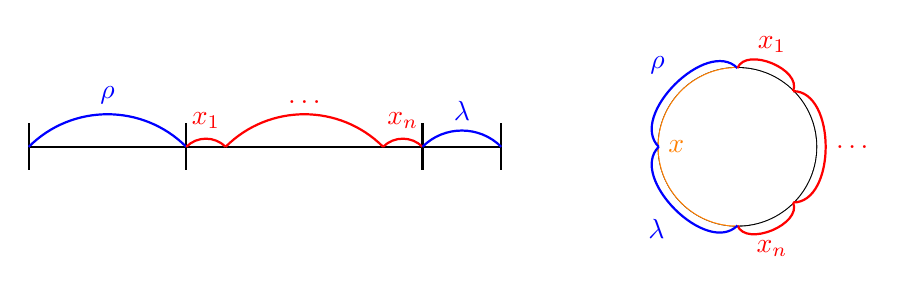
\begin{tikzpicture}
    \def \r {1}
    \coordinate (A) at (-9,0);
    \coordinate (B) at (-7,0);
    \coordinate (C) at (-4,0);
    \coordinate (D) at (-3,0);

    \draw[thick] (A) -- (D);
    \draw[thick] (A) -- ++(0,-0.3);
    \draw[thick] (A) -- ++(0,0.3);
    \draw[thick] (B) -- ++(0,-0.3);
    \draw[thick] (B) -- ++(0,0.3);
    \draw[thick] (C) -- ++(0,-0.3);
    \draw[thick] (C) -- ++(0,0.3);
    \draw[thick] (D) -- ++(0,-0.3);
    \draw[thick] (D) -- ++(0,0.3);

    \draw[thick,blue, bend left = 45] (A) to node[midway, above, blue]{\(\rho\)} (B);
    \draw[thick,red, bend left = 45] (B) to node[midway, above, red]{\(x_1\)} (-6.5,0);
    \draw[thick,red, bend left = 45] (-6.5,0) to node[midway, above, red]{\(\ldots\)} (-4.5,0);
    \draw[thick,red, bend left = 45] (-4.5,0) to node[midway, above, red]{\(x_n\)} (C);
    \draw[thick,blue, bend left = 45] (C) to node[midway, above, blue]{\(\lambda\)} (D);
    

    \draw[thick] (0,0) circle (\r);
    \draw[thick,orange] (0,-\r) arc[start angle=270, end angle=90, radius=\r] -- cycle;
    \fill[white] (0,0) circle (\r);
    \node[anchor=west, orange] at (-\r,0) {\(x\)};
    \draw[thick,blue, bend left = 90] (-\r,0) to node[midway, above left, blue]{\(\rho\)} (0,\r);
    \draw[thick,red, bend left = 90] (0,\r) to node[midway, above, red]{\(x_1\)} ({cos(45)},{sin(45)});
    \draw[thick,red, bend left = 90] ({cos(45)},{sin(45)}) to node[midway, right, red]{\(\ldots\)}({cos(-45)},{sin(-45)});
    \draw[thick,red, bend left = 90] ({cos(-45)},{sin(-45)}) to node[midway, below, red]{\(x_n\)} (0,-\r);
    \draw[thick,blue, bend left = 90] (0,-\r) to node[midway, below left, blue]{\(\lambda\)} (-\r,0);
    
  \end{tikzpicture}
  \caption{Rappresentazione grafica della definizione di codice circolare}\label{fig:circular_factorization}
\end{figure}

\begin{example}{}
  Il codice \(X = \set{ab,ba,bb}\) non è circolare. Considerando infatti la parola \(abab\). Si ha che, fissando \(\rho = a, \lambda = b\) che \(\lambda\rho = ba \in X\) e che \(\rho ba \lambda = abab \in \set{\rho}X^*\set{\lambda}\).
  Passando alla fattorizzazione circolare, è possibile ottenre \(abab\) nei seguenti modi:
  \begin{figure}[H]
    \centering
    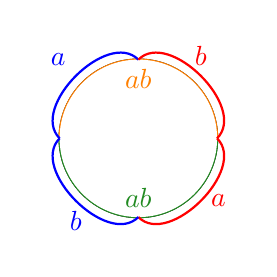
\begin{tikzpicture}
      \def \r {1}
      \draw[thick] (0,0) circle (\r);
      \draw[thick,orange] (-\r,0) arc[start angle=180, end angle=0, radius=\r] -- cycle;
      \draw[thick,ForestGreen] (-\r,0) arc[start angle=180, end angle=360, radius=\r] -- cycle;
      \fill[white] (0,0) circle (\r);
      \node[anchor=north, orange] at (0,\r) {\(ab\)};
      \node[anchor=south, ForestGreen] at (0,-\r) {\(ab\)};
      \draw[thick,blue, bend left = 90] (-\r,0) to node[midway, above left, blue]{\(a\)} (0,\r);
      \draw[thick,red, bend left = 90] (0,\r) to node[midway, above, red]{\(b\)} (\r,0);
      \draw[thick,red, bend left = 90] (\r,0) to node[midway, right, red]{\(a\)}(0,-\r);
      \draw[thick,blue, bend left = 90] (0,-\r) to node[midway, below, blue]{\(b\)} (-\r,0);
    
    \end{tikzpicture}
    \hspace{2cm}
    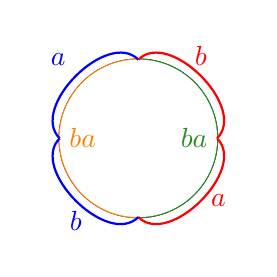
\begin{tikzpicture}
      \def \r {1}
      \draw[thick] (0,0) circle (\r);
      \draw[thick,orange] (0,-\r) arc[start angle=270, end angle=90, radius=\r] -- cycle;
      \draw[thick,ForestGreen] (0,-\r) arc[start angle=-90, end angle=90, radius=\r] -- cycle;
      \fill[white] (0,0) circle (\r);
      \node[anchor=west, orange] at (-\r, 0) {\(ba\)};
      \node[anchor=east, ForestGreen] at (\r,0) {\(ba\)};
      \draw[thick,blue, bend left = 90] (-\r,0) to node[midway, above left, blue]{\(a\)} (0,\r);
      \draw[thick,red, bend left = 90] (0,\r) to node[midway, above, red]{\(b\)} (\r,0);
      \draw[thick,red, bend left = 90] (\r,0) to node[midway, right, red]{\(a\)}(0,-\r);
      \draw[thick,blue, bend left = 90] (0,-\r) to node[midway, below, blue]{\(b\)} (-\r,0);
    
    \end{tikzpicture}
    \caption{Rappresentazione grafica della definizione di codice circolare}
  \end{figure}
  Inoltre, qualsiasi codice che contenga una parola che è potenza di una lettera non può essere circolare.
  Questo si può banalmente vedere considerando il caso in cui \(a^n \in X\) con \(a \in A\). Si ha necessariamente che \(a^{2n} = a^{\frac{n}{2}} a^n a^{\frac{n}{2}} \in X^*\) e dunque la fattorizzazione non è circolarmente univoca.
\end{example}

\begin{proposition}{Chi troppo vuole...}
  Sia \(X\) codice su \(A\) finito, circolare e massimale. Allora \(X = A\).
\end{proposition}

\begin{proof}
  Dal \Cref{cor:schutz_maximality_completeness} e dalla \Cref{prop:finite_complete_codes_contains_powers}, sappiamo che se \(X\) è massimale e finito, \(\forall a \in A, \exists n_a \geq 1 \st a^{n_a} \in X\)
  Poiché \(X\) è circolare, \(\forall a, n_a = 1\).
  Dunque \(A \subseteq X \implies X = A\), essendo \(A\) codice massimale su \(A^*\)
\end{proof}

\begin{theorem}{Restivo}
  Sia \(X\) codice su \(A\). Allora
  \begin{enumerate}
    \item \(X\) codice a ritardo di sincronizzazione finito \(\implies X\) circolare e a \keyword{parassitismo limitato}.
    \item \(X\) codice regolare, circolare e a parassitismo limitato \(\implies X\) codice a ritardo di sincronizzazione finito
  \end{enumerate}
\end{theorem}

\begin{note}{}
  Il parassitismo (limitato) non è stato trattato nel corso, poiché esula dagli argomenti principali.
  In maniera informale, un codice \(X\) ha parassitismo se esistono parole di \(X\) che contengono al loro interno parole di \(X^*\)
  Si parla di parassitismo limitato se esiste un limite superiore \(p\) alla lunghezza delle parole di \(X^*\) che possono essere contenute all'interno di parole di \(X\).
  Più formalmente,
  \[X \text{ ha parassitismo} \iff (A^+X^* A^*\cup A^*X^*A^+) \cap X \neq \emptyset\]
  \[X \text{ ha parassitismo limitato} \iff \exists p > 1 \st A^*X^p A^* \cap X = \emptyset\]

  Ciò che è d'interesse per questo corso, è che qualsiasi codice finito ha necessariamente parassitismo limitato.
\end{note}

\begin{corollary}{}
  Sia \(X\) codice finito, allora \(X\) codice a ritardo di sincronizzazione finito \(\iff X\) circolare.
\end{corollary}

\begin{corollary}{}
  Un codice a ritardo di sincronizzazione finito, binario e adattato a una sorgente propria \textbf{non} è ottimale (a meno che \(\# \SCal = 2\)).
\end{corollary}

\begin{proof}
  Dal corollario precedente, un codice a ritardo di sincronizzazione finito e adattato a una sorgente propria è circolare.
  Sappiamo inoltre che un codice binario ottimale è anche massimale.
  Dunque, per la proposizione precedente, l'unico codice finito binario circolare ottimale è l'alfabeto stesso, che però non è adattato a una sorgente propria con più di due simboli.
\end{proof}

\begin{definition}{Insiemi resto modificati}
  Sia \(X\) codice su \(A\). Definiamo l'insieme dei \keyword{resti modificati} di \(X\) come
  \begin{equation*}
    R_n'(X) = \begin{cases}
    Suff(X)\setminus (X \cup \set{\varepsilon}) & n = 1\\
    {R_{n-1}'(X)}^{-1}X \cup X^{-1}R_{n-1}'(X) & n > 1
    \end{cases}
  \end{equation*}
\end{definition}

\begin{theorem}{Levenshtein}
  \(X\) circolare \(\iff \exists n \geq 1 \st R_n'(X) = \emptyset\)
\end{theorem}

\begin{observation}{}
  Per \(X\) codice (finito),
  \[R_1 = X^{-1}X\setminus \set{\varepsilon} \subseteq Suff(X) \setminus (X \cup \set{\varepsilon}) = R_1' \implies \forall n \geq 1, R_n \subseteq R_n'\]
  Questo è un altro modo per dimostrare che se \(X\) ha ritardo di sincronizzazione finito, allora ha ritardo di decifrazione finito.
  Infatti se ha ritardo di sincronizzazione finito, allora ha \(R_n' = \emptyset\) per qualche \(n\), dunque anche \(R_n = \emptyset\) per lo stesso \(n\), e quindi ha ritardo di decifrazione finito per teoremi visti prima 
\end{observation}

\begin{example}{}
  \(X = \set{a,ba,bb}\) \textbf{non} è circolare.
  Infatti \(R_1' = Suff(X) \setminus (X \cup \set{\varepsilon}) = \set{b}\).
  Inoltre \(R_2' = {R_1'}^{-1}X \cup X^{-1}R_1' = \set{a,b}\).
  \(R_3' = \set{\varepsilon, a ,b}\),\(R_4' = \set{\varepsilon, a ,b, ba,bb} = R_n' \forall n \geq 4\).

  Invece \(X' = \set{ab,aab}\) circolare: \(R_1' = \set{b}, R'_2 = \emptyset\)
  Anche \(X'' = \set{ab,aba,ba^3,b^2a}\) è circolare:
  \(R_1' = \set{a,b,a^2,ba,a^3}, R_2' = \set{b,ba,a^3,a^2}, R_3' = \set{a^3,ba,a^3}, R_4' = \set{a^3}, R_5' = \emptyset\)
\end{example}


\chapter{Entropia multivariabile e processi stocastici}

Nel precedente capitolo, abbiamo introdotto il concetto di entropia di una sorgente, vedendo che essa è il limite inferiore del costo di codifica. 
In questo capitolo, approfondiremo il concetto di entropia, analizzandolo più formalmente, introducendo alcune sue proprietà e generalizzandolo a più variabili aleatorie.

\section{Rimandi di teoria della probabilità ed Entropia}

Prima di procedere, facciamo un breve richiamo ad alcuni concetti di teoria della probabilità necessari per la comprensione dei concetti che andremo a trattare in questo capitolo.
Uno \keyword{spazio di probabilità} è una tripla \((\Omega, \mathcal{F}, \Prob)\) dove
\begin{itemize}
  \item \(\Omega\) è un insieme non vuoto, detto spazio dei campioni (o spazio campione);
  \item \(\mathcal{F} \subseteq \mathcal{P}(\Omega)\) è una \(\sigma\)-algebra su \(\Omega\), cioè un insieme di sottoinsiemi di \(\Omega\), incluso lo stesso \(\Omega\), chiuso rispetto all'unione, al complemento e alle unioni numerabili\footnote{$\mathcal{F}$ è: chiuso rispetto all'unione se $\forall A,B \in \mathcal{F}: (A \cup B) \in \mathcal{F}$; chiuso rispetto al complemento se $\forall A \in \mathcal{F}: \bar{A}=(\mathcal{F} \setminus A) \in \mathcal{F}$; chiuso rispetto alle unioni numerabile se $\mathcal{F}$ è infinito numerabile e $\forall \set{A_i}_{i \in \mathbb{N}}: \bigcup_{A \in \set{A_i}}A \in \mathcal{F}$.};
  \item \(\Prob: \mathcal{F} \to [0,1]\) è una misura di probabilità, cioè una funzione tale che \(\Prob[\Omega] = 1, \Prob[\emptyset] = 0\) e che è \(\sigma\)-additiva, ovvero per ogni famiglia numerabile di eventi disgiunti \({\{A_i\}}_{i \in \mathbb{N}} \subseteq \mathcal{F}\) si ha che
  \[\Prob\left[\bigcup_{i=1}^{\infty} A_i\right] = \sum_{i=1}^{\infty} \Prob[A_i]\]
\end{itemize}

Una \keyword{variabile aleatoria discreta} su uno spazio di probabilità \((\Omega, \mathcal{F}, \Prob)\) è un applicazione misurabile \(S: \Omega \to \SCal\), dove \(\SCal\) è un insieme discreto (finito o numerabile), che ad un evento in $\Omega$ associa un simbolo in $\SCal$.

Essendo \(S\) misurabile, è possibile associare una funzione \q{massa} di probabilità (distribuzione su \(\SCal\)) \(p: \SCal \to [0,1]\) definita come \(p(s) = \Prob[S=s] = \Prob[S^{-1}(s)]\)\footnote{La notazione $\Prob[X=x]$ risulta spesso comoda, ma è abusiva: la notazione formalmente corretta è $\Prob[S^{-1}(s)]$ poiché $\Prob$ è definita su $\mathcal{F}$ e $S^{-1}(s) \in \mathcal{F}$.}.
Per chiarezza e semplicità, assumeremo che la variabile $A$ abbia alfabeto $\mathcal{A}$, che $B$ abbia alfabeto $\mathcal{B}$ e così via.

\begin{definition}{Entropia di una variabile aleatoria}
  Sia \(X\) variabile aleatoria discreta con distribuzione di probabilità \(p\).
  L'\keyword{entropia} di \(X\) è definita come
  \[H(X) = -\sum_{x \in \mathcal{X}} p(x) \log( p(x))= \EV{\log(\frac{1}{p(x)})}\]
\end{definition}

A seguito del teorema di Shannon (\Cref{thm:shannon}), possiamo interpretare questa quantità come il limite inferiore del costo di codifica per una sorgente binaria.
Dunque possiamo vedere l'entropia come la più corta descrizione binaria del valore di \(X\), o in altre parole il numero medio di domande binarie necessarie per identificare il valore di \(X\). Insomma, $H(X)$ rappresenta il grado di incertezza sul valore emesso da $X$.

\begin{definition}{Definizione assiomatica dell'entropia di Shannon}
  Sia \({(H_m)}_{m \geq 1}\) una famiglia di funzioni, di cui ogni \(H_m \in {(H_m)}_{m \geq 1}\) è una funzione a \(m\) variabili con le seguenti proprietà:
  \begin{description}
    \item[simmetria]: \(\forall \sigma \in S_m: H_m(p_1,\ldots,p_m) = H_m(p_{\sigma(1)},\ldots,p_{\sigma(m)})\), con \( S_m\) insieme delle permutazioni di \(\set{1,\ldots,m}\). In altre parole, l'entropia non dipende dall'ordine in cui i simboli appaiono nell'alfabeto, ma solo dalla distribuzione $p$.
    \item[normalizzazione]: \(H_2\left(\frac{1}{2}, \frac{1}{2}\right) = 1\).
    \item[continuità]: \(H_2(p,1-p)\) funzione continua di \(p\).
    \item[raggruppamento]:
    \[H_m(p_1,p_2,p_3,\ldots,p_m) = H_{m-1}(p_1 + p_2,p_3,\ldots,p_m)+(p_1+p_2)H_2\left(\frac{p_1}{p_1+p_2},\frac{p_2}{p_1+p_2}\right)\]
  \end{description}
\end{definition}

Presa questa definizione, si vede che l'unica implementazione possibile per l'entropia è \[H_m(p_1,\ldots,p_m) = - \sum_{i=1}^{m} p_i \log(p_i)\] preso un qualsiasi \(m\geq 1\).

A questo punto, introduciamo il concetto di variabile aleatoria multipla ed estendiamo l'entropia a tale caso.

\begin{definition}{Entropia Congiunta}
  Siano \(X, Y\) variabili aleatorie. Definiamo la \keyword{variabile aleatoria congiunta}, rappresentata dalla coppia \((X,Y)\), come:
  \[(X,Y): \omega \in \Omega \mapsto (X(\omega), Y(\omega)) \in \mathcal{X} \times \mathcal{Y}\]
  
  La cui funzione di massa di probabilità congiunta è data da
  \[p(x,y) = \Prob[X=x, Y=y] = \Prob[X=x \land Y=y] = \Prob[X^{-1}(x) \cap Y^{-1}(y)]\]
  L'\keyword{entropia congiunta} di \(X\) e \(Y\) è definita come
  \[H(X,Y) = - \sum_{\substack{x \in \mathcal{X},\\ y \in \mathcal{Y}}} p(x,y) \log(p(x,y)) = \EV{\log\left(\frac{1}{p(x,y)}\right)}\]
\end{definition}

\begin{definition}{Condizionamento}
  Dati \(A,B \subseteq \Omega\), definiamo \(A|B\) l'evento \(A\) condizionato da \(B\) (\qi{A dato B}) come l'evento tale che
  \[\Prob[A|B] = \frac{\Prob[A \cap B]}{\Prob[B]}\]

  In particolare, se \(X,Y\) sono variabili aleatorie, definiamo \(p(y|x) = \Prob[Y=y|X=x]\)

  Si ha dunque che \(\forall x \in \mathcal{X}, y \in \mathcal{Y}, p(y|x) = \frac{p(x,y)}{p(x)}\), cioè \(p(x,y) = p(x)p(y|x)\).
\end{definition}

Possiamo notare che  \(\forall x \in \mathcal{X}\) fissato, \(p(y|x)\) è una distribuzione di probabilità su \(\mathcal{Y}\).
Infatti,\footnote{Date \(X,Y\) variabili aleatorie, si ha che \(\sum_{y \in \mathcal{Y}} p(x,y) = p(x), \forall x \in \mathcal{X}\) per la proprietà di marginalizzazione di una funzioni di massa di probabilità congiunta.
In altre parole, data una funzione di massa di probabilità congiunta \(p(x,y)\), è sempre possibile ricavare le distribuzioni marginali $p(x)$ e $p(y)$. L'operazione inversa è possibile solo quando $X$ e $Y$ sono indipendenti, ovvero quando si osserva $p(x,y)=p(x)p(y)$.}
\[\sum_{y \in \mathcal{Y}} p(y|x) = \sum_{y \in \mathcal{Y}} \frac{p(x,y)}{p(x)} = \frac{1}{p(x)} \sum_{y \in \mathcal{Y}} p(x,y) = \frac{p(x)}{p(x)} = 1\]

Possiamo vedere $p(y|x)$ come funzione massa di probabilità di una variabile aleatoria \(Y|X=x\).

\begin{definition}{Entropia Condizionata}
  Siano \(X,Y\) variabili aleatorie.
  L'\keyword{entropia condizionata} di \(Y|X\) è definita come
  \[H(Y|X) = \sum_{x \in \mathcal{X}} p(x) H(Y|X=x) = - \sum_{x \in \mathcal{X}} p(x) \sum_{y \in \mathcal{Y}} p(y|x) \log(p(y|x)) = \]
  \[= -\sum_{\substack{x \in \mathcal{X}\\y \in \mathcal{Y}}} p(x,y) \log (p(y|x)) = \EV{\log\left(\frac{1}{p(y|x)}\right)}[x,y]\]
  
  ovvero la media delle entropie di \(Y|X=x\) al variare di \(x\), pesata secondo la probabilità \(p(x)\).
\end{definition}

Definite queste quantità, vediamo come si relazionano tra di loro, partendo dalla prima regola di catena.

\begin{proposition}{Regola di catena}
  Date \(X,Y\) variabili aleatorie, si ha che
  \[H(X,Y) = H(X) + H(Y|X)\]
\end{proposition}

\begin{proof}
  \[H(X,Y) =-\sum_{\substack{x \in \mathcal{X},\\ y \in \mathcal{Y}}} p(x,y) \log(p(x,y)) = -\sum_{\substack{x \in \mathcal{X},\\ y \in \mathcal{Y}}} p(x,y) \log(p(x)p(y|x)) = \]
  \[= - \sum_{\substack{x \in \mathcal{X},\\ y \in \mathcal{Y}}} p(x,y)\left(\log(p(x)) + \log(p(y|x))\right)  = - \sum_{\substack{x \in \mathcal{X},\\ y \in \mathcal{Y}}} p(x,y) \log(p(x)) - \sum_{\substack{x \in \mathcal{X},\\ y \in \mathcal{Y}}} p(x,y) \log(p(y|x)) =\]
  \[=- \sum_{x \in \mathcal{X}} \log(p(x))\sum_{y \in \mathcal{Y}} p(x,y)  - \sum_{\substack{x \in \mathcal{X},\\ y \in \mathcal{Y}}} p(x,y) \log(p(y|x)) = H(X) + H(Y|X)\]
\end{proof}

\begin{example}{}
  Prendiamo in considerazione due variabili aleatorie quaternarie \(X,Y\) la cui probabilità congiunta è data dalla seguente tabella:
  \begin{center}
    \begin{tabular}{c|c c c c}
      \(Y \backslash X\) & \(a\) & \(b\) & \(c\) & \(d\) \\
      \hline
      \(1\) & \(\frac{1}{8}\) & \(\frac{1}{16}\) & \(\frac{1}{32}\) & \(\frac{1}{32}\) \\
      \(2\) & \(\frac{1}{16}\) & \(\frac{1}{8}\) & \(\frac{1}{32}\) & \(\frac{1}{32}\) \\
      \(3\) & \(\frac{1}{16}\) & \(\frac{1}{16}\) & \(\frac{1}{16}\) & \(\frac{1}{16}\) \\
      \(4\) & \(\frac{1}{4}\) & \(0\) & \(0\) & \(0\) \\
    \end{tabular}
  \end{center}

  Verifichiamo che \(H(X) = \frac{7}{4}\).
  Per calcolare l'entropia di \(X\), dobbiamo prima calcolare la distribuzione di probabilità marginale di \(X\):
  \begin{itemize}
    \item \(p(a) = \frac{1}{8} + \frac{1}{16} + \frac{1}{16} + \frac{1}{4} = \frac{1}{2}\)
    \item \(p(b) = \frac{1}{16} + \frac{1}{8} + \frac{1}{16} + 0 = \frac{1}{4}\)
    \item \(p(c) = \frac{1}{32} + \frac{1}{32} + \frac{1}{16} + 0 = \frac{1}{8}\)
    \item \(p(d) = \frac{1}{32} + \frac{1}{32} + \frac{1}{16} + 0 = \frac{1}{8}\)
  \end{itemize}
  Abbiamo dunque che
  \[H(X) = \frac{1}{2}\log(2)+\frac{1}{4}\log(4)+\frac{1}{8}\log(8)+\frac{1}{8}\log(8) = \]
  \[= \frac{1}{2}+\frac{1}{4}\cdot 2 + \frac{2}{8} \cdot 3 = \frac{7}{4}\]
  
  Verifichiamo ora che \(H(Y) = 2\).
  Analogamente a prima, calcoliamo la distribuzione di probabilità marginale di \(Y\):
  \begin{itemize}
    \item \(p(1) = \frac{1}{8} + \frac{1}{16} + \frac{1}{32} + \frac{1}{32} = \frac{1}{4}\)
    \item \(p(2) = \frac{1}{16} + \frac{1}{8} + \frac{1}{32} + \frac{1}{32} = \frac{1}{4}\)
    \item \(p(3) = \frac{1}{16} + \frac{1}{16} + \frac{1}{16} + \frac{1}{16} = \frac{1}{4}\)
    \item \(p(4) = \frac{1}{4} + 0 + 0 + 0 = \frac{1}{4}\)
  \end{itemize}
  Dunque
  \[H(Y) = 4 \cdot \frac{1}{4} \log(4) = 2\]

  Verifichiamo ora che \(H(X,Y) = \frac{27}{8}\).
  In questo caso è sufficiente calcolare direttamente l'entropia congiunta:
  \[H(X,Y) = 2\cdot\frac{1}{8}\cdot 3 + 6\cdot\frac{1}{16}\cdot 4 + \frac{1}{4}\cdot 2 + 4 \cdot \frac{1}{32}\cdot 5= \]
  \[= \frac{6}{8} + \frac{24}{16} + \frac{2}{4} + \frac{20}{32} = \frac{27}{8}\]
  

  Infine, si ha che \(H(X|Y) = H(X,Y)-H(X) = \frac{27}{8} - \frac{7}{4} = \frac{13}{8}\) e che \(H(Y|X) = H(X,Y)-H(Y) = \frac{27}{8} - 2 = \frac{11}{8}\).
\end{example}

Dall'esempio precedente, possiamo osservare che l'entropia congiunta è simmetrica rispetto alle variabili coinvolte, mentre l'entropia condizionata no.
In generale, \(H(X|Y) \neq H(Y|X)\) e \(H(X,Y) = H(Y,X)\).

Tuttavia, la regola di catena ci assicura che
\[H(Y)+H(X|Y)=H(Y,X)=H(X,Y) = H(X)+H(Y|X)\]
ovvero
\[H(Y) - H(Y|X) = H(X) - H(X|Y)\]

Possiamo generalizzare questo risultato a più variabili aleatorie.

\begin{proposition}{Regola di catena con condizionamento}
  Date \(X,Y,Z\) variabili aleatorie, si ha che
  \[H(X,Y|Z) = H(X|Z) + H(Y|X,Z)\]
  ossia
  \[- \sum_{\substack{x \in \mathcal{X},\\y\in\mathcal{Y},\\z \in \mathcal{Z}}} p(x,y,z) \log(p(x,y|z)) = -\sum_{\substack{x\in\mathcal{X},\\z\in\mathcal{Z}}} p(x,z)\log(p(x|z)) - \sum_{\substack{x \in \mathcal{X},\\y \in \mathcal{Y},\\z \in \mathcal{Z}}} p(x,y,z) \log(p(y|x,z))\]
\end{proposition}


\begin{definition}{Divergenza di Kullback-Leibler (entropia relativa)}
  Siano \(p,q\) due distribuzioni di probabilità su uno stesso insieme discreto \(\mathcal{X}\).
  La \keyword{divergenza di Kullback-Leibler} tra \(p\) e \(q\) è definita come
  \[D_{KL}(p ||q) = \sum_{x \in \mathcal{X}} p(x) \log\left(\frac{p(x)}{q(x)}\right) \]
\end{definition}

\begin{note}{}
  Essendo che possono esistere \(x\) tali che \(q(x) = 0\) e \(p(x) > 0\), la divergenza di Kullback-Leibler può essere infinita.
\end{note}

La divergenza di Kullback-Leibler è spesso interpretata come una distanza, anche se non ne rispetta propriamente le proprietà matematiche.

Infatti non sono soddisfatte la simmetria, \(D(p||q) \neq D(q||p)\), e la disuguaglianza triangolare.
La divergenza di Kullback-Leibler è però \textit{definita positiva}, ovvero \(D_{KL}(p||q) \geq 0\) con uguaglianza se e solo se \(p=q\).\footnote{Questo segue in maniera diretta dall'\Cref{eq:gibbs} vista in precedenza}

\begin{definition}{Mutua Informazione}
  Siano \(X,Y\) variabili aleatorie congiunte.
  La \keyword{mutua informazione} tra \(X\) e \(Y\) è definita come
  \[I(X;Y) = D_{KL}(p(x,y) || p(x)p(y)) = \sum_{\substack{x \in \mathcal{X}\\y \in \mathcal{Y}}} p(x,y) \log\left(\frac{p(x,y)}{p(x)p(y)}\right)\]

  Essendo che \(p(x,y)=p(x)p(y), \forall x\in\mathcal{X}, y\in\mathcal{Y} \iff\) \(X\) e \(Y\) sono indipendenti, si ha che \(I(X;Y) = 0 \iff\) \(X\) e \(Y\) sono indipendenti.
\end{definition}

Intuitivamente, la mutua informazione misura la quantità di informazione, come riduzione di incertezza, che una variabile aleatoria fornisce sull'altra.
Questa è ovviamente nulla quando le due variabili sono indipendenti.

Si ha inoltre che
\[I(X;Y) = \sum_{\substack{x \in \mathcal{X}\\y \in \mathcal{Y}}} p(x,y) \log\left(\frac{p(x,y)}{p(x)p(y)}\right) = \]
\[= \sum_{\substack{x \in \mathcal{X}\\y \in \mathcal{Y}}} p(x,y) \log\left(\frac{p(y|x)}{p(y)}\right) = \sum_{\substack{x\in\mathcal{X}\\y\in\mathcal{Y}}}p(x,y)\log(p(y|x)) - \sum_{y\in\mathcal{Y}}\log(p(y))\sum_{x\in\mathcal{X}}p(x,y)\]
\[= H(Y)-H(Y|X)\]


Un modo intuitivo per visualizzare le relazioni tra le varie quantità di informazione viste finora è tramite i diagrammi di Venn modificati come in \Cref{fig:venn_info}.

\begin{figure}[H]
  \centering
  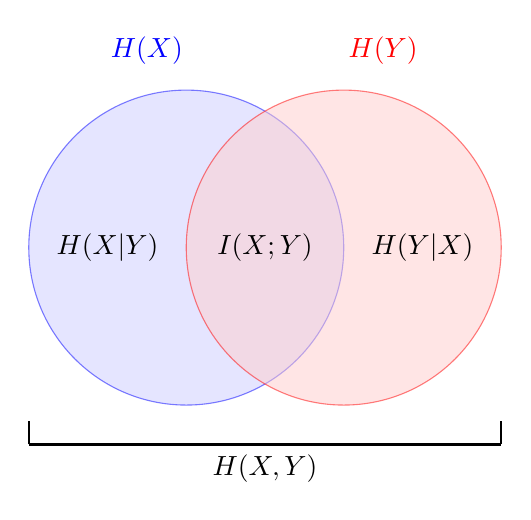
\begin{tikzpicture}
    \def \r {2} % radius of circles
    \def \d {2} % distance between centers

    % Draw circles
    \draw[fill=blue!20, draw=blue, opacity=0.5] (-\d/2,0) circle (\r);
    \draw[fill=red!20, draw=red, opacity=0.5] (\d/2,0) circle (\r);

    % Labels
    \node at (-\d/2-0.5, \r + 0.5) [blue] {\(H(X)\)};
    \node at (\d/2+0.5, \r + 0.5) [red] {\(H(Y)\)};
    \node at (0,0) {\(I(X;Y)\)};
    \node at (-\d, 0) {\(H(X|Y)\)};
    \node at (\d, 0) {\(H(Y|X)\)};

    \draw[thick] (-\d/2-\r,-\r-0.5) to node[midway, below, ] {\(H(X,Y)\)} (\d/2+\r,-\r-0.5);
    \draw[thick] (-\d/2-\r,-\r-0.5) -- ++(0,0.3);
    \draw[thick] (\d/2+\r,-\r-0.5) -- ++(0,0.3);
  \end{tikzpicture}
  \caption{Diagramma di Venn per le quantità di informazione.}\label{fig:venn_info}
\end{figure}

\begin{definition}{Informazione mutua condizionata}
  Date \(X,Y,Z\) variabili aleatorie, la \keyword{mutua informazione condizionata} tra \(X\) e \(Y\) dato \(Z\) è definita come
  \[I(X;Y|Z) = H(X|Z) - H(X|Y,Z)\]
\end{definition}

Possiamo dunque generalizzare le regole di catena a \(n\) variabili.

\begin{proposition}{}
  Siano \(X_1, X_2, \ldots, X_n, Y\) variabili aleatorie.
  Si ha che
  \[H(X_1, X_2, \ldots, X_n) = H(X_1) + H(X_2|X_1) + \cdots + H(X_n | X_1, X_2, \ldots, X_{n-1}) = \]
  \[=H(X_1) + \sum_{i=2}^{n} H(X_i | X_{i-1}, \ldots, X_1)\]
  E che
  \[I(X_1, \ldots, X_n; Y) = I(X_1; Y) + I(X_2; Y | X_1) + \cdots + I(X_n; Y | X_1, \ldots, X_{n-1}) = \]
  \[=I(X_1;Y) + \sum_{i=2}^{n} I(X_i; Y | X_{i-1}, \ldots, X_1)\]
\end{proposition}

\subsection{Limiti dell'informazione mutua}\label{subs:mutual_information_limits}

Essendo \(I\) definita in termini di divergenza di Kullback-Leibler, \(I\) è definita positiva, dunque \(I(X;Y) \geq 0\) e l'uguaglianza si verifica se e solo se \(X\) e \(Y\) sono indipendenti.
In tal caso infatti, le due variabili non forniscono alcuna informazione l'una sull'altra.

Da un punto di vista formale, questo si ha perché \(p(x,y)=p(x)p(y)\) per ogni \(x \in \mathcal{X}\) e \(y \in \mathcal{Y}\) se e solo se \(X\) e \(Y\) sono indipendenti.

Poiché \(I(X;Y) = H(X) - H(X|Y)\) e l'entropia è una quantità non negativa, $I$ è massima quando $H(X|Y)=0$. Ciò si verifica quando l'incertezza sull'emissione di $X$ è nulla dopo aver osservato l'emissione di $Y$, ovvero quando $X$ è deterministicamente ricavato da $Y$, ovvero: \footnote{Ricordiamo che dati due insiemi \(A,B\), con \(B^A\) si intende l'insieme delle funzioni da \(A\) a \(B\), come visto nel primo capitolo.}
\[\exists f \in \mathcal{X}^\mathcal{Y} \st X= f\circ Y\]

In tal caso, si ha che \(I(X;Y) = H(X)\).
In particolare, per \(f = id\) si ha che \(I(X;X) = H(X)\), giustificando il significato intuitivo dato all'entropia nel capitolo precedente come misura dell'autoinformazione di una variabile aleatoria.

Infine, notiamo che
\[I(X;Y)\geq 0 \implies H(X) \geq H(X|Y)\]
cioè che \qi{il condizionamento non aumenta l'entropia}. Infatti, intuitivamente, la conoscenza di $Y$ può togliere incertezza dall'emissione di $X$, ma di certo non può aggiungerla. Per questo motivo, si osserva il seguente risultato.

\begin{proposition}{}
  Date \(X_1, X_2, \ldots, X_n\) variabili aleatorie, si ha che
  \(H(X_1, \ldots, X_n)\leq \sum_{i=1}^n H(X_i)\)
\end{proposition}
\begin{proof}
  Si ha
  \[H(X_1, \ldots, X_n) = H(X_1) + \sum_{i=2}^{n}H(X_i|X_{i-1}, \ldots, X_1)\leq \sum_{i=1}^n H(X_i)\]
  poiché \(H(X_i|X_{i-1}, \ldots, X_1) \leq H(X_i)\) per ogni \(i=2,\ldots,n\).
\end{proof}

\section{Catene di Markov e Processi Stocastici}

\begin{definition}{Catena di Markov (3 variabili)}
  Date tre variabili aleatorie \(X, Y, Z\) si dice che formano una \keyword{catena di Markov} in quest'ordine, denotato come \(X \to Y \to Z\) se vale che
  \[\forall x \in X, y \in Y, z \in Z, p(x,y,z) = p(x)p(y|x)p(z|y)\]
\end{definition}

\begin{observation}{}
  Ciò che cambia rispetto alla definizione generale di variabili aleatorie è che \(p(z|x,y) = p(z|y)\), ovvero che \(Z\) è condizionatamente indipendente da \(X\) dato \(Y\),
  ovvero \(p(x,z|y) = p(x|y)p(z|y)\). 
  
  Si ha infatti che in generale 
  \[p(x,z|y) = \frac{p(x,y,z)}{p(y)} = \frac{p(x,y)p(z|x,y)}{p(y)} = p(x|y)p(z|x,y) \]
  e dunque si ha che \(p(z|x,y) = p(z|y)\) se e solo se \(X\) e \(Z\) sono condizionatamente indipendenti dato \(Y\).
\end{observation}

\begin{proposition}[label=prop:markov_chain_third_funcion_second]{}
  Siano \(Y,Z\) variabili aleatorie tali che \(Z = f \circ Y\) per qualche funzione \(f \in \mathcal{Z}^{\mathcal{Y}}\), allora \( \forall X\) variabile aleatoria, \(X \to Y \to Z\).
\end{proposition}
\begin{proof}
  Si ha per ipotesi che
  \begin{equation*}
    p(z|y) = \begin{cases}
      1 & \text{se } z = f(y) \\
      0 & \text{altrimenti}
    \end{cases}
  \end{equation*}
  Allora se \(z\neq f(y)\), \(0= p(z|y)=\sum_{x\in\mathcal{X}}p(x,z|y)\).
  
  Essendo che \(p(x,z|y)\geq 0\), \(\forall x \in \mathcal{X}\), si ha che \(\sum_{x\in\mathcal{X}}p(x,z|y) \iff p(x,z|y)=0 \; \forall x\), e dunque \(0=p(x,z|y) = p(x|y)p(z|y) = p(x|y)\cdot 0\).

  Se invece \(z = f(y)\), allora \(\sum_{z' \in \mathcal{Z}}p(x,z'|y)=p(x,z|y)\) poiché, per \(z'\neq z\), \( p(x,z'|y)=p(z|y)p(x|z,y)=0 \cdot p(x|z,y)\). 
  Ma stando sommando su tutti gli elementi di \(\mathcal{Z}\), si ha che 
  \[\sum_{z' \in \mathcal{Z}}p(x,z'|y) = p(x|y)=p(x|y)\cdot 1 = p(x|y)p(z|y)\]
  Dunque
  \[p(x,z|y) = \sum_{z' \in \mathcal{Z}}p(x,z'|y)= p(x|y)p(z|y)\]
\end{proof}

\begin{proposition}[label=prop:dpi]{Disuguaglianza di Data Processing (DPI)}
  Date \(X,Y,Z\) variabili aleatorie.
  Se \(X \to Y \to Z\) allora \(I(X;Y) \geq I(X;Z)\).

  Inoltre, vale l'uguaglianza se e solo se \(X \to Z \to Y\).
\end{proposition}

\begin{observation}{}
  Questa disuguaglianza ci dice che (nel caso particolare di \(Z = f \circ Y\)), non si può \qi{elaborare} il dato \(Y\) per ottenere più informazioni su \(X\) rispetto a quelle che già si avevano in \(Y\).
\end{observation}

\begin{proof}
  Per la regola di catena,
  \[I(X;Y)+I(X;Z|Y)=I(X;Y,Z) = I(X;Z) + I(X;Y|Z)\]
  Se \(X \to Y \to Z\), abbiamo che \(X\) e \(Z\) sono condizionatamente indipendenti dato \(Y\), dunque \(I(X;Z|Y)=0\) dalla \Cref{subs:mutual_information_limits}
  Allora
  \[I(X;Y) = I(X;Z) + I(X;Y|Z) \]
  Essendo che \(I(X;Y|Z) \geq 0\), si ha la tesi.

  Inoltre, vale l'uguaglianza se e solo se \(I(X;Y|Z)=0\), ovvero se e solo se \(X\) e \(Y\) sono condizionatamente indipendenti dato \(Z\), ovvero \(X\to Z \to Y\).
\end{proof}

È importante notare che l'equazione ricavata nella dimostrazione precedente porta anche a
\[I(X;Y) \geq I(X;Y|Z)\]
Intuitivamente, questa disuguaglianza esprime il concetto che l'informazione che \(Y\) fornisce su \(X\) non può essere aumentata conoscendo \(Z\), se \(X \to Y \to Z\), ovvero se \(X\) e \(Z\) sono condizionatamente indipendenti dato \(Y\).
In altre parole, com'è intuitivo, date due variabili aleatorie \(X\) e \(Z\) tali che data una terza variabile aleatoria \(Y\) queste sono condizionatamente indipendenti, se conosco \(Y\) tutta l'informazione che \(Z\) può fornirmi su \(X\) è già contenuta in \(Y\).

In generale, però, se non vale che \(X \to Y \to Z\), tale disuguaglianza può non essere vera.
Ad esempio, siano \(X, Y\) i.i.d\footnote{Indipendenti e Identicamente Distribuite}, uniformi su \(\{0,1\}\), e sia \(Z = X + Y, \mathcal{Z} = \set{0,1,2}\).
Allora \(I(X;Y) = 0\) poiché sono indipendenti, ma 
\[I(X;Y|Z) = H(X|Z) - H(X|Y,Z) = H(X|Z) - 0 = H(X|Z) = \frac{1}{2}\]

\begin{definition}{Processi stocastici}
  Un \keyword{processo stocastico} \(\underline{X} = {(X_n)}_{n\geq 1}\) è una successione di variabili aleatorie su \(\mathcal{X}\).

  Un processo \(\underline{X}\) è \keyword{stazionario} se \(\forall n, k \geq 1, (x_1, \ldots, x_n) \in \mathcal{X}^n\) si ha che
  \[\Prob[X_1 = x_1, \ldots ,X_n = x_n] = \Prob[X_{k+1} = x_1, \ldots, X_{k+n} = x_n]\]

  In particolare per \(n=1\) si ha che le variabili aleatorie \(X_i\) sono identicamente distribuite.

  Caso particolare, se le variabili aleatorie sono anche indipendenti, si ha un processo \keyword{i.i.d.}
\end{definition}

\begin{note}{}
  % TODO: per l'interpretazione come sorgente è necessaria la stazionarietà? Non necessaria, ma comoda e frequente
  Possiamo interpretare i processi stocastici stazionari come modelli per sorgenti di informazione che generano simboli in modo casuale secondo una certa distribuzione di probabilità nel tempo.

  Si ha che un processo stazionario indipendente corrisponde a una sorgente a memoria zero.
  Essendo questo però un caso particolare, questo modello ci permette di descrivere anche sorgente con memoria, ovvero in cui la probabilità di generare un certo simbolo dipende dai simboli generati in precedenza.
\end{note}

\begin{definition}{Catene di Markov (processi)}
  Un processo stocastico \(\underline{X} = {(X_n)}_{n\geq 1}\) è una \keyword{catena di Markov} se si ha che, 
  \[\begin{aligned}
    \forall n \geq 1, & \forall (x_1, \ldots, x_{n+1}) \in \mathcal{X}^{n+1}, \\
                      & \Prob[X_{n+1} = x_{n+1}|X_n = x_n, \ldots, X_1 = x_1] = \Prob[X_{n+1} = x_{n+1}|X_n = x_n]
  \end{aligned}\]

  Ovvero la probabilità di osservare un certo stato \(X_{n+1}\) dipende solo dallo stato precedente \(X_n\), e non da tutti gli stati precedenti.
\end{definition}

\begin{note}{}
  L'analogia con le sorgenti a memoria zero per i processi stazionari indipendenti potrebbe portare a pensare che le catene di Markov rappresentino solo sorgenti con memoria \(1\), ma in realtà, aggregando più variabili aleatorie insieme è possibile modellare sorgenti con memoria maggiore.
\end{note}

\begin{definition}{Catene tempo invarianti}
    Una catena di Markov si dice \keyword{invariante nel tempo} se \(\forall n \geq 1, \forall x,x'\in\mathcal{X}\)
  \[\Prob[X_{n+1} = x | X_n = x'] = \Prob[X_2 = x | X_1 = x']\]
  
  Ovvero che la probabilità di osservare un certo stato noto il precedente non dipende da in che punto del processo ci si trova.
\end{definition}

Si nota facilmente che una catena di Markov tempo invariante è completamente caratterizzata dalla distribuzione iniziale \(\Prob[X_1 = x]\) e da una matrice \(P\), detta \keyword{matrice di transizione}, tale che \(P_{i,j} = (\Prob[X_2 = j | X_1 = i])\).\footnote{Tecnicamente per poter descrivere la transizione come una matrice è necessario che \(\mathcal{X} = \set{1, \ldots, \abs{\mathcal{X}}}\). Anche se questo non è sempre vero, si può sempre costruire una corrispondenza biunivoca tra gli elementi di \(\mathcal{X}\) e un insieme di interi consecutivi.}

Infatti \(\forall n\geq 1\), 
\[p(x_{n+1}) = \Prob[X_{n+1}=x_{n+1}] = \sum_{x_n\in\mathcal{X}}\Prob[X_n = x_n]P_{x_n,x_{n+1}} = \sum_{x_n\in\mathcal{X}}p(x_n)P_{x_n,x_{n+1}}\]

Vedendo quindi le distribuzioni come vettori riga, si ha che la distribuzione al tempo \(n+1\), denotata come \(p_{n+1}\), si ottiene moltiplicando la distribuzione al tempo \(n\), \(p_n\), per la matrice di transizione \(P\), ovvero
\[p_{n+1} = p_n P\]

\begin{definition}{Distribuzione stazionaria}
Rispetto a una matrice di transizione \(P\), una distribuzione di probabilità \(\mu\) su \(\mathcal{X}\) si dice \keyword{stazionaria} se \(\mu P = \mu\).

Ovvero \(\mu\) è un autovettore sinistro di \(P\) associato all'autovalore \(1\).

Inoltre possiamo dire che se un processo \(\underline{X}\) ha \(P\) come matrice di transizione e distribuzione iniziale \(\mu\) stazionaria, allora \(\underline{X}\) ha \(\mu\) come distribuzione in ogni istante di tempo.
\end{definition}

\begin{proposition}{}
  Se la distribuzione iniziale di una catena \(\underline{X}\) invariante nel tempo è stazionaria, allora \(\underline{X}\) è stazionaria.
\end{proposition}

\begin{definition}{Catene irriducibili e aperiodiche}
  Una catena \(\underline{X}\) si dice \keyword{irriducibile} se
  \[\forall i,h \in \mathcal{X}, \exists n \geq 1 \st \Prob[X_{n+1} = j|X_1 = i] > 0\]

  Una catena \(\underline{X}\) si dice \keyword{aperiodica} se
  \[\forall x \in \mathcal{X}, MCD \set{n\in\N}[\Prob[X_{n+1} = x|X_1=x]>0] = 1\]
\end{definition}

Si dimostra che una catena invariante nel tempo, aperiodica e irriducibile ha un'unica distribuzione stazionaria e che indipendentemente dalla distribuzione iniziale, se \(\mu\) è tale distribuzione stazionaria, si ha che \[\lim_{n\to\infty} p_n = \mu\]

\begin{example}{}
  Sia \(\mathcal{X} = \set{1,2}\). La matrice di transizione \(P\) di una catena \(\underline{X}\) è individuata da \(\alpha = \Prob[X_2 = 2 | X_1 = 1]\) e \(\beta = \Prob[X_2 = 1 | X_1 = 2]\) come
  \begin{equation*}
    P = \begin{pmatrix}
      1-\alpha & \alpha \\
      \beta & 1-\beta
    \end{pmatrix}
  \end{equation*}
  Se \(p_n = (\Prob[X_n = 1], \Prob[X_n = 2])\), allora \(p_{n+1} = p_n P\).

  La distribuzione stazionaria \(\mu = (\mu(1), \mu(2))\) è tale che \(\mu = \mu \cdot P\), e dunque soddisfa il sistema
  \begin{equation*}
    \begin{cases}
      \mu(1) = \mu(1)(1-\alpha) + \mu(2) \beta \\
      \mu(2) = 1 - \mu(1)
    \end{cases}
  \end{equation*}
  Risolvendo si ottiene che \(\mu = \left(\frac{\beta}{\alpha+\beta}, \frac{\alpha}{\alpha+\beta}\right)\)
\end{example}

\begin{definition}{Tasso di entropia di un processo stocastico}
  Sia \(\underline{X} = {(X_n)}_{n\geq 1}\) un processo stocastico.
  Il \keyword{tasso di entropia} (\keyword{entropy rate}) di \(\underline{X}\) è, se esiste,
  \[H(\underline{X}) = \lim_{n\to\infty} \frac{1}{n} H(X_1, X_2, \ldots, X_n)\]
\end{definition}

Il tasso entropico è un tentativo di generalizzare ai processi il concetto di entropia congiunta.
Tale però è solo un tentativo, poiché non è detto che il limite esista.

Se le variabili aleatorie \(X_i\) sono i.i.d., allora dalla regola di catena
  \[H(X_1, X_2, \ldots, X_n) = H(X_1) + \sum_{i=2}^n H(X_i|X_{i-1}, \ldots, X_1) = \sum_{i=1}^n H(X_i) = n H(X_1)\]

Dunque in questo caso \(H(\underline{X}) = H(X_1)\).\footnote{Essendo i.i.d si ha che \(H(X_1) = H(X_i), \forall i\).}

Si può mostrare che però, già togliendo la sola ipotesi di indipendenza, il limite può non esistere.

\begin{theorem}{}
  Se \(\underline{X}\) è stazionario, il tasso di entropia esiste e coincide con
  \[H'(\underline{X}) = \lim_{n\to\infty} H(X_n|X_{n-1}, \ldots, X_1)\]
\end{theorem}

\begin{proof}
  \(\forall n \geq 1\), essendo che il condizionamento non aumenta l'entropia, si ha che
  \[H(X_{n+1}|X_n, \ldots, X_1)\leq H(X_{n+1}|X_n, \ldots, X_2)\]
  Essendo che \(\underline{X}\) è stazionario, si ha che
  \[H(X_{n+1}|X_n, \ldots, X_2) = H(X_n|X_{n-1}, \ldots, X_1)\]
  Dunque la successione \(a_n = H(X_n|X_{n-1}, \ldots, X_1)\) è decrescente di termini non negativi, e dunque converge, ovvero \(H'(\underline{X})\) esiste.

  Inoltre, dalla regola di catena, \(\frac{1}{n} H(X_1, \ldots, X_n) = \frac{1}{n}\left(H(X_1) +\sum_{i=2}^n H(X_i|X_{i-1}, \ldots, X_1)\right)\), cioè \(\frac{1}{n} H(X_1, \ldots, X_n)\) è la media dei primi \(n\) termini della successione \(a_n\).

  Per il teorema della media di Cesàro\footnote{Il teorema della media di Cesàro afferma che se una successione \(a_n\) ammette limite, allora la media aritmetica delle sue medie parziali converge allo stesso limite. In termini più formali, dato \(\sigma_n = \frac{1}{n}\sum_{i=1}^n a_i\), si ha \[\lim_{n\to\infty} \sigma_n = \lim_{n\to\infty} a_n\]}, si ricava \(H(\underline{X}) = H'(\underline{X})\).
\end{proof}

Se \(\underline{X}\) è una catena di Markov stazionaria, si ha che
\[H(\underline{X}) = \lim_{n\to\infty}H(X_n|X_{n-1}, \ldots, X_1) = \lim_{n\to\infty} H(X_n|X_{n-1}) = H(X_2|X_1)\]

Inoltre se \(P\) è la matrice di transizione della catena e \(\mu\) la sua distribuzione stazionaria, si ha che
\[H(\underline{X}) = H(X_2|X_1) = -\sum_{i,j\in \mathcal{X}} \mu(i) P_{ij} \log P_{ij}\]

Essendo il tasso di entropia una quantità definita al limite, tutte le proprietà che abbiamo visto valgono anche per catene di Markov non stazionarie ma la cui distribuzione converge a quella stazionaria, ovvero catene invariate nel tempo, aperiodiche e irriducibili.

\begin{example}{}
  Per la catena di Markov dell'esempio precedente, si ha che
  \[H(\underline{X}) = -\mu(1)((1-\alpha)\log(1-\alpha) + \alpha \log \alpha) - \mu(2)(\beta \log \beta + (1-\beta) \log (1-\beta))\]
  \[=\frac{\beta}{\alpha+\beta} H(\alpha) + \frac{\alpha}{\alpha+\beta} H(\beta)\]

  Dove \(H(p) = -p \log(p) - (1-p) \log (1-p)\) è l'entropia di una variabile aleatoria di Bernoulli con parametro \(p\).
\end{example}



\input{_chapters/5_block_channel_encoding.tex}
\input{_chapters/6_error_correcting_codes.tex}
\input{_chapters/7_encryption.tex}

\whitepage{}
\makebackcover{}

\end{document}